%!TEX TS-program = xelatex
%!TEX encoding = UTF-8 Unicode
\documentclass[a4paper, 12pt, oneside]{book}
\usepackage{slashbox}
\usepackage{cite}
%\usepackage{chapterbib}
%The chapterbib package facilitates multiple bibliographies in a LATEX document
\usepackage[hyphens]{url}
%Verbatim with URL-sensitive line breaks.
\usepackage[colorlinks=true,linkcolor=black,citecolor=black,filecolor=blue,urlcolor=blue,unicode]{hyperref}
%The hyperref package is used to handle cross-referencing commands in LaTeX to produce hypertext links in the document. The package provides backends for the \special set defined for HyperTeX DVI processors; for embedded pdfmark commands for processing by Acrobat Distiller (dvips and Y&Y’s dvipsone); for Y&Y’s dviwindo; for PDF control within pdfTeX and dvipdfm; for TeX4ht; and for VTeX’s pdf and HTML backends.
\usepackage{verbatim}
%The verbatim environment  simply reproduces every character you input, including all  s p a c e s!
\usepackage{color}
%you can set the color of the font of the text, and set the background color of the page.
\usepackage[dvipsnames]{xcolor}
%xecolor package is a simple package which defines about 140 different colors by XeTeX's font
\usepackage{graphicx}
%Standard LaTeX graphics.
\usepackage{array}
%The array environment is used to make a table of information, with column alignment (left, center, or right) and optional vertical lines separating the columns.
\usepackage{gensymb}
%Provides generic commands \degree, \celsius, \perthousand, \micro and \ohm which work both in text and maths mode.
\usepackage{indentfirst}
%Make the first line of all sections etc., be indented by the usual paragraph indentation. This should work with all the standard document classes. This minimalist package is part of the "tools" bundle in the LaTeX required distribution.
\usepackage{algorithm}

\usepackage{algorithmic}

\usepackage{enumitem}
%Control layout of itemize, enumerate, description.  It supersedes both enumerate and mdwlist (providing well- structured replacements for all their funtionality), and in addition provides functions to compute the layout of labels, and to 'clone' the standard environments, to create new environments with counters of their own.
\usepackage{mfirstuc}
%\makefirstuc{〈stuff 〉} This makes the first object of 〈stuff 〉 uppercase unless 〈stuff 〉 starts with a con- trol sequence followed by a non-empty group, in which case the first object in the group is converted to uppercase.
\usepackage{fancyvrb}
%This package provides very sophisticated facilities for reading and writing ver- batim TEX code.
\usepackage{amsfonts}
%TeX fonts from the American Mathematical Society.
\usepackage{ifmtarg}
%If-then-else command for processing potentially empty arguments.
\usepackage{amsmath}
%The amsmath package is a LATEX package that provides miscellaneous enhance- ments for improving the information structure and printed output of documents that contain mathematical formulas.
\usepackage{amssymb}
% Math symbols
\usepackage[mathcal]{euscript}
%This file sets up some font shape definitions to use the Euler script symbols in math mode.
\usepackage[notbib]{tocbibind}
%Add (or disable) bibliography/index/contents to Table of Contents.
\usepackage{rotating}
%Rotation tools, including rotated full-page floats.
\usepackage{hhline}
%The command \hhline produces a line like \hline, or a double line like \hline\hline, except for its interaction with vertical lines. The command takes a preamble (rather like the preamble of a tabular environment), and this specifies whether there are to be one or two horizontal lines, and what happens when the horizontal line meets a vertical one. The package is part of the tools bundle in the LaTeX required distribution.
\usepackage{wallpaper}
%Easy addition of wallpapers (background images) to LaTeX documents, including tiling.
\usepackage{pdfpages}
%Include PDF documents in LaTeX.
\usepackage{pst-fractal,pst-exa}
% The package will draw the Julia and Mandelbrot sets, the Sierpinski triangle, Koch flake, and Apollonius Circle as well as fractal trees (which need not be balanced) with a variety of different parameters (including varying numbers of iterations).

\usepackage{epsfig}
\usepackage[multidot]{grffile}


%Define \XeTeX \XeLaTeX command
\def\reflect#1{{\setbox0=\hbox{#1}\rlap{\kern0.5\wd0
 \special{x:gsave}\special{x:scale -1 1}}\box0 \special{x:grestore}}}
\def\XeLaTeX{\leavevmode
 \setbox0=\hbox{X\lower.5ex\hbox{\kern-.15em\reflect{E}}\kern-.08em\LaTeX}%
 \dp0=0pt\ht0=0pt\box0}
 \def\XeTeX{\leavevmode
 \setbox0=\hbox{X\lower.5ex\hbox{\kern-.15em\reflect{E}}\kern-.08em\TeX}%
 \dp0=0pt\ht0=0pt\box0}

% \usepackage[none]{hyphenat}  %hyphenation package

% Start Declare physics symbols
\newcommand{\gv}[1]{\ensuremath{\mbox{\boldmath$ #1 $}}} 
\newcommand{\grad}[1]{\gv{\nabla} #1} % for gradient
\let\divsymb=\div % rename builtin command \div to \divsymb
\renewcommand{\div}[1]{\gv{\nabla} \cdot #1} % for divergence
\newcommand{\curl}[1]{\gv{\nabla} \times #1} % for curl
\let\baraccent=\= % rename builtin command \= to \baraccent
\renewcommand{\=}[1]{\stackrel{#1}{=}} % for putting numbers above =
%end Declare

\usepackage{tabularx}
%tabularx, is defined, which takes the same arguments as tabular*, but modifies the widths of certain columns, rather than the inter column space, to set a table with the requested total width. The columns that may stretch are marked with the new token X in the preamble argument. This package requires the array package. The package is part of the tools bundle in the LaTeX required distribution.
\usepackage{lmodern}
%The Latin Modern family of fonts consists of 72 text fonts and 20 mathematics fonts, and is based on the Computer Modern fonts released into public domain by AMS (copyright © 1997 AMS).
\font\lmr="[lmroman10-regular]"

\usepackage{listings}
%Typeset source code listings using LaTeX.
\usepackage{textcomp}
%provide many text symbols (such as baht, bullet, copyright, musicalnote, onequarter, section, and yen)

\usepackage{amsthm}
%The package facilitates the kind of theorem setup typically needed in American Mathematical Society publications. The package offers the theorem setup of the AMS document classes (amsart, amsbook, etc.) encapsulated in LaTeX package form so that it can be used with other document classes. Amsthm is part of the (required) AMS-LaTeX distribution, so should be present in any LaTeX distribution.
\newtheorem{mydef-no-caption}{Definition}
\newenvironment{mydef}[1][]%
	{\begin{mydef-no-caption}{\ifnotmtarg{#1}{\textnormal{(\textbf{#1})}~}}}%
	{\end{mydef-no-caption}}

\usepackage{numprint}
%Print numbers with separators and exponent if necessary.
\npthousandsep{,}
\npthousandthpartsep{}
\npdecimalsign{.}

\usepackage{multirow}
%Create tabular cells spanning multiple rows.


\usepackage{ntu}
%NTU thesis style file
\hypersetup{
	pdfauthor={\authorEN{}},
	pdftitle={\titleEN{}},
	pdfsubject={NTU Thesis}
}

\usepackage{setspace}
%Set space between lines.

\usepackage[absolute]{textpos}
%Place boxes at arbitrary positions on the LaTeX page.
\lstdefinestyle{nonumbers}{numbers=none}
\textblockorigin{0mm}{0mm}

\setcounter{tocdepth}{2}

\let\example\relax
\let\qed\relax
\let\exec\relax

\pagestyle{plain}

%new
\theoremstyle{definition}

\newtheorem{theorem}{Theorem}
\newtheorem{lemma}[theorem]{Lemma}
\newtheorem{example}[theorem]{Example}
\newtheorem{definition}{Definition}
\newtheorem{corollary}[theorem]{Corollary}
\newenvironment{list1}{\begin{list}{$\bullet$}
{\topsep 0 pt \parsep 0 pt \partopsep 0 pt \itemsep 0
pt}}{\end{list}}
\newenvironment{list2}{\begin{list}{$-$}
{\topsep 0 pt \parsep 0 pt \partopsep 0 pt \itemsep 0
pt}}{\end{list}}
\newenvironment{list3}{\begin{list}{$*$}
{\topsep 0 pt \parsep 0 pt \partopsep 0 pt \itemsep 0
pt}}{\end{list}}
\newenvironment{list4}{\begin{list}{$\cdot$}
{\topsep 0 pt \parsep 0 pt \partopsep 0 pt \itemsep 0
pt}}{\end{list}}
\newcounter{sequent1}
\newcounter{sequent2}
\newcounter{sequent3}
\newcounter{sequent4}
\newenvironment{stmt1}{\begin{list}{(\arabic{sequent1})}
  {\usecounter{sequent1}
    \topsep 0 pt \parsep 2 pt \partopsep 0 pt \itemsep 0 pt
} }{\end{list}}
\newenvironment{stmt2}{\begin{list}{(\arabic{sequent2})}
  {\usecounter{sequent2}
    \topsep 0 pt \parsep 2 pt \partopsep 0 pt \itemsep 0 pt
} }{\end{list}}
\newenvironment{stmt3}{\begin{list}{(\arabic{sequent3})}
  {\usecounter{sequent3} 
    \topsep 0 pt \parsep 2 pt \partopsep 0 pt \itemsep 0 pt
} }{\end{list}}



\def\statespace{M}
\def\fault#1{{\cal F} ( #1 )}
\def\recover#1{{\cal R} ( #1 )}


\newcommand\AP{\mathit{AP}}
\newcommand\buchi{B\"uchi}
\newcommand\cla{\mathsf{cone}}
\newcommand\sla{\mathsf{sla}}
\newcommand\suc{\mathsf{suc}}
\newcommand\clr{\mathsf{clr}}
\newcommand\cobuchi{Co-B\"uchi}
\newcommand\frag{\mathsf{frag}}
\newcommand\res{\mathsf{res}}
\newcommand\safe{\mathsf{sfrch}}
\newcommand\tempt{\mathsf{tempt}}
\newcommand\qed{\hfill\ensuremath{\Box}}
\renewcommand\uplus{\dot{\cup}}

\newcommand{\IFNLINE}[1]{\STATE {\bf if} #1 {\bf then} }
\newcommand{\IFLINE}[1]{{\bf if} #1 {\bf then} }
\newcommand{\ELSELINE}{\textbf{else} }
\newcommand{\ELSNLINE}{\STATE \textbf{else} }
\newcommand{\ENDIFLINE}{\textbf{end if}}
\newcommand{\ENDIFNLINE}{\STATE \textbf{end if}}
\newcommand{\ELSIFLINE}[1]{\textbf{else if} #1 {\bf then}}
\newcommand{\ELSIFNLINE}[1]{\STATE \textbf{else if} #1 {\bf then}}
\newcommand{\FORNLINE}[1]{\STATE {\bf for} #1 {\bf do} }
\newcommand{\FORLINE}[1]{{\bf for} #1 {\bf do} }
\newcommand{\ENDFORLINE}{\textbf{end for}}
\newcommand{\ENDFORNLINE}{\STATE \textbf{end for}}
\newcommand{\WHILELINE}[1]{\STATE {\bf while} #1 {\bf do} }
\newcommand{\ENDWHILELINE}{\textbf{end while}}
\newcommand{\RETLINE}{\textbf{return} }

\newcommand{\SWITCH}[1]{\STATE \textbf{switch} (#1)} 
\newcommand{\ENDSWITCH}{\STATE \textbf{end switch}} 
\newcommand{\CASE}[1]{\STATE \textbf{case} #1\textbf{:} \begin{ALC@g}} 
\newcommand{\ENDCASE}{\end{ALC@g}} 
\newcommand{\CASELINE}[1]{\STATE \textbf{case} #1\textbf{:} } 
\newcommand{\DEFAULT}{\STATE \textbf{default:} \begin{ALC@g}} 
\newcommand{\ENDDEFAULT}{\end{ALC@g}} 
\newcommand{\DEFAULTLINE}[1]{\STATE \textbf{default:} } 
%% 
%% End of the LaTex algorithmic package extension. 
%%%%%%%%%%%%%%%%%%%%%%%%%%%%%%%%%%%%%%%%%%%%%%%%%%%%%%%%%%%%%%%%%

% \newcommand{\procbegin}{\vspace*{3mm}\hrule\vspace{2mm}\noindent}
\newcommand{\procbegin}{\vspace*{3mm}\hrule\noindent}
% \newcommand{\procend}{\vspace*{2mm}\hrule\vspace{3mm}}
\newcommand{\procend}{\vspace*{1mm}\hrule\vspace{3mm}}

\newcommand{\rmrel}{\textrm{R}} % {\textsf{W}} % \textup{W}\textsc{W}\textmd{W}}
\renewcommand{\topfraction}{1.00}
\renewcommand{\dbltopfraction}{1.00}

\newcommand{\emsimpn}{\mbox{\tt simPN}}
\newcommand{\empnf}{\mbox{\tt PNF}}
\newcommand{\emsint}{\textit{SInt}}
\newcommand{\ttsynsuc}{\mbox{\tt sucSet}}
\newcommand{\constr}{\textit{Cons}}
\newcommand{\move}{\ensuremath{\sf move}}
\newcommand{\ttchksil}{\mbox{\tt checkBSIL}}
\newcommand{\ttsyntree}{\mbox{\tt checkTree}}
\newcommand{\ttrecsyn}{\mbox{\tt recTree}}
\newcommand{\ttsynset}{\mbox{\tt checkSetOfBSIL}}
\newcommand{\tteval}{\mbox{\tt localEval}}
\newcommand{\ttnxt}{\mbox{\tt next}}
\newcommand{\emltl}{\textit{LTL}}
\newcommand{\empob}{\textit{U}}
\newcommand{\ttsynltl}{\mbox{\tt Syn\_LTL}}
\newcommand{\ttdfssyn}{\mbox{\tt DFS\_syn}}
\newcommand{\emsuc}{\textit{suc}}
\newcommand{\embnd}{\textit{bnd}}
\newcommand{\eminh}{\textit{inh}}
\newcommand{\emseq}{\textit{seq}}
\newcommand{\emset}{\textit{set}}
\newcommand{\emserr}{\textit{\scriptsize error}}
\newcommand{\emopp}{\textit{opp}}
\newcommand{\emclos}{\textit{Cl}}
\newcommand{\embf}{\textit{bf}}
\newcommand{\emdef}{\textit{def}}
\newcommand{\emnewv}{\textit{newVar}}
\newcommand{\ttset}{\mbox{\tt set}}
\newcommand{\ttnext}{\mbox{\tt next}}
\newcommand{\rg}{\mbox{\em RG}}
\newcommand{\calI}{{\cal I}}
\newcommand{\tctl}{\mbox{TCTL}}
\newcommand{\tctlf}{\mbox{TECTL$^{f}$}}
\newcommand{\etctl}{\mbox{TECTL}}
\newcommand{\emproj}{\textit{proj}}
\newcommand{\emdqnf}{\textit{dqnf}}
\newcommand{\emewk}{\textit{break}}
\newcommand{\existsb}{\mbox{$\exists\!\!\exists$}}
\newcommand{\emconna}{\textit{conn}_\forall}
\newcommand{\emconne}{\textit{conn}_\exists}
\newcommand{\emstr}{\textit{str}}
\newcommand{\emstp}{\textit{SP}}
\newcommand{\emetctl}{\mbox{\em TECTL}}
\newcommand{\emtctl}{\mbox{\em TCTL}}
\newcommand{\embros}{\textit{BrObs}_\forall}
\newcommand{\emxagree}{\mbox{\em xtion\_agree}}
\newcommand{\emsvalues}{\mbox{\em \scriptsize values}}
\newcommand{\emtvalues}{\mbox{\em \tiny values}}
\newcommand{\emsevents}{\mbox{\em \scriptsize events}}
\newcommand{\emstime}{\mbox{\em \scriptsize time}}
\newcommand{\emtevents}{\mbox{\em \tiny events}}
\newcommand{\emprecond}{\mbox{\em precond}}

\newcommand{\emscsynx}{\textit{\scriptsize SynNext}}
\newcommand{\emsynx}{\textit{SynNext}}
\newcommand{\emewkn}{\textit{WNext}^\exists}

\newcommand{\tttbck}{\mbox{\tt Tbck}}
\newcommand{\ttxbck}{\mbox{\tt Xbck}}
\newcommand{\ttsetzero}{\mbox{\tt reset}}
\newcommand{\ttreplace}{\mbox{\tt replace}}
\newcommand{\ldbrac}{[\![}
\newcommand{\rdbrac}{]\!]}
\newcommand{\ldabrac}{\langle\!\langle}
\newcommand{\rdabrac}{\rangle\!\rangle}
\newcommand{\emgfp}{\mbox{\bf gfp}}
\newcommand{\emlfp}{\mbox{\bf lfp}}
\newcommand{\emsim}{\mbox{\em sim}}
\newcommand{\emnls}{\textit{NLSet}}
\newcommand{\emnl}{\textit{NL}}
\newcommand{\emlast}{\textit{last}}
\newcommand{\emforced}{\mbox{\em forced}}
\newcommand{\emplay}{\mbox{\em play}}
\newcommand{\emplayi}{\mbox{\em play}_{(e,f)}}
\newcommand{\emplayei}{\mbox{\em play}_{f}}
\newcommand{\emplayii}{\mbox{\em play}_{(e,g)}}
\newcommand{\emplayeii}{\mbox{\em play}_{g}}
\newcommand{\emmatchi}{\mbox{\em match}_{(e,f)}}
\newcommand{\emmatchei}{\mbox{\em match}_{f}}
\newcommand{\emmatchii}{\mbox{\em match}_{(e,g)}}
\newcommand{\emmatcheii}{\mbox{\em match}_{g}}
\newcommand{\emevti}{\mbox{\em not\_bisim}_{(e,f)}}
\newcommand{\emevtii}{\mbox{\em not\_bisim}_{(e,g)}}
\newcommand{\emsrc}{\mbox{\em src}}
\newcommand{\emdst}{\mbox{\em dst}}
\newcommand{\ttplayi}{\mbox{\tt Play}_{(e,f)}}
\newcommand{\ttplayei}{\mbox{\tt Play}_{f}}
\newcommand{\ttplayii}{\mbox{\tt Play}_{(e,g)}}
\newcommand{\ttplayeii}{\mbox{\tt Play}_{g}}
\newcommand{\ttnzplayi}{\mbox{\tt NZ\_Play}_{(e,f)}}
\newcommand{\ttnzplayii}{\mbox{\tt NZ\_Play}_{(e,g)}}
\newcommand{\ttmatchi}{\mbox{\tt Match}_{(e,f)}}
\newcommand{\ttmatchei}{\mbox{\tt Match}_{f}}
\newcommand{\ttmatchii}{\mbox{\tt Match}_{(e,g)}}
\newcommand{\ttmatcheii}{\mbox{\tt Match}_{g}}
\newcommand{\ttevti}{\mbox{\tt Not\_sim}_{(e,f)}}
\newcommand{\ttevtei}{\mbox{\tt Not\_sim}_{f}}
\newcommand{\ttevtii}{\mbox{\tt Not\_sim}_{(e,g)}}
\newcommand{\ttevteii}{\mbox{\tt Not\_sim}_{g}}
\newcommand{\ttnzevti}{\mbox{\tt Not\_nZsim}_{(e,f)}}
\newcommand{\ttnzevtii}{\mbox{\tt Not\_nZsim}_{(e,g)}}
\newcommand{\emnzevti}{\mbox{\em Not\_nZsim}_{(e,f)}}
\newcommand{\emnzevtii}{\mbox{\em Not\_nZsim}_{(e,g)}}
\newcommand{\emuplay}{\mbox{\em uplay}_{e1}}
\newcommand{\emomatch}{\mbox{\em omatch}_{e_1}}
\newcommand{\emuevt}{\mbox{\em under\_not\_sim}_{e_1}}
\newcommand{\ttuplay}{\mbox{\tt UPlay}_{e_1}}
\newcommand{\ttomatch}{\mbox{\tt OMatch}_{e_1}}
\newcommand{\ttuevt}{\mbox{\tt UNot\_sim}_{e_1}}
\newcommand{\bfsone}{\mbox{\bf S1} }
\newcommand{\bfstwo}{\mbox{\bf S2} }
\newcommand{\empmtch}{\mbox{\em pre-match}}
\newcommand{\empmtchi}{\mbox{\em pre-match}_{\calmdl}}
\newcommand{\empmtchii}{\mbox{\em pre-match}_{\calspc}}
\newcommand{\empath}{\mbox{\em path}}
\newcommand{\emspms}{{\mbox{\em SP}^\calmdl_\calspc}}
\newcommand{\emepms}{{\mbox{\em EP}^\calmdl_\calspc}}
\newcommand{\emsepms}{{\mbox{\scriptsize \em EP}^\calmdl_\calspc}}
\newcommand{\emufms}{{\mbox{\em UF}^\calmdl_\calspc}}
\newcommand{\emzp}{\mbox{\em ZP}}
\newcommand{\emnz}{\mbox{\em NZ}}
\newcommand{\emmtime}{\mbox{\em minT}_{e_1}}
\newcommand{\emmmt}{\mbox{\em maxminT}_{e_1}}
\newcommand{\ttpath}{\mbox{\tt path}}

\newcommand{\emgain}{\textsl{gain}}
\newcommand{\emclks}{\mbox{\em clks}}
\newcommand{\emprps}{\mbox{\em props}}
\newcommand{\emevts}{\mbox{\em evts}}
\newcommand{\emplbl}{\mbox{\em prop}}
\newcommand{\emmods}{\mbox{\em modes}}
\newcommand{\emini}{\mbox{\em init}}
\newcommand{\eminv}{\mbox{\em inv}}
\newcommand{\emxtns}{\mbox{\em xtions}}
\newcommand{\emxtp}{\mbox{\em src\_dst}}
\newcommand{\emelbl}{\mbox{\em event}}
\newcommand{\emtrg}{\mbox{\em trigger}}
\newcommand{\emass}{\mbox{\em reset}}
\newcommand{\cala}{{\cal A}}
\newcommand{\calb}{{\cal B}}
\newcommand{\calc}{{\cal C}}
\newcommand{\cald}{{\cal D}}
\newcommand{\cale}{{\cal E}}
\newcommand{\calg}{{\cal G}}
\newcommand{\cali}{{\cal I}}
\newcommand{\calp}{{\cal P}}
\newcommand{\calq}{{\cal Q}}
\newcommand{\calr}{{\cal R}}
\newcommand{\calsp}{{\cal SP}}
\newcommand{\calv}{{\cal V}}
\newcommand{\caln}{{\cal N}}
\newcommand{\calw}{{\cal W}}
\newcommand{\calab}{{\cal A\times B}}
\newcommand{\calenv}{{\cal E}}
\newcommand{\calmdl}{{\cal M}}
\newcommand{\cals}{{\cal S}}
\newcommand{\calspc}{{\cal S}}
\newcommand{\calsys}{{\cal S}}
\newcommand{\calflu}{{\cal F}}
\newcommand{\calemdl}{{\calenv\times\calmdl}}
\newcommand{\calespc}{{\calenv\times\calspc}}
\newcommand{\scalenv}{{\scriptsize \cal E}}
\newcommand{\scalmdl}{{\scriptsize \cal M}}
\newcommand{\scalspc}{{\scriptsize \cal S}}

\newcommand{\nzf}{\mbox{\em NZF}}
\newcommand{\pevtf}{\stackrel{\infty}{\Diamond}}
\newcommand{\pfrrf}{\stackrel{\infty}{\Box}}
\newcommand{\true}{\mbox{\em true}}
\newcommand{\false}{\mbox{\em false}}
\newcommand{\strue}{{\mbox{\scriptsize \em true}}}
\newcommand{\sfalse}{{\mbox{\scriptsize \em false}}}
\newcommand{\ttrbck}{\mbox{\tt Rbck}}
\newcommand{\ttrbcke}{\mbox{\tt R$^\epsilon$\_bck}}
\newcommand{\ttrbckave}{\mbox{\tt R\_aux\_vars$^\epsilon$\_bck}}
\newcommand{\datom}{\mbox{\em REDatom}}
\newcommand{\hst}{\\\hspace*{4mm}}
\newcommand{\hstt}{\\\hspace*{8mm}}
\newcommand{\hsttt}{\\\hspace*{12mm}}
\newcommand{\hstttt}{\\\hspace*{16mm}}
\newcommand{\hsttttt}{\\\hspace*{20mm}}
\newcommand{\hstttttt}{\\\hspace*{24mm}}
\newcommand{\hsttttttt}{\\\hspace*{28mm}}
\newcommand{\hstttttttt}{\\\hspace*{32mm}}
\newcommand{\lcm}{\mbox{\rm lcm}}
\newcommand{\slcm}{\mbox{\rm \scriptsize lcm}}
\newcommand{\mgu}{\mbox{mgu}}
\newcommand{\ehgh}{\mbox{height}}
\newcommand{\etop}{\mbox{top}}
\newcommand{\epush}{\mbox{push}}
\newcommand{\epop}{\mbox{pop}}
\newcommand{\etick}{\mbox{inc}}
\newcommand{\exec}{\mbox{exec}}
\newcommand{\proc}{\mbox{proc}}
\newcommand{\arity}{\mbox{arity}}
\newcommand{\pf}{\noindent\mbox{\bf Proof : }}
\newcommand{\depth}{\mbox{\it depth}}
\newcommand{\sdepth}{\mbox{\it\tiny depth}}
\newcommand{\defn}{\stackrel{\mbox{\tiny def}}{=}}
\newcommand{\frr}{\bigtriangledown}
\newcommand{\strall}{\bigtriangledown}
\newcommand{\evt}{\bigtriangleup}
\newcommand{\pfrr}{\Box}
\newcommand{\until}{\textrm{U}} % {\textsf{U}} % \textup{U}\textsc{U}\textmd{U}}
\newcommand{\wntil}{\textrm{W}} % {\textsf{W}} % \textup{W}\textsc{W}\textmd{W}}
\newcommand{\pevt}{\Diamond}
\newcommand{\nxt}{\bigcirc}
\newcommand{\upa}{\!\!\uparrow\!\!}
\newcommand{\dna}{\!\!\downarrow\!\!}
\newcommand{\aptl}{\mbox{APTL}}
\newcommand{\ld}{\mbox{\em LD}}
\newcommand{\syn}{\mbox{ \em \underline{sync} }}
\newcommand{\sst}{\mbox{\em SSet}}
\newcommand{\mi}{\mbox{\em MIdx}}
\newcommand{\trth}{\mbox{\em truth}}
\newcommand{\off}{^{\mbox{off}}}
\newcommand{\on}{^{\mbox{on}}}
\newcommand{\emdcsts}{\mbox{$V\langle Rnv,\calmdl\rangle\stackrel{\delta}{\times}V\langle Rnv,\calspc\rangle$}}
\newcommand{\pg}{\mbox{\em pgraph}_{\neg r}}
\newcommand{\thg}{\mbox{\em thgraph}_{\neg r}}
\newcommand{\sren}{\mbox{\bf r}}
\newcommand{\fren}{\neg\mbox{\bf r}}
\newcommand{\ttmode}{\mbox{\tt mode}}
\newcommand{\emerr}{\textit{error}}
\newcommand{\emnerr}{\textit{noerr}}

\newcommand{\bbbbb}{{\mathbb B}}
\newcommand{\bbbbc}{{\mathbb C}}
\newcommand{\bbbbd}{{\mathbb D}}
\newcommand{\inneg}{{{\mathbb I}^{\mathbb N}_{\mathbb N}}}
\newcommand{\gnneg}{{{\mathbb I}^{\mathbb N}_0}}
\newcommand{\rnall}{{\mathbb R}}
\newcommand{\rnneg}{{{\mathbb R}^{\geq 0}}}
\newcommand{\nnneg}{{\mathbb N}}
\newcommand{\bbbbp}{{\mathbb P}}
\newcommand{\bbbbs}{{\mathbb S}}
\newcommand{\nnify}{{\cal N}^{\{\infty\}}}
\newcommand{\nnstar}{{\cal N}^{\{*\}}}
\newcommand{\bbbzz}{{\mathbb Z}}
\newcommand{\aoat}{{(\calmdl,\calspc)}}
\newcommand{\clkcd}{{\Omega^t}}% {\langle \caoat-\delta\rangle}
\newcommand{\ccmfs}{{C^\calmdl_\calspc}}
\newcommand{\caoat}{C^{\calmdl,\calspc}_Rnv}
\newcommand{\caoate}{C^{\calmdl,\calspc}_\emptyset}
\newcommand{\izc}{{[0,\caoat]}}
\newcommand{\izce}{{[0,\caoate]}}
\newcommand{\izcinf}{{(\caoat,\infty)}}
\newcommand{\relsim}{\equiv_{\mbox{\scriptsize\em sim}}}
\newcommand{\hdline}[1]{\begin{center}\underline{\bf #1}\end{center}}
\newcommand{\quoline}[1]{\begin{quote}\em ``#1''\end{quote}}
\newcommand{\edge}[1]{\stackrel{#1}{\longrightarrow}}
\newcommand{\patt}[1]{^{#1}}
\newcommand{\nrpatt}[1]{^{#1}_{\neg r}}
\newcommand{\ratt}[1]{^{\langle #1\rangle}}
\newcommand{\nrratt}[1]{^{\langle #1\rangle}_{\neg r}}
\newcommand{\satt}[1]{_{(#1)}}
\newcommand{\ccnr}[1]{\mbox{\circle{8}#1}}

\newcommand{\llrarrow}{{\rule[2pt]{8mm}{0.5pt}\!\!\!\longrightarrow}}
\newcommand{\lllrarrow}{{\rule[2pt]{10mm}{0.5pt}\!\!\!\longrightarrow}}
\newcommand{\dlrarrow}{{\rule[1.5pt]{20mm}{0.5pt}\!\!\!\longrightarrow}}

\newcommand{\calk}{{\cal K}}


\begin{document}

%----------- hyphenation  -----------
%\righthyphenmin=10  % Best hyphenation parameter

%----------- watermark -----------
%\CenterWallPaper{0.365}{watermark.pdf}

%----------- cover page -----------
\maketitle

%----------- side page, used for printing on spline -----------
\makeside


\frontmatter
%----------- generate the certification page by LaTeX -----------
%\makecertification
%----------- includepdf by using package pdfpages -----------
%\addcontentsline{toc}{chapter}{口試委員會審定書}
%\includepdf[pages={1}]{cert.pdf}

\onehalfspacing
%\input{acknowledgementsCH}
%\input{abstractCH}
\doublespacing
\begin{abstractEN}

This thesis is composed of 3 parts. 
In the first part, I introduce an algorithm to calculate the highest degree of fault tolerance a system can achieve with the control of a safety critical systems. Which can be reduced to solving a game between a malicious environment and a controller. During the game play, the environment tries to break the system through injecting failures while the controller tries to keep the system safe by making correct decisions. I found a new control objective which offers a better balance between complexity and precision for such systems: we seek systems that are k-resilient. A system is k-resilient means it is able to rapidly recover from a sequence of small number, up to k, of local faults infinitely many times if the blocks of up to k faults are separated by short recovery periods in which no fault occurs. k-resilience is a simple abstraction from the precise distribution of local faults, but I believe it is much more refined than the traditional objective to maximize the number of local faults. I will provide detail argument of why this is the right level of abstraction for safety critical systems when local faults are few and far between. I have proved, with respect to resilience, the computational complexity of constructing optimal control is low. And a demonstration of the feasibility through an implementation and experimental results will be in following chapters.
The second part is to create an logic which can describe the different purposes of each player such as environment, controller, user, and etc in a system. I propose an extension to ATL (alternating-time logic), called BSIL(basic strategy-interaction logic), for the specification of strategies interaction of players in a system. BSIL is able to describe one system strategy that can cooperate with several strategies of the environment for different requirements. Such properties are important in practice and I show that such properties are not expressible in ATL*, GL (game logic), and AMC (alternating μ-calculus). Specifically, BSIL is more expressive than ATL but incomparable with ATL*, GL, and AMC in expressiveness. I show that, for fulfilling a specification in BSIL, a memoryful strategy is necessary. I also show that the model-checking complexity of BSIL is PSPACE-complete and is of lower complexity than those of ATL*, GL, AMC, and the general strategy logics. Which may imply that BSIL can be useful in closing the gap between large scale real-world projects and the time consuming game-theoretical results. I then show the feasibility of our techniques by implementation and experiment with our PSPACE model-checking algorithm for BSIL.
The final part is an extension to BSIL called temporal cooperation logic(TCL). TCL allows successive definition of strategies for agents and agencies. Like BSIL the expressiveness of TCL is still incomparable with ATL*, GL and AMC. However, it can describe deterministic Nash equilibria while BSIL cannot. I prove that the model checking complexity of TCL is EXPTIME-complete. TCL enjoys this relatively cheap complexity by disallowing a too close entanglement between cooperation and competition while allowing such entanglement leads to a non-elementary complexity. I have implemented a model-checker for TCL and shown the feasibility of model checking in the experiment on some benchmarks.  


Key words:

\end{abstractEN}



\tableofcontents

\doublespacing
%\listoffigures

%\listoftables

\mainmatter

\doublespacing

%----------- Include/Input your thesis here -----------
%normal cite == \input

%\chapter{Get started with \LaTeX\ }
\label{c:GetStarted}
Two common font styles in this text: 
\begin{itemize}
    \item \textbf{Item1}: \textit{Italic}     
    \item \textbf{Item2}: \textbf{Bold}
\end{itemize}

About the advance latex grammer see the next section \ref{s:AdvancedFeatures}.


\section{\LaTeX\ Adavanced Features}
\label{s:AdvancedFeatures}
The following features would be introduced in the coming subsections:
\begin{itemize}
    \item SubSection \ref{ss:Figure}: \hyperref[ss:Figure]{\textbf{Figure}}
    \item SubSection \ref{ss:VerbUsage}: \hyperref[ss:VerbUsage]{\textbf{Verb}}
    \item SubSection \ref{ss:VerbUsage}: \hyperref[ss:VerbUsage]{\textbf{Verb}}
    \item SubSection \ref{ss:Enumeration}: \hyperref[ss:Enumeration]{\textbf{Enumeration}}
    \item SubSection \ref{ss:Table}: \hyperref[ss:Table]{\textbf{Table}}
    \item SubSection \ref{ss:CodeDisplay}: \hyperref[ss:CodeDisplay]{\textbf{Code Display}}
    \item SubSection \ref{ss:Math}: \hyperref[ss:Math]{\textbf{Math}}
    \item SubSection \ref{ss:Algorithms}: \hyperref[ss:Algorithms]{\textbf{Algorithms}}
\end{itemize}

%==========================================================================================
\subsection{Figure}
\label{ss:Figure}
\begin{figure}[htpb!]
  \centering
    \includegraphics[width=0.5\textwidth]{fig/tiger.jpeg}
    \caption{\label{fig:tiger}A picture of a tiger.}
\end{figure}

Figure~\ref{fig:tiger} is a picture of a tiger.


%==========================================================================================
\subsection{Table}
\label{ss:Table}

\href{http://en.wikibooks.org/wiki/LaTeX/Tables}{Table examples on WIKIBOOKS}.

\begin{table}[htpb]\begin{center}
\caption{Table Example 1}
\begin{tabularx}{8cm}{llX}
\hline
Start & End  & Character Block Name \\
\hline
3400  & 4DB5 & CJK Unified Ideographs Extension A \\
4E00  & 9FFF & CJK Unified Ideographs \\
\hline
\end{tabularx}
 \end{center}\end{table}

\begin{table}[htpb]\begin{center}
\caption{Table Example 2}
\begin{tabular}{llr}
\hline
\multicolumn{2}{c}{Item} \\
\cline{1-2}
Animal & Description & Price (\$) \\
\hline
Gnat  & per gram & 13.65 \\
      & each     &  0.01 \\
Gnu   & stuffed  & 92.50 \\
Emu   & stuffed  & 33.33 \\
Armadillo & frozen & 8.99 \\
\hline
\end{tabular}
 \end{center}\end{table}
 
 \begin{table}[htpb]\begin{center}
	\label{t:prefix-table}
	\caption{Table Example 3}
	\renewcommand{\arraystretch}{1.0}
	\begin{tabularx}{300pt}{|c|X| }
		\hline
		\multirow{1}{*}{\textbf{Allocation}} &
		Allocation, Element, Type, Script 
		\\ \hline\hline
		%------------------------------
		\multirow{6}{*}{\textbf{Data Types}} &
        Byte2, Byte3, and Byte4\\ &
        Float2, Float3, Float4\\ &
        Int2, Int3, Int4\\ &
        Long2, Long3, Long4\\ &
        Matrix2f, Matrix3f, Matrix4f\\ &
        Short2, Short3, Short4
        \\ \hline\hline
		%------------------------------
		\multirow{4}{*}{\textbf{Graphics}} &
		Mesh\\&
		ProgramFragment, ProgramRaster\\&
		ProgramStore, ProgramVertex\\&
		RSSurfaceView
		\\ \hline
		%------------------------------
	\end{tabularx}
\end{center}\end{table}

\begin{table}[htpb]\begin{center}
\caption{Table Example 4}
\begin{tabular}{|l|l|l|}
\hline
\multicolumn{3}{|c|}{Team sheet} \\
\hline
Goalkeeper & GK & Paul Robinson \\ \hline
\multirow{4}{*}{Defenders} & LB & Lucus Radebe \\
 & DC & Michael Duberry \\
 & DC & Dominic Matteo \\
 & RB & Didier Domi \\ \hline
\multirow{3}{*}{Midfielders} & MC & David Batty \\
 & MC & Eirik Bakke \\
 & MC & Jody Morris \\ \hline
Forward & FW & Jamie McMaster \\ \hline
\multirow{2}{*}{Strikers} & ST & Alan Smith \\
 & ST & Mark Viduka \\
\hline
\end{tabular}
 \end{center}\end{table}
 
 \begin{table}[htpb]\begin{center}
\caption{Table Example 5}
 \begin{tabular}{l*{6}{c}r}
Team              & P & W & D & L & F  & A & Pts \\
\hline
Manchester United & 6 & 4 & 0 & 2 & 10 & 5 & 12  \\
Celtic            & 6 & 3 & 0 & 3 &  8 & 9 &  9  \\
Benfica           & 6 & 2 & 1 & 3 &  7 & 8 &  7  \\
FC Copenhagen     & 6 & 2 & 1 & 2 &  5 & 8 &  7  \\
\end{tabular}
 \end{center}\end{table}

%==========================================================================================
\subsection{Verb}
\label{ss:VerbUsage}
Let's take a overview on how to type special characters:\\
\verb|<FRAMEWORKS_BASE>/graphics/java/android/renderscript|\\\footnote{Path of <APP\_intermediates>: <ANDROID\_ROOT>/out/target/common/obj/APPS/APPNAME\_intermediates/}
You could also go back to the beginning of the chapter by the \hyperref[c:GetStarted]{\textbf{hyperref}}.

%==========================================================================================
\subsection{Enumeration}
\label{ss:Enumeration}
\begin{enumerate}
\item Enumerated Item1
\item Enumerated Item2
\item Enumerated Item3
\end{enumerate}

%==========================================================================================
\subsection{Code Display}
\label{ss:CodeDisplay}

\lstset{
	language=C++,
	stringstyle=\rmfamily,
	commentstyle=\itshape\color[rgb]{0.133,0.545,0.133},
	showstringspaces=false,
	basicstyle=\ttfamily\scriptsize,
	numberstyle=\tiny,
	numbers=left,
	stepnumber=1,
	numbersep=10pt,
	tabsize=2,
	breaklines=true,
	prebreak = \raisebox{0ex}[0ex][0ex]{\ensuremath{\hookleftarrow}},
	breakatwhitespace=false,
  	columns=fixed,
  	upquote=true,
  	extendedchars=true,
	xleftmargin=2em,
	xrightmargin=.5em,
	escapeinside={(*@}{@*)},
    mathescape=false,
}
Here is a "Hello, DanDing." example:
\begin{lstlisting}[style=nonumbers] 
void main(int argc, char **argv)
{
    printf("   ˊ_> ˋ  ");
}
\end{lstlisting}


Another example with line numbers:
\begin{lstlisting}
void main(int argc, char **argv)
{
    printf("   ˊ_> ˋ  ");
}
\end{lstlisting}

Matlab example:

\definecolor{dkgreen}{rgb}{0,0.6,0}
\definecolor{gray}{rgb}{0.5,0.5,0.5}
\lstset{language=Matlab,
   keywords={break,case,catch,continue,else,elseif,end,for,function,
      global,if,otherwise,persistent,return,switch,try,while},
   basicstyle=\ttfamily,
   keywordstyle=\color{blue},
   commentstyle=\color{red},
   stringstyle=\color{dkgreen},
   numbers=left,
   numberstyle=\tiny\color{gray},
   stepnumber=1,
   numbersep=10pt,
   backgroundcolor=\color{white},
   tabsize=4,
   showspaces=false,
   showstringspaces=false}

\begin{lstlisting}
function y = demo(x) % This is a comment.
   str = 'hello there';
   y = x + 1;
end
\end{lstlisting}

%==========================================================================================
\subsection{Math}
\label{ss:Math}
\begin{itemize}
    \item Inline mode:\\
The solution to $\sqrt{x} = 5$ is $x=25$.
    \item Display mode:\\
The solution to \[\sqrt{x} = 5\] is \[x=25.\]
    \item Numbered mode:
\begin{equation}
2+2=4
\end{equation}
    \item Non-numbered:
\begin{equation*}
2+2=4
\end{equation*}
    \item Aligning:
\begin{align*}
2x^2 + 3(x-1)(x-2) & = 2x^2 + 3(x^2-3x+2)\\
&= 2x^2 + 3x^2 - 9x + 6\\
&= 5x^2 - 9x + 6
\end{align*}
     \item Fractions:
\[
 \frac{n!}{k!(n-k)!} = \binom{n}{k}
\]
    \item Matrix:
\[
 A_{m,n} =
 \begin{pmatrix}
  a_{1,1} & a_{1,2} & \cdots & a_{1,n} \\
  a_{2,1} & a_{2,2} & \cdots & a_{2,n} \\
  \vdots  & \vdots  & \ddots & \vdots  \\
  a_{m,1} & a_{m,2} & \cdots & a_{m,n}
 \end{pmatrix}
\]
\end{itemize}
\href{http://en.wikibooks.org/wiki/LaTeX/Mathematics}{More examples on WIKIBOOKS}.


%==========================================================================================
\subsection{Algorithms}
\label{ss:Algorithms}
\begin{algorithm}[h]                      % enter the algorithm environment
\caption{Calculate $y = x^n$}          % give the algorithm a caption
\label{alg1}                           % and a label for \ref{} commands later in the document
\begin{algorithmic}                    % enter the algorithmic environment
    \Require $n \geq 0 \vee x \neq 0$
    \Ensure $y = x^n$
    \State $y \Leftarrow 1$
    \If{$n < 0$}
        \State $X \Leftarrow 1 / x$
        \State $N \Leftarrow -n$
    \Else
        \State $X \Leftarrow x$
        \State $N \Leftarrow n$
    \EndIf
    \While{$N \neq 0$}
        \If{$N$ is even}
            \State $X \Leftarrow X \times X$
            \State $N \Leftarrow N / 2$
        \Else[$N$ is odd]
            \State $y \Leftarrow y \times X$
            \State $N \Leftarrow N - 1$
        \EndIf
    \EndWhile
\end{algorithmic}
\end{algorithm}
\href{http://en.wikibooks.org/wiki/LaTeX/Algorithms_and_Pseudocode}{More examples on WIKIBOOKS}.


\chapter{Introduction}
\label{c:intro}

There can be million lines of code in today's software system.
On such a scale of complexity, defects in the source codes are unavoidable.  
Various empirical studies show that the defect density of commercial software system is around 1 to 20 defects in every 1000 lines of source code\cite{Sommerville:2006:SE:1196763}.
Therefore, developers of systems created many engineering techniques to contain the damage that could be caused by such defects.
For example, a software system may have several measures to its disposal to avoid system failure, including resending the request, resetting the server, clearing the communication buffers, and etc when observing that a critical service request is not acknowledged.
However, in general, since all the recovery cost time and money it is important to estimate how to organize the measures for the maximal resilience of the system against realistic errors.
At the moment, an automated support which can suggest defence techniques to development teams is missing.
I created a game theoretic approach to study this problem and carried out experiments to show how this approach can be helpful in  synthesizing the most resilient defence of software systems against multiple errors.

The naive way to measure the safety level of a system is to find the number of errors that it can endure before running into failure state.
But in second thought, no non-trivial system can handle unlimited errors without degrading to inevitable system failure.
Thus, it would be meaningless to analyse the resilience level of the systems to software errors can proceed without creating a realistic error model in which practical control mechanism can be devised to defend the systems against errors.
In this work, I am interested in defending the system against a more restricted error model, but still let the error model has a quantifiable level of power in order to simulate different error scenarios.
Further more, I think a reasonable foundation need to take into consider that the life-time of a software system is much longer than the duration needed for a reasonably designed software system to recover from an error.
Therefore, I propose to evaluate control mechanism of software systems on how many errors the control can endure before recovery to safe states.
I then present an algorithm to find a control strategy that can handle the maximum number of such errors.

Let us standardize the basic terms before proceeding further.
A design defect in software or hardware is called a {\it fault} in embedded systems.
An {\it error} (sometimes called component failure in the literature) is the effect of a fault that causes a difference between the expected and the actual behavior of a software system, e.g., measurement errors, read/write errors, etc. 
An {\it error} does not always lead to a system failure, but may instead be repaired by, e.g., a defence mechanism in the software. 
That is, an {\it error} may be detected and fixed/neutralized before it creates any harm to the system or its users.
A {\it failure} is the fact that users can observe the faulty behavior created by {\it errors}.

My specific goal is to develop a technique for finding a control mechanism of a software system which can against the maximal number of dense errors without degrading to failure.
My inspiration is from methods for resilient avionic systems\cite{conf/ftrtft/1992}, where fault tolerance is designed to recover from a bounded number of errors.
The number of errors a system needs to tolerate is calculated from the mean time between errors of individual components and the maximal duration of the system.
I use the quality guarantees one obtains for an airplain(the system) as an example to demonstrate the difference between the objective to tolerate up to {\it k errors} and sequences of separated blocks of up to {\it k dense errors} in a short period.
Assuming the operating time of the system is 20 hours, the mean time between exponentially distributed errors is 10 hours and the repair time is 3.6 seconds.
The mean time between dense errors (consecutive errors before system recovery) is calculated in Table~\ref{tab.mtbf}.
\begin{table*}
\begin{center}
\resizebox{\columnwidth}{!}{
\begin{tabular}{l||c|c|c|c|c|c|c|c}\hline 
$k$              & $0$     & $1$     &    $2$   &  $3$  & $4$ & $5$ & $6$ & $\ldots$ \\\hline 
$k$ errors       & $0.865$ & $0.594$ & $0.333$ & $0.143$ & $0.053$ & $0.017$ & $0.005$ & $\ldots$ \\
$k$ dense errors & $0.865$ & $2 \cdot 10^{-4}$ & $2 \cdot 10^{-9}$ & $2 \cdot 10^{-14}$ & $2\cdot 10^{-19}$ & $2\cdot 10^{-24}$ & $2\cdot 10^{-29}$ & $\ldots$ 
\\ \hline 
\end{tabular}
}
\end{center}
\caption{Probabilities of $k$ dense errors} 
\label{tab.mtbf} 
\end{table*} 
%\bibliographystyle{unsrt}
%\bibliography{thesisbib}
The figures for $k$ errors (component failures) are simply the values 
for the Poisson distribution with coefficient $2$.
To explain the figures for $k$ dense errors, 
consider the density of 2 dense errors occurring in close succession.
If an error occurs, the chance that the next error occurs 
within the repair time (3.6 seconds) is approximately $\frac{1}{10000}$.
The goal to tolerate an arbitrary number of up to $k$-dense errors is, of course, 
much harder than the goal of tolerating up to $k$ errors, but, 
as the example shows, the number $k$ can be much smaller.   
Tolerating an arbitrary number of errors 
(with a distance of at least $3.6$ seconds between them) 
creates the same likelihood to result in a system failure 
as tolerating up to $9$ errors overall, and 
tolerating up to $15$ errors still results 
in a $70\%$ higher likelihood of a system failure 
than tolerating blocks of up to $2$ errors in this example. 
Only errors for which this is the case could cause a system failure.
The mean time between blocks of two dense errors is therefore not ten hours, 
but 100,000\label{reply2.100000} hours.
Likewise, it increases to 1,000,000,000 (one billion) hours for blocks of three dense errors, and so forth.

Maximizing the number of dense errors that are permitted before full recovery 
is therefore a natural design goal.  
After full recovery, the system is allowed again the same number of errors.
Now, if the {\em mean time between errors} ({\em MTBE}) 
is huge compared to the time the system needs to fully recover, 
then the mean time between system failures (MTBF) grows immensely. 

We view the problem of designing a resilient control mechanism 
towards dense errors as a two-player game, 
called {\em safety resilience game}, 
between the system (\label{reply1.protagonist.player1}protagonist\footnote{In game theory, a protagonist sometimes is also called {\em player 1}.}, `he' for convenience) 
and a hostile agent (antagonist\footnote{In game theory, an antagonist sometimes is also called {\em player 2}.}, `she' for convenience) 
that injects errors into the system under execution.\label{reply1.antagonist.inject.errors}   
The protagonist wants to keep the system from failure in the presence of errors, 
while the antagonist wants to derail the system to failure. 
\label{reply1.how.models} 
Specifically, 
system designers may model their system, defense mechanism, and error model 
as a finite game graph.  
The nodes in the graph represent system states.
These system states are partitioned into three classes:
the safe states, the failure states, and the recovery states. 
Some transitions are labeled with errors while others are considered normal transitions.  
The game is played with respect to a resilience level $k$.  
If a play ever enters a failure state, then the antagonist wins in the play.  
Otherwise, the protagonist wins.

The protagonists plays by selecting a move, intuitively the `normal' event that should happen next (unless an error is injected).
The antagonist can then decide to trigger 
an error transition (injecting an error) with the intention to
eventually deflect the system into a failure state. 
Our error model, however, restricts 
the antagonist to inject at most $k$ errors before she allows for a long period of time that the system may use to recover to the safe states.
(If the antagonist decides to use less than $k$ errors, the protagonist does not know about this.
It proves that this information is not required, as we will show
\label{reply1.memoryless.future} that the protagonist can play memoryless.)
After full recovery by the protagonist to the safe states, the antagonist is allowed again 
to inject the same number of errors, and so forth.
  
If the system can win this game, then the system is called {\em $k$-resilient}.
For $k$-resilient systems, there exists a control strategy---even one that does not use memory---to make the system 
resilient in the presence of blocks of up to $k$ dense errors. 
We argue that, if the component MTBF is huge compared to the time the system needs to fully recover, then the expected time for system breakdown grows immensely.  

Besides formally defining safety resilience games, we also present algorithms 
for answering the following questions.  
\label{reply2.alg.sfrch.res}
\begin{itemize} 
\item Given an integer $k$, a set $F$ of failure states, and 
  a set $S$ of safe states (disjoint from $F$), is there a recovery mechanism that 
  can endure up to $k$ dense errors, 
  effectively avoid entering $F$, and quickly direct the system back to $S$.  
  Sometimes, the system designers may have designated parts of the state space 
  for the recovery mechanism.  
  The answer to this question thus also implicitly tells 
  whether the recovery 
  mechanism is fully functional in the recovery process. 
\item Given an integer $k$ and the set of failure states, 
  what is the maximal set of safe states, 
  for which the system has a strategy to maintain $k$-resilience?
  In game theory, this means that 
  safety resilience games can be used for synthesizing safety regions 
  for a given bound on consecutive errors before the system is fully recovered.  
  
The question can be extended to not only partition the states into safety, recovery, and failure states, but also for providing memoryless control on the safety and recovery states.
  
\item Given a set of failure states, what is the maximal resilience level of the system that can be achieved with proper control?  
  We argue that this maximal resilience level is a well-defined and plausible indicator of 
  the defense strength of a control mechanism against a realistic error model. 
\end{itemize} 
With our technique, 
software engineers and system designers 
can focus on maximizing the number of dense errors that 
the system can tolerate infinitely often, providing that they are grouped into blocks that are separated by a short period of time, which is sufficient for recovery.

We investigate how to analyze the game with existing techniques. 
We present an extension to alternating-time $\mu$-calculus (AMC) 
and propose to use the AMC model-checking algorithm on concurrent games to check 
resilience levels of embedded systems. 
We present reduction from safety resilience games to 
AMC formulas and concurrent game structures.  
Then we present a PTIME algorithm for answering whether the system can be 
controlled to tolerate up to a given number of dense errors.  
The algorithm can then be used to find the maximal resilience level 
that can be achieved of the system. 
The evaluation is constructive:  
it provides a control strategy  
for the protagonist, which can be used to control a system 
to meet this predefined resilience level.

In the second part of this thesis, I try to push the game strategy concept further.
The idea is to create a temporal logic which include strategy quantifier in the syntax.
At the moment, there are various logic that express such properties of strategic power of agents,
including {\em ATL} ({\em alternating-time logic}), 
{\em ATL}$^*$, {\em AMC} ({\em alternating $\mu$-calculus}),
{\em GL} ({\em game logic}) \cite{AHK02}, 
and {\em SL} ({\em strategy logics}) \cite{CLM10,CHP10,MMV10}, 
for the specification of open systems.  
Each language also comes with a verification algorithm that helps to decide whether or not a winning strategy for the system exists.
There is, however, a gap between the industrial need for efficient algorithms (and solvers) and the available technology offered from previous research.
Frankly speaking, none of those languages represents a proper combination of expressiveness for close interaction among agent strategies and efficiency for specification verification.  
ATL, ATL$^*$, AMC, and GL \cite{AHK02} allow us to specify that some players together have a strategy to satisfy some fully temporalised objective: strategy quantifiers mark the start of a state formula.
As exemplified below, this is far from\label{reply1.falls.short.far.from} what the industry needs in specification.  


Consider the example of a bank that need specify their information system 
embodied as a system security strategy and 
allowing a client to use a strategy to withdraw money, 
to use a strategy to deposit money, and to use a strategy to query for balance.  
Moreover, the same system strategy should forbid any illegal 
operation on the banking system.  
Specifically, the same system strategy must accommodate all strategies 
of the client for `good behavior' 
(i.e, behavior in line with the specification), 
while blocking all strategies of the client that refer to undesired behavior, 
and thus preventing the client from damaging the system.
We will show that 
{\em ATL} %({\em alternating-time logic}),
{\em ATL}$^*$, %{\em AMC} ({\em alternating $\mu$-calculus}),
and 
{\em GL} %({\em game logic})
\cite{AHK02}  
do not support such specifications.  
For example, it is not possible to specify in those languages that 
the system strategies used both in a withdrawal transaction and 
in a deposit transaction must be the same.  
Consequently, verification techniques for specifications in those languages 
cannot capture such real-world objectives for open systems.  

\label{reply2.motive1} 
To solve the expressiveness problem in the above example, 
strategy logics were proposed in \cite{CLM10,CHP10,MMV10} that 
allow for the flexible quantification of high-order 
strategy variables in logic formulas.  
However, their verification complexities are prohibitively high 
and hinder them from practical application.  
In retrospect, the strategy profiles in such strategy logics 
can be combined in unrestricted ways.  
For example, in \cite{MMV10}, we can 
write down the following artificial and hypothetical property.  
\begin{center} 
$\ldabrac X\rdabrac \ldbrac Y\rdbrac\ldabrac Z\rdabrac 
\square ((((1,X)\diamond p) \wedge \bigcirc (2,Y) \diamond q)\rightarrow
(((2,Z)\diamond q)\wedge\neg(3,Z)\square q))$
\end{center} 
Here $\ldabrac X\rdabrac$ and $\ldabrac Z\rdabrac$ declare the 
existence of strategies named $X$ and $Y$ respectively.  
$\ldbrac Y\rdbrac$ is a universal quantification on a strategy named $Y$.  
Then operator $(1,X)$, $(2,Y)$, $(2,Z)$, and $(3,Z)$ 
respectively bind strategy $X, Y, Z$, and $Z$ to agents $1, 2, 2$, and $3$.  
As can be seen, the language is very free in style.  
According to the experiences in temporal logic development, 
usually proper restrictions in the modal operations can lead to 
a spectrum of sub-logics with different expressiveness and model-checking efficiency.  
The following are two examples: 
\begin{itemize} 
\item The validity problem of $\cal L$ (the first-order langauge of 
  unary predicate symbols and the binary predicate symbol $\leq$) 
  is non-elementary \cite{Stockmeyer74} while 
  PTL, with the same expressiveness as $\cal L$, is only PSPACE-complete \cite{SC85}.  
\item Between CTL \cite{CES86} and CTL* \cite{EH85,EH86}, there are many subclasses of CTL* with various balances 
  between expressiveness and verification efficiency.  
  Fair CTL \cite{EL87}, as a natural class between CTL and CTL*, 
  is expressive enough for many practical specifications and 
  still enjoys a polynomial time model-checking complexity.  
  There are also other subclasses of CTL* with various balance considerations \cite{BPM83,EC80,EH86,Lamport80}.  
\end{itemize} 
As can be seen, subclasses of temporal logics with proper balance between 
expressiveness and verification efficiency are not only theoretically interesting and 
can also be practically useful.  
Indeed, most specifications in real-world projects come 
in simple structures, for example, safety, liveness, etc. 
Thus it would be interesting to see what ``natural" subclasses of strategy logics 
can be identified with a proper balance between expressiveness and model-checking efficiency.  
Moreover, it would be practical and appealing if the subclass 
can be characterized with elegant syntax.  
Indeed it is the purpose of this manuscript to propose new natural modal operators 
for strategy collaborations and extend ATL for a subclass of strategy logic.  
\label{reply2.motive2}

In the following, we use the classical prisoner's dilemma to explain how we can 
design new modal operators for structured strategy collaboration to 
achieve a balance between expressiveness and model-checking efficiency.

{\example1 \label{exmp.pd} 
\underline{\bf Prisoner's dilemma}} 
Suppose the police is interrogating 
three suspects (prisoners).  
The police has very little evidence.  
A prisoner may cooperate (with his/her peers) and deny all charges made by the police. 
If all deny, they are all acquitted of all charges.  
However, each prisoner may choose to betray his/her peers
and provide the police with evidence.
If more than one prisoner choose to betray their peers, all will be sentenced and stay in jail.
If only one chooses to betray, then the other prisoners will stay in jail, while (s)he will be a `dirty witness' and all charges against him/her will be dropped.

We may want to specify that the three prisoners can cooperate with each other (by denying all charges), and will not be in jail.  
Let $j_a$ be the proposition for prisoner $a$ in jail.  
This can be expressed in Alur, Henzinger, and Kupferman's 
ATL$^*$,  
GL, or AMC \cite{AHK02}, respectively, as follows.\footnote{Note 
that the three example formulas are not equivalent.}  
\begin{center} 
\begin{tabular}{lll} 
ATL$^*$: 
& &  $\langle 1,2,3\rangle\bigwedge_{a\in[1,3]}\pevt \neg j_a$ \\
GL: 
& & $\existsb\{1,2,3\}.\bigwedge_{a\in[1,3]}\forall\pevt\neg j_a$ \\
AMC: 
& & $\emlfp x.\langle 1,2,3\rangle \nxt 
\bigwedge_{a\in[1,3]}(x\vee \neg j_a)$
\end{tabular} 
\end{center} 
Here ``$\langle 1,2,3\rangle$" and 
``$\existsb\{1,2,3\}$" are both existential 
quantifiers on the collaborative strategy among prisoners $1,2$, and $3$.  
Such a quantifier is called a {\em strategy quantifier} ({\em SQ}) 
for convenience.  
Operator `$\emlfp$' is the least fixpoint operator.  
Even though we can specify strategies employed by sets of prisoners and 
there is a natural relationship (containment) between sets with such logics, 
there is no way to relate strategies to each other.  
For example, if prisoners 1 and 2 are really loyal to prisoner 3, 
they can both deny the charges,  
make sure that prisoner 3 will not be in jail, and let prisoner 3 
to decide whether they will be in jail. 
\qed 

The research of strategies for related properties has a long tradition in game theory.  
It is easy to 
see the similarity and link between the specification problems for the prisoner's dilemma and the banking system. 
This observation suggests that finding a language with an appropriate and natural 
balance between the expressive power and the verification complexity of a specification language is a central challenge.
% yet to be overcome. 

To meet this challenge, we propose an extension of ATL,
called {\em BSIL} ({\em basic strategy-interaction logic}).
In a first step, we extend ATL to ATL$^+$, where ATL$^+$ is the natural extension obtained by allowing for Boolean connectives of path quantifiers.
(Cf.~\cite{BPM83,EC80} for the similar extension of CTL to CTL$^+$.)
We then introduce a new modal operator 
called {\em strategy interaction quantifier} ({\em SIQ}). 
In the following, we use several examples in the prisoner's dilemma 
to explain BSIL, starting with the following specification for the property discussed at the end of Example~\ref{exmp.pd}. 
\begin{center} 
\hfill $\langle 1,2\rangle((\langle+\rangle\pevt\neg j_3)\wedge 
	(\langle +3\rangle \pevt\neg (j_1\vee j_2))
	\wedge \langle+3\rangle \pfrr (j_1\wedge j_2))
$\hfill (A) 
\end{center} 
Here ``$\langle+3\rangle$'' is an existential SIQ that reasons over 
strategies of Prisoner 3 for collaborating with the strategies  
of Prisoners 1 and 2 introduced by the parent SQ ``$\langle 1,2\rangle$''. 
Similarly, ``$\langle+\rangle$'' means that 
no collaboration of any prisoner is needed. 
(For conciseness, we omit ``$\langle+\rangle$'' in the following.)  \label{reply1.null.siq1} 
We also call an SIQ an SQ.  
In BSIL formulas, we specifically require that no SIQ can appear 
as a topmost SQ in a path subformula.  

As can be seen, SIQ imposes a hierarchical style of strategy collaboration 
which seems natural for practical specification.  
Consider another example.  
If Prisoner 1 really hates the others, 
(s)he can always betray other prisoners,  
making sure that Prisoners 2 and 3 will be in jail, and let them 
decide whether (s)he will be in jail, too.  
This property can be expressed in BSIL as follows. 
\begin{center} 
\hfill 
$\langle 1\rangle((\pfrr (j_2\wedge j_3))\wedge 
	(\langle +2,3\rangle \pevt\neg j_1)
	\wedge \langle+2,3\rangle \pfrr j_1)
$
\hfill (B) 
\end{center} 

\label{reply2.motive3} 
One restriction of BSIL is that no negation between an SIQ and its parent SIQ or SQ is allowed. 
This restriction then also forbids universal SIQ.  
While at first glance, it seems less than elegant in mathematics, 
it is both necessary for verification complexity and 
compatible with practical specification styles.  
When we take a closer look, in fact, there is an implicit universal SIQ 
at the end of every maximal syntax path from an SQ to its descendant SIQ.  
Thus, BSIL allows for the specification of the ways in combining system strategy profiles that 
can be computed statically to enforce the system policy against 
any hostile strategy profile of those agents not participating in the the system strategy 
profiles.  
If we explicitly allow for universal SIQs in BSIL, 
then the strategy profiles associated with existential SIQs in the scope of a universal SIQs 
may have to be computed dynamically.  
Thus the explicit universal SIQs will not only necessarily blow up the verification complexity, 
but also contradict the main-stream of game theory for statically calculable strategies.  
In contrast, some strategy logics \cite{MMV10} 
allow for the specification of strategy profiles that are not statically calculable.  

In this work, 
we establish that BSIL is incomparable with ATL$^*$, GL, and AMC 
in expressiveness.  
Although the strategy logics \cite{CHP10,CLM10,MMV10} are superclasses to BSIL  
with their flexible quantification of 
strategies and binding to strategy variables, 
their model-checking\footnote{A 
model-checking problem is to check whether a given model 
(game graphs in this work) satisfies a logic formulas 
(in ATL and its extensions in this work).}  
complexity are all doubly exponential time hard.  
In contrast, BSIL enjoys a PSPACE-complete model-checking complexity for 
turn-based and concurrent game graphs.  
This may imply that BSIL could be a better balance between 
expressiveness and verification efficiency 
than ATL$^*$, GL, AMC \cite{AHK02}, and SL \cite{CHP10,MMV10}.
Further related work is the stochastic game logic (SGL) by Baier, Br\'azdil,
Gr\"o{\ss}er, and Kucera \cite{BBGK07}, which allows for expressing strategy interaction.
However, for memoryful strategies, the model-checking problem of SGL is undecidable. 


We also establish some other properties of BSIL. 
We show that the strategies  
for BSIL properties against turn-based games need to be memoryful. 
We prove that the BSIL model-checking problem is PSPACE-complete.  
However, the PSPACE model-checking algorithm need enumerate the 
labelings on computation trees and may suffer from high time complexity.  
We thus also present an alternative model-checking algorithm 
with time complexity quadratic in the size of a game graph and 
exponential only in the size of a BSIL specification. 
We also establish that the BSIL realisability problem is complete for
doubly exponential time.  




\chapter{Related Work}

\section{Existed Logics about Game and Strategy}
\subsection{Prior to Strategy Logics}
Kupferman, Vardi, and Wolper proposed Module checking, a famous framework for checking whether open systems can satisfy temporal logic properties \cite{KVW01}.
In the framework, the open systems are modeled as a 2-agent turn-based games, one agent is the system and the other is the environment.
The specification properties can be in CTL, CTL*, and LTL.
Since there are only two agents, non-trivial strategy collaboration does not exist and the techniques in our model-checking algorithms cannot contribute to the improvement of their algorithms. 

Alur, Henzinger, and Kupferman presented ATL (alternating-time temporal logic), ATL$^*$, AMC (alternating-time $\mu$-calculus), and GL (game logic) with strategy quantifier $\ldabrac M\rdabrac$ \cite{AHK02}.  
 
Brihaye, Lopes, Laroussinie, and Markey introduced a very expressive extension to ATL$^*$ with other players' stratregies and memory constraints \cite{BLLM09}.  
They also showed that the model-checking problem of this extension is decidable. 

Pinchinat introduced a way to specify expressive constraints on strategies in concurrent games by extending $\mu$-calculus with decision modalities \cite{Pinchinat07}. 

Laroussinie and Markey reported decidability of satisfiability problems in this direction with new context constraints, e.g., the number of moves by agents are bound \cite{LM13}.

\subsection{With Strategy Logics}
Chatterjee, Henzinger, and Piterman introduced a strategy logic allowing for first-order quantification over strategies \cite{CHP10}.  
The decision procedure is however non-elementary.  

Mogavero, Murano, Perelli, Sauro, Vardi et al also identified fragments of strategy logics with enjoys a doubly exponential time complexity model-checking algorithm \cite{MMV10,MMPV12,MMS13}. 
For example, in \cite{MMS13}, conjunction and disjunction cannot happen in the same scope of 
strategy quantification.
BSIL is also a fragment of strategy logic with restriction on the hierarchy of SIQs and sometimes can be handy in expressing boolean relation among strategies. 
Moreover, the restriction on BSIL results in a much lower model-checking complexity of PSPACE.
We releases the hierarchy restriction in TCL.
Thus TCL can describe the specifications which requires strategy quantifiers be placed after temporal operators.
And the TCL model-checking complexity is higher then BSIL, EXPTIME.

\section{Fault tolerance}
Traditionally, fault tolerance refers to various basic fault models~\cite{AAE04}, such as a limited number of errors \cite{JRT04}.
These traditional fault models are subsumed by more general synthesis or control objectives 
\cite{AMP95,AAE04,Thomas94}; 
as simple objectives with practical relevance, they have triggered the development of specialized tools~\cite{EKA08,GR09}.

Dijkstra's self-stabilization criterion~\cite{AG93,Dijkstra86} suggests to build systems that eventually recover to a 'good state', from where the program commences normally.
Instead of {\em constructing} a system to satisfy such a goal, one might want to apply control theory to {\em restrict} the execution of an existing system to achieve an additional goal.
Our control objective is a recovery mechanism for up to $k$ errors.
After recovery, the system has to tolerate up to $k$ errors again, and so forth.
In this work, we suggest a mechanism to synthesize a recovery mechanism for a given fault model and recovery primitives.

In \cite{DHLN10}, an interesting notion of robustness based on Hamming and Lewenstein distance related to the number of past states is defined.
It establishes a connection between these distances with a notion of synchronization that characterizes the ability of the system to reset for combinatorial systems.
In \cite{BGHJ09}, 'ratio games' are discussed, where the objective is to minimize the ratio between failures induced by the environment and system errors caused by them.

Besides using our simple game model that neither refer directly to time, nor to probabilities, one can also consider models that make these aspects explicit.
Their analysis is far more complex (with \cite{FRSZ11} offering the best complexity bounds), and so are the resulting strategies.
If we, for example, return to the example of airplanes with an operation time of 20 hours referred to in Table \ref{tab.mtbf}, then an optimal timed model would take the remaining operation time into account.
When the remaining time is two minutes, the balance between being resilient against waves of two errors and being resilient against 5 errors looks very different, and the optimal control would change over time rather than being static.
Another implication of more complex models would be that the error model would have to be more detailed.
Even if one assumes that a simple concept like safe states persists, it depends on the fineties of such a model if a two step path back to it where an error after step one leads to system failure is preferable over a much longer path, say through 10,000 intermediate states, where one error can be tolerated during recovery.

We believe that the independence from such details is an advantage of our technique, partly because it is simpler and cheaper, and partly because the further advantages one can obtain from more detailed error models rely heavily on very knowledge of (or, realistically, on very detailde assumptions on) how errors are distributed.

In \cite{EhlersT14,BloemEJK14} the resilience model we have introduced \cite{HPSW/12/rapidRecovery} has been applied for synthesising robust control in an assume-guaranee setting to produce robustness against occasional noncompliance of the environment with the assumptions of its behavior.

\chapter{Back Ground}

\section{Concurrent Games}
A {\em concurrent game} is played by many agents 
that make their moves concurrently.  
Such a game can be formalized \label{reply1.be.formalized} with the following definition.  

\begin{definition}
A concurrent game graph is a tuple 
$A=\langle m,Q,r,P,\lambda,R,\Delta,\delta\rangle$
with the following restrictions.
\begin{list1}
\item 
	$m$ is the number of agents in the game.
\item 
	$Q$ is a finite set of states.
\item 
	$r\in Q$ is the {\em initial state} of $A$.
\item 
	$P$ is a finite set of atomic propositions.
\item Function 
	$\lambda:Q\mapsto 2^P$ labels each 
	state in $Q$ with a set of atomic propositions.
\item 
	$R\subseteq Q\times Q$ is the set of transitions.
\item 
	$\Delta$ is a set of tokens that can be issued 
	by the agents during transitions.  
\item 
	$\delta:(R\times [1,m])\mapsto \Delta$ is a function that specifies the
    token (move symbol) issued by each agent in a transition.
\end{list1}
\end{definition} 
During a transition, each agent selects a token.  
If there is no transition matching all the tokens selected by the agents, 
then there is no transition.  
Otherwise, the matching transition takes place.  
\qed 


In Figure~\ref{fig.cg}, we have the graphical representation of a concurrent game graph.  
\begin{figure}[!ht]
\begin{center}
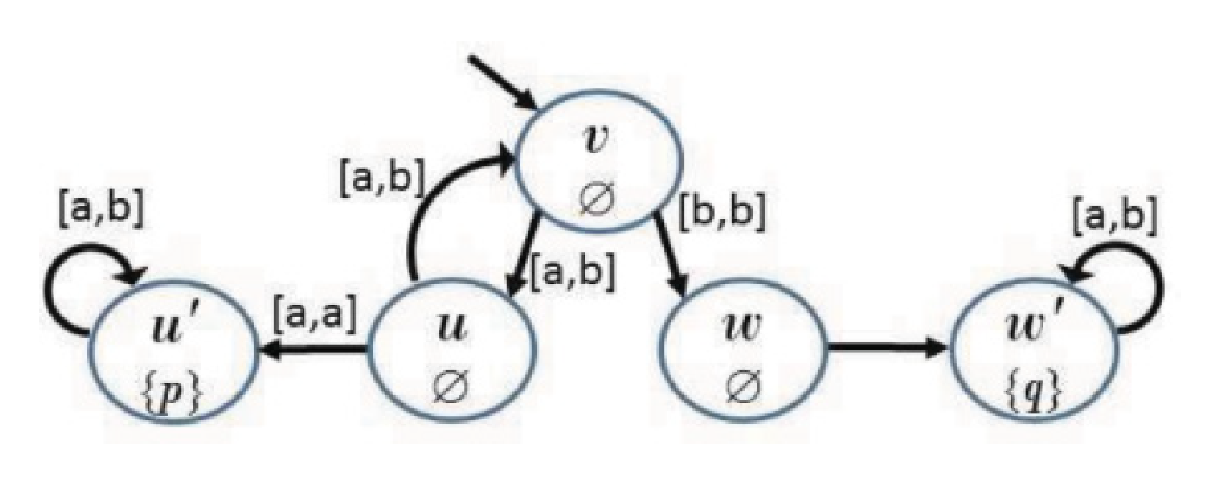
\epsfig{file=cg.eps,width=80mm} 
\end{center}
\caption{A concurrent game graph}
\label{fig.cg}
\end{figure} 
The ovals represent states while the arcs represent 
state transitions.  
We also put down the $\lambda$ values inside the corresponding states. 
On each edge, we label the tokens issued by the agents. 
Specifically, the label on arrow $(q,q')$ is 
$[\delta((q,q'),1),\ldots,\delta((q,q'),m)]$.  
For example, in Figure~\ref{fig.cg}, 
on edge $(v,u)$, we have label $[a,b]$ meaning that 
to make the transition, agent 1 has to choose token $a$ while 
agent 2 has to choose $b$.  

For convenience, in the remaining part of the manuscript, we assume that we are always in the context of a given game graph $\calg=\langle m,Q,r,P,\lambda,R,\Delta,\delta\rangle$.
Thus, when we write $Q,r,P,\lambda,R,\Delta$, and $\delta$ we respectively refer to the corresponding components of this $\calg$.  

A {\em state predicate} of $P$ is a Boolean combination of elements in $P$.
% We let $\emstp(P)$ be the set of state predicates of $P$.
The satisfaction of a state predicate $\eta$ at a state $q$,
in symbols $q\models \eta$, is defined in the standard way.

A {\em play} is an infinite path in a game graph.
A play is {\em initial} if it begins with the initial state.
Given a play $\rho=\bar{q}_0\bar{q}_1\ldots$,
for every $k\geq 0$, we let $\rho(k)=\bar{q}_k$.
Also, given $h\leq k$,
we let $\rho[h,k]$ denote $\rho(h)\ldots\rho(k)$ and
$\rho[h,\infty)$ denote the infinite tail of $\rho$
from $\rho(h)$.
A {\em play prefix} is a finite segment of a play from the beginning of
the play.
Given a play prefix $\rho=\bar{q}_0\bar{q}_1\ldots \bar{q}_n$, 
we use $|\rho|=n+1$ for the {\em length} of $\rho$.
For convenience, we use $\emlast(\rho)$ to denote the 
last state in $\rho$, i.e., $\rho(|\rho|-1)$.  

Let $Q^*$ be the set of finite sequences of states in $Q$.  
For an agent $a\in [1,m]$,
a {\em strategy} $\sigma$ for $a$ is
a function from $Q^*$ to $\Delta$.
An {\em agency} $A$ of $[1,m]$ is an integer subset of $[1,m]$.  
For example, ``$\{1,3,4\}$'' represents the agency that consists of agents 1, 3, and 4. 
A {\em strategy profile} (or {\em S-profile}) $\Sigma$ of 
an agency $A\subseteq [1,m]$ 
is a partial function from $[1,m]$ to the set of strategies
such that, for every $a\in[1,m]$, 
$a\in A$ iff %\footnote{``{\em iff}" is a shorthand for ``{\em if and only if}."} 
$\Sigma(a)$ is defined.  
The composition of two S-profiles $\Sigma,\Pi$,
in symbols $\Sigma\circ\Pi$, is defined with
the following restrictions for every $a\in[1,m]$.
\begin{list1}
\item If $\Pi(a)$ is defined,
    then $\Sigma\circ\Pi(a)=\Pi(a)$.
\item If $\Sigma(a)$ is defined and $\Pi(a)$ is undefined,
    then $\Sigma\circ\Pi(a)=\Sigma(a)$.
\item If $\Sigma(a)$ and $\Pi(a)$ are both undefined,
    then $\Sigma\circ\Pi(a)$ is also undefined.
\end{list1} 
% Later, w
We will use composition of S-profiles to model 
inheritance of strategy bindings from ancestor formulas. 

A play $\rho$ is compatible with a strategy
$\sigma$ of an agent $a\in [1,m]$
iff for every $k\in [0,\infty)$,
$\delta((\rho(k),\rho(k+1)),a)=\sigma(\rho[0,k])$.
The play is compatible with an S-profile $\Sigma$ of agency $A$ iff for every $a\in A$, the play is compatible with $\Sigma(a)$ of agent $a$.

\section{Turn-Based Games}
Another popular game structure is {\em turn-based game} in which at each state, at most one agent gets to decide the next state.
For example, in figure~\ref{fig.tg}, we have the graphical representation of a turn-based game graph with initial state $v$.
\begin{figure}[!ht]
\begin{center}
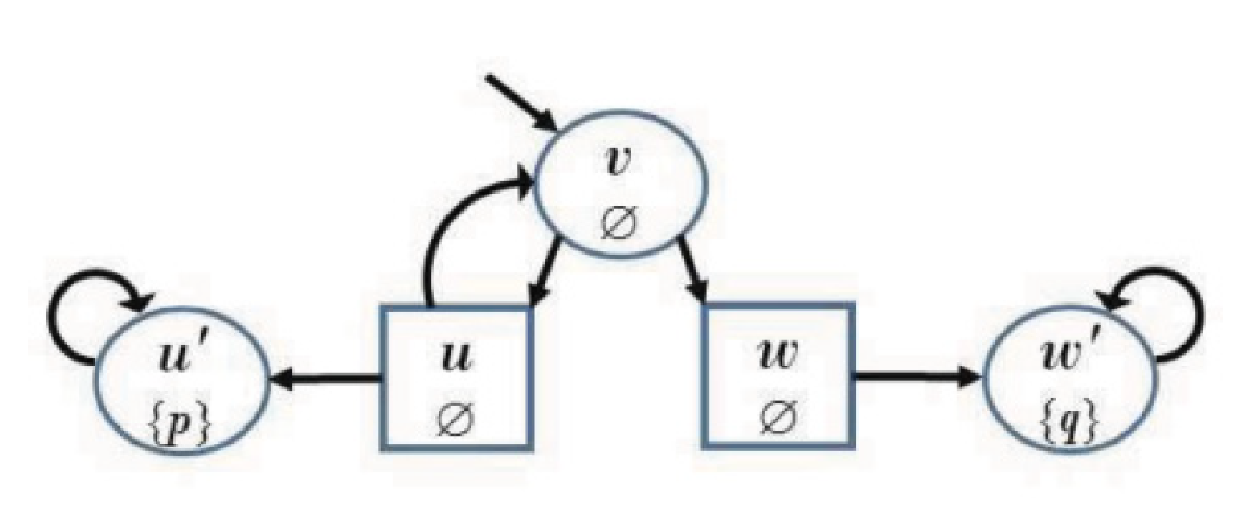
\epsfig{file=tg.eps,width=80mm} \\
$\bigcirc$ belongs to Agent 1 and $\pfrr$ belongs to Agent 2.
\end{center}
\caption{A turn-based game graph}
\label{fig.tg}
\end{figure} 
The ovals and squares represent states respectively of gent 1 and agent 2.
The arcs represent state transitions.  

In fact, every turn-based game can be represented as a special case of 
concurrent games.  
Specifically, a turn-based game 
$\calg=\langle m,Q,r,P,\lambda,E,\Delta,\delta\rangle$ 
can be viewed as a concurrent game with the following restrictions. 
\begin{list1} 
\item $\Delta=Q\cup\{\perp\}$ where $\perp$ denotes a dummy move not in $Q$. 
\item For every $(q,q')\in R$, if $q$ belongs to agent $a$, 
	then $\delta((q,q'),a)=q'$ and 
	for every $a'\neq a$, $\delta((q,q'),a')=\perp$. 
\item For every $(q_1,q_2),(q_3,q_4)\in R$ and agent $a$, 
	$\delta((q_1,q_2),a)=\perp$ if and only if $\delta((q_3,q_4),a)=\perp$.  
	This restriction says that every state can be owned by only one agent. 
\end{list1} 
For convenience, for a turn-based game, the owner of a state $q$, $\omega(q)$ in symbols, is defined as agent $a$ with $\forall (q,q')\in E(\delta((q,q'),a)=q'$.  
For ease of notation, we denote with $Q_a = \{q \in Q \mid \omega(q)=a\}$ the states owned by an agent $a$.

In the investigation of many research issues, turn-based game graphs are easier to handle than concurrent game graphs.   
So in latter sections, we sometimes use turn-based game graphs in examples and explanation of the theory as we see fit.

\section{Two-player concurrent game structures}
To facilitate the explanation of resilience analysis in a game's perspective, we start by defining a special case of the concurrent game, $\calk=\langle 2,Q,r,P,\lambda,R,E_1,E_2,\delta\rangle$.
The first difference is that there are only 2 players in the game.
For convenience, we divide the token set that player can choose, $\Delta$, into 2 subsets $E_1$ and $E_2$.
Intuitively, $E_1$ are the tokens set that can be picked by protagonist and $E_2$ are the tokens set that can be picked by antagonist.
Moreover, each member of $E_2$ are labelled by either $error$ or $non-error$ moves.

\section{Fault Tolerance}
Resilience to errors in computer systems is usually achieved through error recovery design as illustrated in Figure~\ref{fig.frwk}.  
\begin{figure}[t]
\begin{center}
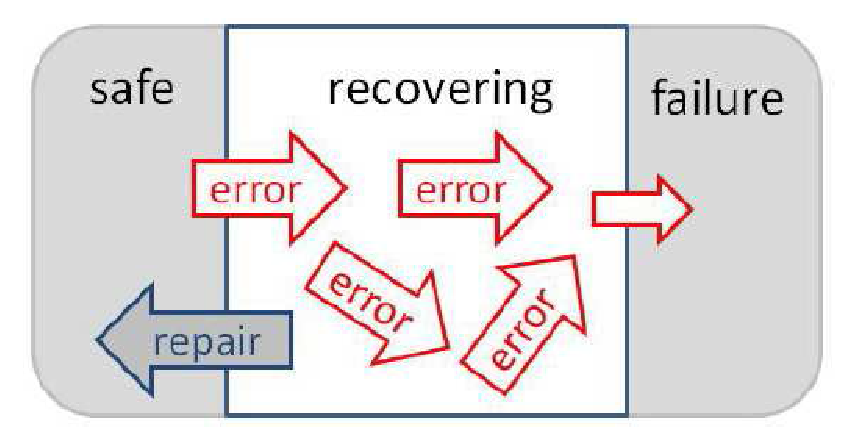
\epsfig{file=frwk.eps,width=60mm}
\caption{Framework of resilience design}
\label{fig.frwk} 
\end{center}
\end{figure}
The system states can be partitioned into three regions safe, recovery, and failure. 
The left part of the figure represents the safety region.
The states in this region represent those for 'normal' operation. 
When an error occurs, the system goes through a recovery process, in which it follows some recovery mechanism.
This is shown as the "recovering" area in Figure~\ref{fig.frwk}.
In this region, the system tries to repair the effects caused by an error and thus to go back to the safety region. 

In the recovery region, however, errors may still happen.
In general, fault-tolerant systems are built under the assumption that error detection and recovery is speedy and that there can only be a few errors during the process of recovery.
If the recovery mechanism is not resilient enough, a few errors may drive the system into failure.  

We use following 3 examples from computer architecture, OS interrupt handler and security system to illustrate our point. 

\begin{example} 
{\bf (Fault-tolerant computer architectures):}  
\label{exmp.avi}
In computer architectures, fault-tolerance is usually achieved via hardware duplication.  
Consider an example of a multi-processor system that includes $n$ processor copies and $m$ memory copies.  
The $n$ processors each can follow the instructions of the original system, or be engaged in memory recovery. 
When a copy of the memory fails, a processor can be assigned to recover it.
Majority check can be used to detect that a processor is faulty or that memory copy is faulty (often, both would happen at the same time).
For recovery, we can set a free processor to recover some memory copy, or make a processor follow the code of the majority of processors.

The key to error resilience is to decide whether to make a processor follow the execution of the majority, or to assign it to recover faulty memory.
If too many errors occur in a short while before the errors can be recovered from, then there may be no more processors left to carry out any more recovery. 
When such a critical situation arises, the system enters failure state when another error is induced.  

The recovery mechanism described above is typical in the design of fault-tolerant systems \cite{Pradhan96}.  
As explained, a practical recovery mechanism usually does not rely on the detailed structure of the system.  
Instead, error-detection techniques such as parity checks, voting (for majority checks), etc., are usually employed.  
In fact, the number of duplicates is usually critical to the resilience of the system to errors.
As long as the majority of the duplicate modules can be recovered in time (i.e., before the next wave of errors), resilience of the system can be achieved. 
\qed 
\end{example} 

\begin{example} {\bf (Exception handling):} 
\label{exmp.ehan} 
At the operating system level, errors are usually signalled via interrupt lines and handled with routines called handlers.
The first thing that needs to be done by a handler is to save the CPU state of the interrupted process.
In some operating systems, a static memory space is used for this purpose for each handler. 
In such a scheme, if the same error happens again while executing the error handler, then the system can run into the risk that the CPU states of the interrupted handler can be overwritten and destroyed. 

Another scheme is to use a stack to save the CPU states of the interrupted processes.  
Such a scheme seems resilient to errors that happen during the execution of error handlers.
Still, too many errors that happen during the execution of error handlers
can deny critical functions of the system and incur failures, including missed timer updates and priority inversions.
Thus, a proper assumption on the timely error recovery by the error handling routines is critical to the design of 
error resilience in such cases.
\qed 
\end{example} 

\begin{example} {\bf (Security attacks):}
\label{exmp.satt}
Security in the Internet also relies on resilience to attacks of hackers, viruses, malware, etc.  
For example, one common technique of attacks to communication modules is to overflow the communication buffers.  
In such attacks, the sizes of the buffers and the ability of the security procedures to detect and recover from such overflowing attacks is crucial to the resilience design.  
\qed 
\end{example} 

These examples show that recovery is a crucial concept for designing systems that are resilient to errors. 
When system errors are detected in such a system, the system activates a recovery mechanism to remove the effect of the errors.
When designing such systems, the system designers usually know what errors and failures the systems can expect, according to the specification.
To avoid failures in the occurrence of dense errors, the system designers usually incorporate many error recovery mechanism in the system, e.g., exception handlers and hardware/software redundancy. 
But, in general, it would be difficult for the designers to evaluate how effective their recovery mechanism is to dense errors.
To overcome this difficulty, we believe that it is important to support them with automated analytical tools with a solid foundation.

Resilience has also been used in \cite{EhlersT14,BloemEJK14} with a similar goal.
When synthesising code, one relies on assumptions of the behavior of the environment, and the formal specification would only ask for the provision of guarantees under the condition that the assumptions are satisfied.
When evaluating the quality of an implementation, the behavior in cases where the environment does not comply with the assumption matters.
In \cite{EhlersT14,BloemEJK14}, the resilience model we have introduced in the conference version \cite{HPSW/12/rapidRecovery} of this paper has been followed up upon, and proven to be well suited for reactive synthesis.

In this work, we use these observations to design a theoretical framework for synthesizing a control mechanism that provides the maximal resilience against software errors in a realistic error model.

 
\chapter{Basic Strategy-interaction Logic}
\label{c:bsil}

\section{Existed Logics about Game and Strategy}
\subsection{Prior to Strategy Logics}
\subsection{With Strategy Logics}

\section{Running Example}
\subsection{Trying to Write Down a Correct Formal Specification}
\subsection{Resorting to General Strategy Logics for a Correct Specification}
\subsection{BSIL: New Strategy Modalities Expressive Enough for the Specification}
\subsection{Symbolic Strategy Names and Path Obligations}
\subsection{Passing Down the Path Obligations While Observing the Restrictions Among S-Profiles}
\subsection{Finding Finite Satisfying Evidence for a Formula in a Computation Tree}

\section{Game Graphs}
\subsection{Concurrent Games}
\subsection{Turn-Based Games}


\section{BSIL}
\subsection{Syntax}
\subsection{semantics}
\subsection{ATL+}
\subsection{Memory}


\section{Expressive Power of BSIL}
\subsection{Comparison with GL}
\subsection{Comparison with AMC}
\subsubsection{Comparison with ATL*}

\section{Algorithm and Complexity}
\subsection{Computing Path Obligations and Passing Them Down the Computation Tree}
\subsection{Procedures for Checking BSIL Properties}
\subsection{Correctness Proof of the Algorithm}
\subsection{Complexities of the Algorithm}
\subsection{Lower Bound and Completeness}

\section{Automata for BSIL Model Checking}
\subsection{Alternating Automata}
\subsection{Model Checking with AAs}

\section{BSIL Satisfiability}

\section{Experiment}
\subsection{Implementation}
\subsection{Benchmarks and Their Experiment Report}
\subsection{Discussion of the Experiments}
\chapter{Temporal Cooperation Logic}
\section{TCL}
TCL is an extension of BSIL which allow SQs appear after temporal operators.
Thus, TCL is able to describe following complicate properties while BSIL is not.

Let's reuse the example of prisoner dilemma\ref{exmp.pd}.
We can specify that prisoner 1 has a {\em nice} strategy which means he will not betray other players until been betrayed in TCL by following expression.
\begin{center} 
\hfill 
$\langle 1\rangle \pfrr ((\langle+\rangle \nxt \neg\mbox{\tt betray}_1)
\vee \bigvee_{a\neq 1}\mbox{\tt betray}_a)$
\hfill (I) 
\end{center}

Similarly, we can describe more involved strategies, such as 'Prisoner 2 will always betray when she does not have the power to force Player 1 to always play nice.'
\begin{center} 
\hfill 
$\langle 2\rangle (
(\langle+\rangle \pfrr \mbox{\tt betray}_2) 
\vee \langle+\rangle\pfrr ((\langle+\rangle \nxt \neg\mbox{\tt betray}_1)
\vee \bigvee_{a\neq 1}\mbox{\tt betray}_a))$
\hfill (J) 
\end{center} 

Moreover, we can describe deterministic Nash equilibria like 'the three agents can cooperate such that every agent either eventually leaves prison, or stays forever in prison regardless of her own strategy under the current strategies of the remaining prisoners' in TCL.
\begin{center}
\hfill
$\langle 1,2,3\rangle
        \bigwedge_{a\in [1,3]}\big((
        \langle+\emptyset\rangle\pevt \neg \mbox{\tt jail}_a) \vee
        \langle-a\rangle \pfrr \mbox{\tt jail}_a\big)$
\hfill (K)
\end{center}


\subsection{Syntax}
A TCL formula $\phi$ is constructed with the following three syntax rules.
\smallskip

\noindent
% \begin{center}
$\begin{array}{rcl}
\phi    & ::= & p\;|\; \neg\phi_1 \;|\; \phi_1\vee \phi_2
    \;|\; \langle  A\rangle \psi
    \\
\psi  & ::= & \phi \;|\; \eta \;|\; \psi_1\vee \psi_2\;|\; \psi_1\wedge \psi_2
    \;|\; \langle+A\rangle \psi_1
    \;|\; \langle+A\rangle\nxt\psi_1 
    \;|\; \langle+A\rangle\eta_1\until \psi_1
    \;|\; \langle+A\rangle\psi_1\rmrel \eta_1 \\
    & | & \langle-A\rangle \psi_1
    \;|\; \langle-A\rangle\nxt\psi_1 
    \;|\; \langle-A\rangle\eta_1\until \psi_1
    \;|\; \langle-A\rangle\psi_1\rmrel \eta_1 
    \\
\eta  & ::= & \phi \;|\; \eta_1\vee \eta_2\;|\; \eta_1\wedge \eta_2
    \;|\; \langle+\rangle\nxt\eta_1 
    \;|\; \langle+\rangle\eta_1\until \eta_2
    \;|\; \langle+\rangle\eta_1\rmrel \eta_2 \\
    & | & \langle-A\rangle\nxt\eta_1 
    \;|\; \langle-A\rangle\eta_1\until \eta_2
    \;|\; \langle-A\rangle\eta_1\rmrel \eta_2 
\end{array}$
% \end{center}
\smallskip

Here, $p$ is an atomic proposition in $\calp$ and $A\subseteq \{1,\ldots,m\}$ is an agency.  
Property $\langle A\rangle\psi_1$ is an (existential) 
strategy quantification (SQ) specifying that
there exist strategies of the agents in $A$
that make all plays consistent with these strategies satisfy $\psi_1$.
Property $\langle+A\rangle\psi_1$ is an (existential) 
strategy interaction quantification (SIQ) and 
can only occur bound by an SQ.
Intuitively, $\langle+A\rangle\psi_1$ means that there exist strategies of the agents in $A$
that work with the strategies introduced by the ancestor formulas.
Likewise, $\langle -A \rangle$ indicates a revocation of the strategy binding for the agents in $A$.
$\langle + \rangle$ is an abbreviation for $\langle + \emptyset\rangle$ or, equivalently $\langle - \emptyset \rangle$.
Thus, it neither binds nor revokes the binding of the strategy of any agent.
Yet, it provides a temporalisation in that it provides a tree formula that can be interpreted at a particular point.

% For convenience, we call an SQ also as an SIQ that interacts with 
% no ancestor formula strategies. 

`$\until$' is the {\em until} operator.  
The property $\psi_1\until\psi_2$ specifies a play along which 
$\psi_1$ is true until $\psi_2$ becomes true.  
Moreover, along the play, $\psi_2$ must eventually be fulfilled.   
`$\rmrel$' is the {\em release} operator.  
Property $\psi_1\rmrel\psi_2$ specifies a play along which either 
$\psi_2$ is always true or $\psi_2\until(\psi_1\wedge\psi_2)$ 
is satisfied. (Release is dual to until: $\neg(\phi_1 \until \phi_2) \, \Leftrightarrow \, \neg \phi_2 \rmrel \neg \phi_1$.)

In the following we may use $\langle?A\rangle\psi$ to conveniently 
denote an SQ or SIQ formula with `$?$' is empty, `+', or `-'.  
An SIQ $\langle\pm A\rangle\psi$ is called non-trivial if 
$A$ is not empty, and trivial otherwise. 

Formulas $\phi$ are called {\em TCL} {\em formulas}, {\em sentences}, or 
{\em state formulas}.  
Formulas $\psi$ and $\eta$ are called {\em tree formulas}.  
Note that we strictly require that non-trivial strategy interaction cannot 
cross path modal operators.  
This restriction is important because it offers a sufficient level of locality to efficiently model-check a system against a TCL property.
To illustrate this and to provide a simple extension that offers more expressive power to the cost of a much higher complexity, we informally discuss a small extension,
\emph{extended TCL} (ETCL), where the production rule of $\psi$ also contains $\neg \psi$ and show that it can be used to encode ATL$^*$, and the realisability problem of prenex QPTL can be reduced to ETCL model-checking.

%  and allows us to analyse the interaction 
% of strategies locally in a state and 
% then enforce the interaction along all paths from the state.  


For convenience, we also have the following shorthand notations.
\begin{center}
$\begin{array}{rclcrcl}
\true
& \equiv & p\vee(\neg p) 
& \hspace*{10mm} & % \\
\false
& \equiv & \neg\true \\
\phi_1\wedge \phi_2
& \equiv & \neg((\neg\phi_1)\vee(\neg\phi_2)) 
& \hspace*{10mm} & % \\
\phi_1\Rightarrow \phi_2
& \equiv & (\neg \phi_1)\vee \phi_2 \\
\pevt \phi_1
& \equiv & \true\,\until \phi_1 
& \hspace*{10mm} & % \\
\pfrr \phi_1
& \equiv & \false\,\rmrel \phi_1 \\
% \neg\psi_1\until\psi_2
% & \equiv & \psi_1\rmrel \psi_2 
% & \hspace*{10mm} & % \\
% \neg\psi_1\rmrel\psi_2
% & \equiv & \psi_1\until \psi_2 \\
\neg\nxt \phi_1
& \equiv & \nxt\neg\phi_1 
& \hspace*{10mm} & % \\
\; \langle A\rangle \nxt\psi_1 
& \equiv & \langle A\rangle \langle+\rangle\nxt\psi_1 \\
\; \langle A\rangle \psi_1\until\psi_2
& \equiv & \langle A\rangle\langle+\rangle \psi_1\until\psi_2 
& \hspace*{10mm} & % \\
\; \langle A\rangle \psi_1\rmrel\psi_2  
& \equiv & \langle A\rangle \langle+\rangle\psi_1 \rmrel\psi_2 \\
% & \hspace*{10mm} & % \\
% \; \langle A\rangle \psi_1\until\psi_2
% & \equiv & \langle A\rangle\langle+\rangle \psi_1\until\psi_2 \\
\end{array}
$
\end{center} 
In general, it would also be nice to have the universal SQs and 
SIQs as duals of existential SQs and SIQs, respectively. 
Couldn't we add, or encode by pushing negations to state formulas, 
a property of the form $[+A]\psi_1$, meaning that, for all strategies of agency $A$,  $\psi_1$ will be fulfilled? 
In principle, this is indeed no problem, and extending the semantics would be simple.
This logic would be equivalent to allowing for negations in the production rule of $\psi$.
The problem with this logic is that it is too succinct.
We will briefly discuss in the following section that model-checking becomes non-elementary if we allow for such negations.

% Note, however, that an introduction of negations in the production rule of $\eta$ is only notational sugar.
% As the SIQs in the $\eta$ production rule do not introduce strategies, they are self-dual, and negations can be pushed inside.
% (Cf.\ example (E) from the introduction, where the left hand side of implication can be replaced by
% $( \langle+\emptyset\rangle\pevt \neg \mbox{\tt jail}_a)
% \vee \langle-a\rangle \pfrr \mbox{\tt jail}_a$.)

% All TCL formulas are {\em well-formed} 
% since all their SIQs occur inside
% an SQ beginning with $\langle  A\rangle$
% for some $A$.

From now on, we assume that we are always in the context of a
given TCL sentence. % $\chi$.  
\subsection{semantics}
In order to prepare the definition of a semantics for TCL formulas, 
we start with the definition of a semantics for sentences 
of the form $\langle A \rangle \psi$, where $\psi$ does not contain any SQs.
We call these formulas \emph{primitive} TCL formulas.

Due to the design of TCL, strategy bindings can only effectively happen at non-trivial SQs $\langle A \rangle$ and 
when a non-trivial SIQ $\langle +B\rangle$ is interpreted.
% Moreover, for a subformula $\psi_1\until\psi_2$ 
% (or $\psi_1\rmrel\psi_2$), there is no new strategy binding in 
% $\psi$ to interact with those bound to $\psi_1\until\psi_2$ 
% (or $\psi_1\rmrel\psi_2$).  
%
To ease referring to these strategies, we first define the \emph{bound agency} of a subformulas $\phi$ of a TCL sentence $\chi$, denoted $\embnd(\phi)$, as follows.
\begin{list1} 
\item For state formulas $\phi$, $\embnd(\phi)= \emptyset$.  
\item For state formulas $\langle A \rangle \psi$,  $\embnd(\psi)= A$ (unless $\psi$ is a state formula).
\item For tree formulas $\psi_1=\langle +A \rangle \psi_2$,  $\embnd(\psi_2) = \embnd(\psi_1) \cup A$.
\item For tree formulas $\psi_1=\langle -A \rangle \psi_2$,  $\embnd(\psi_2) = \embnd(\psi_1) \smallsetminus A$.
\item For all other tree formulas $\psi_1$ or $\psi_2$ with $\psi = \psi_1 \mathsf{OP} \psi_2$, with $\mathsf{OP} \in \{\wedge,\vee,\mathcal U, \mathcal R\}$, we have $\embnd(\psi_1) = \embnd(\psi)$ or $\embnd(\psi_2) = \embnd(\psi)$, respectively.
\end{list1} 
$\embnd$ shows, which agents have strategies assigned to them 
by an SIQ or SQ.
Note that this leaves the $\embnd$ undefined for all state formulas not in the scope of an SQ formulas.
For completeness, we could define $\embnd$ as empty in these cases, but a definition will not be required in the definition of the semantics.

As the introduction of additional strategies through non-trivial SIQ $\langle +B\rangle$ is governed by a \emph{positive} 
Boolean combination, all strategy selections can be performed concurrently.
Such a design leads us to the concept of strategy schemes.

A {\em strategy scheme} $\sigma$ is the set of strategies introduced by any non-trivial SQ $\langle A \rangle$ or SIQ $\langle + A \rangle$.
By abuse of notation, we use $\sigma[\phi,a]$ to identify such a strategy.
Read in this way, $\sigma$ can be viewed as a partial function from subformulas and their bound agencies to strategies.
Thus, $\sigma[\phi,a]$ is defined if $a\in \embnd(\phi)$ is in the bound agency of $\phi$.

% The SIQ or SQ operator introducing a strategy for $a$ can be found by walking up the formula tree, starting at $\phi$, and stopping once a formula $\psi$ starting with $\langle A \rangle$ or $\langle + A \rangle$ with $a\in A$ is hit.
% $\sigma[\phi,a]$ refers to the strategy for Agent $a$ introduced by this quantifier.

For example, given a strategy scheme $\sigma$ for a 
TCL sentence $\langle 1\rangle \pevt ((\langle+2\rangle \nxt p)\wedge\langle 2\rangle\pfrr q)$, 
the strategy used in $\sigma$ by Agent $1$ to enforce 
the whole formula can be referred to by
\[\sigma[\langle 1\rangle \pevt ((\langle+2\rangle \nxt p)\wedge\langle 2\rangle\pfrr q),1],\]
but also by $\sigma[\langle+2\rangle \nxt p,1]$, while $\sigma[\langle 2\rangle\pfrr q,1]$ is undefined.
% the one to enforce $\langle+2\rangle \nxt p$ by Agent $2$ is 
% named $\sigma[\langle+2\rangle \nxt p,2]$.  


We use a simple tree semantics for TCL formulas. 
A (computation) tree $T_r$ is obtained by unravelling $\calg$ from $r$  
and expand the ownership 
and labelling functions from $\calg$ to $T_r$ in the natural way.
Technically, we have the following definition.  

\paragraph{\bf Definition: Computation Tree.} 
A {\em computation tree} for a turn based game $\calg$ from a state $q$, 
denoted $T_q$, is the smallest set of play prefixes that contains $q$ and, for all $\pi\in T$ and $(\emlast(\pi),q')\in \cale$, $\pi q'\in T$.
\qed 


The {\em strategy-pruned} tree for a tree node $\pi$, 
a strategy scheme $\sigma$,
and a subformula $\psi_1$ of $\chi$ from a state $q$, 
in symbols $T_q\langle\pi,\sigma,\psi_1\rangle$, 
is the smallest subset of $T_q$ such that: 
\begin{list1} 
\item $\pi\in T_q\langle\pi,\sigma,\psi_1\rangle$;  
\item for all $\pi' \in T_q\langle\pi,\sigma,\psi_1\rangle$ 
  with $\omega\big((\emlast(\pi')\big)\notin\embnd(\psi_1)$ 
  and $(\emlast(\pi'),q')\in \cale$, 
  $\pi' q'\in T_q\langle\pi,\sigma,\psi_1\rangle$;  
\item for all $\pi' \in T_q\langle\pi,\sigma,\psi_1\rangle$,  
  $a=\omega\big((\emlast(\pi')\big)$, and 
  $q'=\sigma[\psi_1,a](\pi')$ 
  with $a\in\embnd(\psi_1)$, 
%   $(\emlast(\pi),q') \in \cale$ and 
  $\pi' q' \in T_q\langle\pi,\sigma,\psi_1\rangle$.
\end{list1}
Given a computation tree or a strategy-pruned tree $T$ and a node $\pi\in T$, 
for every $\pi q\in T$, we say that $\pi q$ is a successor of $\pi$ in $T$. 
A play $\rho$ is a \emph{limit of $T$} (or an infinite path in $T$), in symbols $\rho\stackrel{\infty}\in T$, 
if there are infinitely many prefixes of $\rho$ in $T$. 


We now define the semantics of subformulas of primitive TCL formulas 
inductively as follows.  
Given the computation tree $T_q$ of $\calg$, a tree node $\pi\in T_q$, 
and a strategy scheme $\sigma$, 
we write $T_q,\pi,\sigma\models\psi_1$ to denote that 
$T_q$ satisfies $\psi_1$ at node $\pi$ with strategy scheme $\sigma$.

While the notation might seem heavy on first glance, note that the truth for state formulas merely depends on the state $\emlast(\pi)$ in which they are interpreted, and the tree formulas are simply interpreted on a strategy pruned tree rooted in $\pi$ and defined by the strategy scheme.
\begin{list1}
\item For state formulas $\phi$ other than SQ formulas,
  we use the state formula semantics:
$T_q,\pi,\sigma\models \phi$ iff $\calg,\emlast(\pi) \models \phi$, 
with the usual definition.  
\begin{list2}
\item  $\calg,q \models p$ if, and only if, $p\in\lambda(q)$,
\item  $\calg,q \models \neg \phi$ if, and only if, $\calg,q \not\models \phi$,
\item  $\calg,q \models \phi_1 \vee \phi_2$ if, and only if, $\calg,q \models \phi_1$ or $\calg,q \models \phi_2$, and
\item  $\calg,q \models \phi_1 \wedge \phi_2$ if, and only if, $\calg,q \models \phi_1$ and $\calg,q \models \phi_2$.
\end{list2}
(Note that this allows for using negation for state formulas.)

\item $T_q,\pi,\sigma \models \psi_1\vee\psi_2$ iff
    $T_q,\pi,\sigma \models \psi_1$
    or $T_q,\pi,\sigma \models \psi_2$.
     \mbox{(The $\psi_i$ are no state formulas.)}
\item $T_q,\pi,\sigma\models \psi_1\wedge\psi_2$ iff
    $T_q,\pi,\sigma\models \psi_1$
    and $T_q,\pi,\sigma\models \psi_2$ hold.
    
\item $T_q,\pi,\sigma\models \langle \pm A \rangle \nxt \psi$ iff,
     for all successors $\pi q'$ of $\pi$ 
     in $T_q\langle \pi,\sigma,\langle \pm A \rangle\nxt\psi_1\rangle$, 
     $T_q,\pi q',\sigma \models \psi$ holds.  
    
\item $T_q,\pi,\sigma \models \langle \pm A \rangle \psi_1\until\psi_2$ iff, for all limits 
    $\rho\stackrel{\infty}\in T_q\langle \pi,\sigma, \langle \pm A \rangle\psi_1\until\psi_2\rangle$, 
    there is a $k \geq |\pi|-1$ 
    such that $T_q,\rho[0,k],\sigma \models \psi_2$ and, 
    for all $h\in [|\pi|-1,k-1]$, 
    $T_q,\rho[0,h],\sigma\models \psi_1$ hold. 
\item $T_q,\pi,\sigma \models \langle \pm A \rangle \psi_1\rmrel\psi_2$ iff, 
    for all limits 
    $\rho\stackrel{\infty}\in T_q\langle\pi,\sigma,\langle \pm A \rangle\psi_1\rmrel\psi_2\rangle$, one of the following two restrictions 
    are satisfied. 
    \begin{list2} 
    \item For all $k \geq |\pi|-1$, $T_q,\rho[0,k],\sigma \models \psi_2$. 
    \item There is a $k\geq |\pi|-1$ such that 
      $T_q,\rho[0,k],\sigma\models \psi_1\wedge\psi_2$, and, 
      for all $h\in [|\pi|-1,k]$, $T_q,\rho[0,h],\sigma\models \psi_2$.
    \end{list2} 
\item $T_q,\pi,\sigma\models \langle \pm A \rangle \psi_1$ iff
    $T_q,\pi,\sigma \models \psi_1$.
\item $\calg, q \models \langle A \rangle \psi_1$ iff there is a strategy scheme $\sigma$ such that
    $T_q,q,\sigma \models \psi_1$.
\end{list1}

If $\phi_1$ is a TCL sentence %and $T_q,q,\sigma\models\phi_1$ 
% for some strategy scheme $\sigma$,
% then we may simply write $\calg,q\models\phi_1$.  
% If
then we write $\calg\models\phi_1$ for $\calg,r\models\phi_1$.


Note that, while asking for the existence of a strategy scheme refers to all strategies introduced by some SQ or SIQ in the TCL sentence, only the strategies introduced by the respective SQ and the SIQs in its scope are relevant.

The simplicity of the semantics is owed to the fact that 
it suffices to introduce new strategies at the points 
where eventualities become true for the first time.
Thus, they do not really depend on the position 
in which they are invoked and we can guess them up-front. 
(Or, similarly, together with the points on the unravelling 
where they are invoked.)
%
This is possible, simply because the validity of state formulas (and hence of TCL sentences) cannot depend on the validity of the left hand side of an until (or the right hand side of a release) \emph{after} the first time it has been satisfied. 


\section{Expressive Power of TCL}
Note that TCL is not a superclass of BSIL since 
BSIL allows for negation in front of SIQs while TCL does not. 
However, by examining the proofs in \cite{WHY11} 
for the inexpressibility of BSIL properties by ATL$^*$, GL, and AMC, 
we find that the BSIL sentence used in the proofs is also a TCL sentence. 
This leads to the conclusion that 
there are properties expressible in TCL but cannot 
be expressed in ATL$^*$, GL, and AMC.  

{\lemma \label{lemma.express.incomp1} 
There are TCL sentences that cannot be expressed 
in any of ATL$^*$, GL, or AMC.  
} 
\qed 


TCL is, in fact, not only a powerful logic, 
but also contains important logics either as syntactical fragments or can embed them in a straight forward way.
ATL and CTL can be viewed as syntactic fragments of TCL.

But it is also simple to embed LTL and even CTL$^*$.
We start with $\exists$LTL, the less used variant 
where one is content if one path satisfies the formula.
% Let $A$ denote the set of all agents.
We then translate an LTL formula, which we assume w.l.o.g.\ 
to be in negative normal form 
(negations only in front of atomic propositions).
Then ``there is a path that satisfies $\phi$'' is equivalent to
$\langle 1,\ldots,m \rangle \widehat{\phi}$, where $\widehat{\phi}$ is derived from $\phi$ by replacing every occurrence of $\nxt$, $\until$, and $\rmrel$ by
$\langle + \rangle \nxt$, $\langle + \rangle \until$, and $\langle + \rangle \rmrel$, respectively.
%
The simple translation is possible because the formula $\widehat{\psi}$ 
is de-facto interpreted over a path, 
the path formed by the joint strategy of the agency $[1,m]$.
The $\langle + \rangle$ operators we have added have no effect on the semantics in such a case, just as a CTL formula can be interpreted as the LTL formula obtained by deleting all path quantifiers when interpreted over a word.

Consequently, we have the expected semantics for $\forall LTL$:  ``all paths satisfy $\phi$'' is equivalent to
$\neg \langle A \rangle \widehat{\neg\phi}$, where $\neg \phi$ is assumed to be re-written in negative normal form.
% This immediately implies that TCL model-checking is PSPACE hard.
% 
The encoding of $\exists$LTL and $\forall$LTL can easily be extended to the encoding of CTL$^*$.  
%
{\lemma \label{lemma.express.ctl.star}
TCL is more expressive than CTL$^*$ and LTL.  
}
\qed 

This encoding does not extend to ATL$^*$.
$\langle 1\rangle ((\pfrr p)\vee \pfrr q)$  is an ATL$^*$ property that cannot be 
expressed with TCL.

This is different from the 
% \begin{center} 
ATL property $(\langle 1\rangle \pfrr p)\vee \langle 1\rangle\pfrr q$ 
% \end{center} 
or the
% \begin{center} 
TCL property
\mbox{$\langle 1\rangle ((\langle+\rangle\pfrr p)\vee \langle +\rangle\pfrr q)$}. 
% \end{center} 
In fact, the proofs and examples in \cite{WHY11} 
can also be applied in this work to show that 
there are properties of ATL$^*$ (or GL, or AMC) 
that cannot be expressed with TCL.  
This leads to the following lemma. 

{\lemma \label{lemma.express.incomp2} 
TCL is incomparable in expressiveness with ATL$^*$, GL, and AMC.  
} 
\qed 

Note, however, that allowing for a negation in the definition of $\psi$ would change the situation.
Then an ATL$^*$ formula $\langle A \rangle \psi$ 
(assuming for the sake of simplicity that $\psi$ is an LTL formula), 
would become
$\langle A \rangle \neg \langle + [1,m] \smallsetminus A \rangle \widehat{\neg \psi}$ in the extended version of TCL.
The translation extends to full ATL$^*$, but this example also demonstrates why negation is banned: even without nesting, we can, by encoding ATL$^*$, encode a 2EXPTIME complete model-checking problem, losing the appealing tractability of our logic.

In fact, it is easy to reduce the realisability problem of prenex QPTL, and hence a non-elementary problem, to the model-checking problem of extended TCL.
Using the game structure from Figure \ref{fig.nonelementary}, we can encode the realisability of a prenex QPTL formula with $n-1$ variables, for simplicity of the form
$\forall p_2 \exists p_3 \forall p_4 \ldots \exists p_n \phi$, where $p_2,\ldots,p_n$ are all propositions occurring in $\phi$.
We reduce this to model-checking the formula 
\[\phi'=\langle 1 \rangle \neg \langle +2 \rangle \neg \langle +3 \rangle \neg \langle +4 \rangle \neg \ldots \neg \langle +n \rangle (\psi_\phi \wedge \langle + \rangle \pfrr p_1),\]
where $\psi_\phi$ can be obtained from $\widehat{\phi}$ by replacing
\begin{list1}
\item every literal $p_i$ by $\langle - 1 \rangle \langle + 1 \rangle \nxt (p_i \wedge \langle + \rangle \nxt p_i)$, and
\item every literal $\neg p_i$ by $\langle - 1 \rangle \langle + 1 \rangle \nxt (p_i \wedge \langle + \rangle \nxt \neg p_i)$.
\end{list1}

These formulas are technically not extended TCL formulas as $\langle +i \rangle \psi_1$ is not part of the production rule of $\psi$,  but $\langle +i \rangle \psi_1$ can be used as an abbreviation for $\langle +i \rangle \false \until \psi_1$.

Checking satisfiability of $\phi$ is is equivalent to model-checking $\phi'$ on the game shown in Figure \ref{fig.nonelementary}. 
The game has $n+1$ nodes, agents, and atomic propositions.
The nodes in Figure \ref{fig.nonelementary} are labeled with the agent that owned the nodes, and the atomic proposition $p_i$ is true exactly in node $i$.
From his state, Agent $1$ can move to any other state, 
while all other agents can either stay in their state or return 
to the state owned by Agent $1$.

The game starts in the node owned by Agent $1$, and in order to comply with the specification, the outermost strategy profile chosen by Agent $1$ must be to stay in the initial state for ever.
$\psi_\phi$ is chosen to align the truth of $p_i$ at position $j \in \mathbb N$ with the decision that Agent $i$ makes on the history $1^j i$: $\true$ corresponds to staying in $i$ and $\false$ with returning to $1$.

\begin{figure}[t]
{
\begin{center}
\psset{xunit=2cm,yunit=-1cm}
\begin{pspicture}(0,0)(5,1.2)
\tiny
\pnode(2.25,0){1}
\rput(2.5,0){\circlenode{0}{$1$}}

\ncline{->}{1}{0}

\rput(0,1){\circlenode{1}{$2$}}
\rput(1,1){\circlenode{2}{$3$}}
\rput(2,1){\circlenode{3}{$4$}}
\rput(3,1){\circlenode{4}{$5$}}
\rput(4,1){$\cdots$}
\rput(5,1){\circlenode{5}{$n$}}

\ncline{<->}{0}{1}
\ncline{<->}{0}{2}
\ncline{<->}{0}{3}
\ncline{<->}{0}{4}
\ncline{<->}{0}{5}

\nccircle[angleA=0]{->}{0}{.18}
\nccircle[angleA=180]{->}{1}{.18}
\nccircle[angleA=180]{->}{2}{.18}
\nccircle[angleA=180]{->}{3}{.18}
\nccircle[angleA=180]{->}{4}{.18}
\nccircle[angleA=180]{->}{5}{.18}

\end{pspicture}
\end{center}
}
\caption{The turn-based game graph from the non-elementary hardness proof of extended TCL.}
\label{fig.nonelementary}
\end{figure} 

It is not hard to establish a matching upper bound for model-checking extended~TCL.

\section{Complexity of TCL\label{sec.gen.proc}} 

In this section, we show that model-checking TCL formulas is EXPTIME-complete in the formula and P-complete in the model (and for fixed formulas), while the satisfiability problem is 2EXPTIME-complete.
As the proof of inclusion of the satisfiability problem in 2EXPTIME builds on the proof of the inclusion of model-checking in EXPTIME, we start with an outline of the EXPTIME hardness argument for the TCL model-checking problem and then continue with describing EXPTIME and 2EXPTIME decision procedures for the TCL model and satisfiability checking problem, respectively.
2EXPTIME hardness for TCL satisfiability is implied by the inclusion of CTL* as a de-facto sub-language \cite{Vardi+Stockmeyer/85/CTL}.



We show EXPTIME hardness by a reduction from 
the {\sf PEEK-$G_6$}~\cite{SC79} game.
An instance of {\sf PEEK-$G_6$} consists of 
two disjoint sets of boolean variables, 
$P_1=\{p_1,\ldots,p_h\}$ (owned by a safety agent) and 
$P_2=\{p_{h+1},\ldots,p_{h+k}\}$ (owned by a reachability agent), 
a subset $I\subseteq P_1\cup P_2$ of them that are initially {\em true}, 
and a boolean formula $\gamma$ in CNF over 
$P_1\cup P_2$ that the reachability agent wants to become 
{\em true} eventually.
The game is played in turns between the safety and the reachability agent 
(say, with the safety agent moving first), and 
each player can change the truth value of one of his or her variables 
in his/her turn.

\begin{lemma}
\label{lemma.exptime.hard}
TCL model-checking is EXPTIME hard for primitive TCL formulas.
\end{lemma}

\begin{proof}
To reduce determining the winner of an instance of a {\sf PEEK-$G_6$} game to TCL model-checking, 
we introduce a 2-agent game $\calg=\langle 2,\calq,r,\omega,\calp,\lambda,\cale\rangle$ 
as shown in Figure \ref{fig.exptime}, where Agent 1 (he, for convenience) represents the safety agent 
while Agent 2 (she, for convenience) represents the reachability agent.
$t_{h+k}$ and $f_{h+k}$ are the only states owned by Agent 2.

\begin{figure}[t]
{
\begin{center}
\psset{xunit=2cm,yunit=1cm}
\begin{pspicture}(0,-.7)(5,1.7)
\tiny
\pnode(-.25,0.5){0}
\rput(0,0.5){\circlenode{r}{$r$}}

\rput(1,0){\circlenode{t1}{$f_1$}}
\rput(1,1){\circlenode{f1}{$t_1$}}

\rput(2,0){\circlenode{t2}{$f_2$}}
\rput(2,1){\circlenode{f2}{$t_2$}}

\rput(3,0){\circlenode{t3}{$f_3$}}
\rput(3,1){\circlenode{f3}{$t_3$}}

\ncline{->}{0}{r}
\ncline{->}{r}{t1}
\ncline{->}{r}{f1}

\ncline{->}{t1}{t2}
\ncline{->}{t1}{f2}
\ncline{->}{f1}{t2}
\ncline{->}{f1}{f2}

\ncline{->}{t2}{t3}
\ncline{->}{t2}{f3}
\ncline{->}{f2}{t3}
\ncline{->}{f2}{f3}

\rput(3.5,0.5){$\cdots$}

\rput(4,0){\rnode{t1}{\psframebox[framesep=4pt]{$f_{h+k}$}}}
\rput(4,1){\rnode{f1}{\psframebox[framesep=4pt]{$t_{h+k}$}}}

\rput(5,-.5){\circlenode{t2}{$1$}}
\rput(5,0.5){$\vdots$}
\rput(5,1.5){\circlenode{f2}{$k$}}

\ncline{->}{t1}{t2}
\ncline{->}{t1}{f2}
\ncline{->}{f1}{t2}
\ncline{->}{f1}{f2}

\ncarc[arcangle=-20.5]{->}{f2}{r}
\ncarc[arcangle=20.5]{->}{t2}{r}

\end{pspicture}
\end{center}
}
\caption{The turn-based game graph from the EXPTIME hardness proof.}
\label{fig.exptime}
\end{figure} 

The game is played in rounds, and a round starts each time the game is at state $r$.
If the game goes through $t_i$ this is identified with the variable $p_i$ to be true.
Likewise, going through $f_i$ is identified with the variable being false.

It is simple to write a TCL specification that forces the safety player to toggle the value of exactly one of his variables in each round, and to toggle the value of the variable $p_{h+i}$ of the reachability player defined by the state $i$ she has previously moved to, while maintaining all other variable values.
Requiring additionally that the safety agent can guarantee that the boolean formula is never satisfied provides the reduction.
\qed
\end{proof}

The details of the construction are available in the full version. 
It is interesting that a game with only two agents suffices for the proof.  
Two agents are also sufficient to show P hardness for fixed formulas, as solving a reachability problem for AND-OR graphs \cite{Immerman81} naturally reduces to showing $\langle 1 \rangle \pevt p$.

\begin{lemma}
\label{lemma.nl.hard}
TCL model-checking for fixed formulas is P hard for primitive TCL formulas.
\qed 
\end{lemma}

In order to establish inclusion in EXPTIME and P, respectively, we use an automata based argument.

\begin{theorem}
\label{theo.ms.complete}
The model-checking problem of TCL formulas against turn-based game graphs
is EXPTIME-complete, and P-complete for fixed formulas.
\end{theorem}

\begin{proof}
We first show the claim for primitive TCL formulas $\phi=\langle A \rangle \psi$.
 
To keep the proof simple, we first consider a tree automaton $\mathcal U$ that checks the acceptance of $\psi$ for a given strategy scheme $\sigma$.
That is, $\mathcal U$ checks if ${T_q}^+,q,\sigma \models \psi$ under the assumption that both $\sigma$ and the truth values for the subformulas starting with a $\langle \pm B \rangle$ are encoded in the nodes of ${T_q}^+$.

Such an automaton would merely have to run simple consistency checks, and it is simple to construct a suitable universal weak tree automaton $\mathcal U$, which is polynomial in the size of $\phi$.
From there it is simple to infer a deterministic B\"uchi tree automaton 
$\mathcal D$, which is exponential in the weak universal tree automaton 
\cite{Muller+Schupp/95/Alternating}.

It is then a trivial step (projection) to \emph{guess} $\sigma$ and the truth annotation of the subformulas on the fly, turning the deterministic B\"uchi tree automaton $\mathcal D$ that requires a correct annotation into a nondeterministic B\"uchi automaton $\mathcal N$ of the same size that checks $\calg,q \models \phi$.
%
Acceptance can be checked in time quadratic in the size of the product of $\mathcal N$ and $\calg$ \cite{Chatterjee+Henzinger/12/Buchi}.

To take the step to full TCL, we can model-check the truth of primitive TCL formulas and then use the result of this model-checking instead of the respective subformula.

Hardness is inherited from Lemmata \ref{lemma.exptime.hard} and \ref{lemma.nl.hard}.
\qed
\end{proof}

This argument shows more: the complexity of TCL model-checking for fixed formulas does not depend on the formula.
It suffices to solve a number of B\"uchi games, where both the size of the game and the number of games to be played is linear in $\mathcal G$.

\begin{corollary}
Viewing the size of a TCL sentence as a parameter, TCL model-checking is fixed parameter tractable.
\end{corollary}

The automata construction from the proof of Theorem \ref{theo.ms.complete} extends to a construction for satisfiability checking.


\chapter{Software Resilience against Dense Errors}
\label{c:resilience}

\section{Resilience in a Nutshell}
From Example~\ref{exmp.avi} to \ref{exmp.satt} in the previous section, it is easy to see the common paradigm of error recovery in software systems.  

\begin{quote}
When errors are detected, a recovery mechanism will be activated to avoid failures and try to get back to normal execution. 
\end{quote}

Moreover, such a recovery mechanism usually needs to operate under the assumption that more errors may also happen during the recovery process.
In practice, system designers have already implemented many defensive modules, e.g., exception handlers, which are certainly good candidates for the recovery segments.  
Thus, the recovery scheme we discuss is likely to have arisen in an ad-hoc fashion as a natural concept when software architects and programmers designed recovery mechanisms for critical software.  

The vast state spaces of critical systems make an automated support for and a solid foundation of evaluating design alternatives particularly valuable. 

In the following, we will use the examples from the previous subsection as a motivation for defining a new game, called {\em safety resilience game}, between the recovery mechanism (the protagonist) and the error-injecting agent (the antagonist).  
The game is specified with a set $F$ of failure states, a set $S$ of safe states (the safety region), the moves by the antagonist to inject errors, and the resilience level $k$ that the designers want to achieve. 
The objective of the protagonist is to identify a control strategy so that the whole system can achieve the prescribed level (or the highest level) $k$ of resilience for safety region $S$ (a set of states) and failure state set $F$.  

The game is played round by round. 
When the antagonist issues an error move, 
the play may be deflected into a recovery segment.  
If there are no more than $k-1$ errors in the recovery segment, 
then a $k$-resilient control mechanism must direct the recovery segment
to end at a safe state. 
The above observation suggests that 
a safety region can be abstracted as a fixed point 
to the recovery procedure 
that transforms a safe state to another safe state via the recovery segment 
with at most $k-1$ errors. 
Conceptually, a fixed point to a procedure $f(x)$ is a set $S$ of elements 
in the domain of $x$ such that $S=\{f(x)\mid x\in S\}$.  
To calculate the fixed point of the recovery procedure, 
we can use the greatest fixed point algorithm.  
The idea is to start from a superset of the recovery procedure fixed point. 
For convenience, we call a superset of the fixed point a {\em pseudo fixed point} 
({\em PFP}).  
Then we iteratively check every state $q$ in the PFP and eliminate 
$q$ from the PFP if, after at most $k$ errors from $q$, 
the recovery mechanism either cannot avoid failure or 
cannot direct the system back to the PFP. 
As the iterative checking and elimination goes on, 
the PFP will shrink and eventually stabilize.
Note that its size is always finite, 
since the initial PFP must be no bigger than $Q$.  
The final PFP is then a greatest fixed point to the recovery mechansim for 
$k$-resilience and is the legitimate safety region.  
 

This recovery procedure can be illustrated as in Figure~\ref{fig.sfrch} 
for resilience to $2$ errors.  
\begin{figure}[t]
\begin{center}
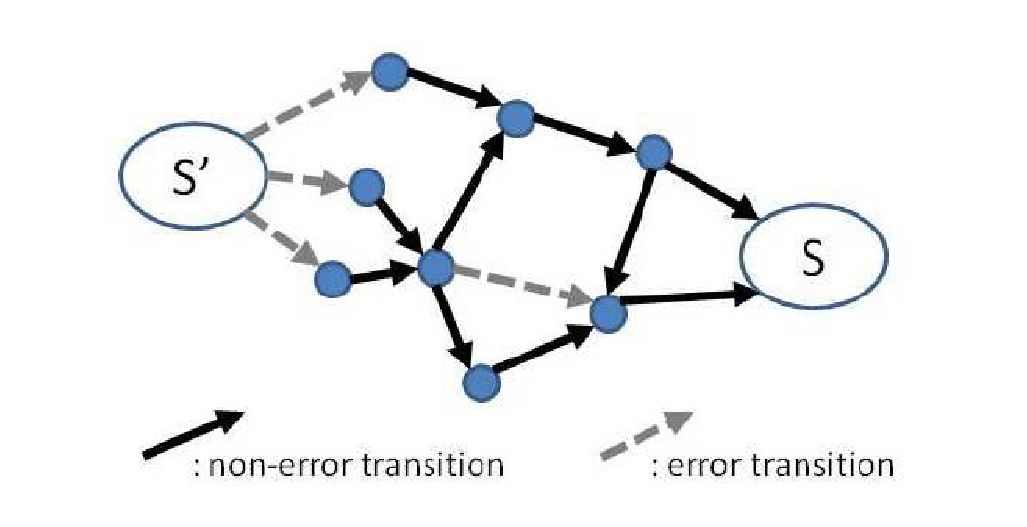
\epsfig{file=rseg.eps,width=60mm}
\caption{Illustration of the recovery operation}
\label{fig.sfrch} 
\end{center}
\end{figure}  
In this figure, the states in set $S'$ are computed  
as the precondition of states in $S$ through those transitions in the figure.  
Each path from $S'$ to $S$ is a recovery segment. 
$S$ and $S'$ may overlap.  
The blue circles represent states in the recovery segments.  
If we calculate $S'$ out of $S$, 
then, for each state $q'\in S'$, we can find a path from 
$q'\in S'$ via a path in the recovery segment to another state $q\in S$.  
The maximal number of errors in a recovery segment is 2.  
Thus the protagonist has a strategy to recover from errors in $S'$ to $S$ 
even when 2 errors happen in the corresponding recovery segment.  
When $S'=S$, then $S$ is a fixed point to the precondition 
operator through the recovery segments in the figure.  

Now we formally define the concept that we explained with Figure~\ref{fig.sfrch}.  

\begin{definition}{\bf ($k$-safety):} 
\label{k-safe}
Given a $k\in\nnneg$, 
a state $q$ is called \mbox{$k$-safe} with respect to 
a safety region $S\subseteq Q\smallsetminus F$ of non-failure states, 
denoted $q\in\safe_k(S)$, if there 
is a strategy for the protagonist to guarantee that 
we can reach back to $S$ from $q$, provided that
the overall count of errors is at most $k$.
\qed 
\end{definition}

However, the definition can be subtle in its interpretation.  
Specifically, the ability to stand against one wave of $k$ errors 
is not the same as that against repeated recovery 
from waves of $k$ errors.  
If the recovery mechanism is not designed properly, 
the system may gradually lose a bit of control after each wave of $k$ errors 
and eventually degrade to system-level failure. 

\begin{example} 
{\bf (Fault-tolerant computer architectures):}  
Consider Example~\ref{exmp.avi} with $2k+1$ processor copies, with the objective to maintain majority checks and to identify the bad processors. 
Indeed, according to the first, na\"ive solution, any safe state with a recovery strategy to $Q\smallsetminus F$ is good.   
After $k$ processor copies fail, the majority checks are still capable to maintain the correctness of the combined behavior to follow the design of the original system.
There seems to be nothing to do after $k$ errors.  
Thus, na\"ively, we can choose those states as the safety region if, at those states, majority checks still work.

However, there is no expectation that the system will be able
to recover at any point in the future into a situation where it can bear 
another wave of $k$ errors.   
It will fail and lose the function of majority checks just after one more error.  
In contrast, in this work, we aim to propose a dense error resilience criterion that 
given no more errors for enough time to allow recovery, 
the system will eventually recover to resilience to $k$ dense errors again. 
%Note that `enough time' is a system parameter that refers to the time required for recovery, provided no further errors occur.
\qed 
\end{example} 

To look at this issue in more detail, 
please consider the transition system with four states, 
including a single failure state
(state $4$, marked by a double line) shown in Figure~\ref{fig:example}.
The controlled transitions are depicted as black solid arrows, 
the error transitions are depicted as red dashed arrows.
For $S=Q\smallsetminus F=\{1,2,3\}$, all states in $S$ are in $\safe_0(S)$.
For all $k \geq 1$, we have $\safe_k(S)=\{1,2\}$:
the protagonist can simply stay in $\{1,2\}$ 
during the safety phase of the game, and once the antagonist 
plays an error transition, the game progresses 
into the recovery segment, where the protagonist's objective 
is satisfied immediately.
This outlines the difference between $k$-sfrch-ty and 
the linear time property
of being able to repeatedly tolerate waves of up to $k$ errors, 
which would only be satisfied by states $1$ and $2$ for 
$k = 1$, and only for state $1$ for $k = 2$.

\begin{figure}[t]
\begin{center}
\psset{xunit=26mm,yunit=7mm}
\begin{pspicture}(0,-.15)(3,1.4)
% \pnode(0,.6){0}
\rput(0,0){\circlenode{1}{$1$}}
\rput(1,0){\circlenode{2}{$2$}}
\rput(2,0){\circlenode{3}{$3$}}
\rput(3,0){\circlenode[doubleline=true]{4}{$4$}}
% \ncline{->}{0}{1}
\nccircle{->}{1}{.35}
\nccircle{->}{2}{.35}
\nccircle{->}{3}{.35}
\ncarc[linecolor=red,linestyle=dashed]{->}{1}{2}
\ncarc{->}{2}{1}
\ncarc[linecolor=red,linestyle=dashed]{->}{2}{3}
\ncarc{->}{3}{2}
\ncline[linecolor=red,linestyle=dashed]{->}{3}{4}
\end{pspicture}
\end{center}
\caption{\label{fig:example} An example for calculating $\safe_k$}
\end{figure}

This difference raises the question 
if the rules of our game are depriving the antagonist 
of some of the $k$ errors that she should intuitively be allowed to insert in a wave.
The answer is that this is not the case 
if we use any fixed point of $\safe_k$ as $S$.
In this case, the protagonist would regain the capability to endure a wave of $k$ errors when reaching a safe state after recovery.
Instead of depriving the antagonist, 
one could say that we reset the number of errors in any recovery 
segment that the antagonist can inject to $k$.
Thus such a fixed point of $\safe_k$ should consist of 
states, from which we can use a control mechanism to fend off 
repetitive waves of $k$ dense errors in the recovery segments.  
For convenience, we call states in such a fixed point of $\safe_k$  
the $k$-resilient states.

For a state to be in $\safe_k(S)$, 
the system (protagonist) has a strategy to recover to $S$, 
given that a long enough execution commenced 
without another round of $k$ errors happening.
We say that two successive errors are in the same 
\emph{group of dense errors} 
if the sequence of states separating them 
was not long enough for recovery to the safety region.
Vice versa, if two successive errors are far enough apart 
such that the protagonist can guarantee recovery in this separation, 
then they do not belong to the same group.

To check whether recovering to $S$ by the protagonist (the fault-tolerance mechanism)
is always possible, provided that at most $k$ errors occurred during 
a recovery segment, observe that nesting 
$\safe_k$ once, i.e., $\safe_k(\safe_k(\cdot))$, corresponds
to tolerating up to two rounds of up to $k$ dense errors, and so forth.
Thus, for $S$ to be a target of recovery for $k$-resilience, 
$S$ must be a fixed point of the operator
$\safe_k$ from Definition~\ref{k-safe}, or, equivalently, 
$S=\safe_k(S)$ must hold.  
Moreover, if $S$ is the greatest fixed point to $k$-resilience, then we we can apply 
$\safe_k()$ any number of times to $S$ and still obtain $S$.  
Computationally, the greatest fixed point of $\safe_k$ can be constructed as 
by executing  
\begin{center} 
$\safe_k(\safe_k(\safe_k(\ldots\ \safe_k(S\big)\ldots)))$,
\end{center}  
using a sufficiently deep nesting that a fixed point is reached.

Note that this fixed point $x$ to $x=\safe_k(x)$ is what we are really interested in, 
while $\safe_k(S)$ for a given $S$ is an intermediate result that does not 
guarantee survival of the systems after waves of dense errors.
If this greatest fixed point
$$R = \bigcup\{X \subseteq S \mid X = \safe_k ( X )\}$$ is non-empty, 
the protagonist's strategy for 
the fixed point (guaranteeing eventual recovery 
to a state in the fixed point within no more than $k$ errors, i.e., $k$-resilience) 
can be used to control the recovery mechanism, 
constraining its transitions to follow its winning strategy.

As explained in the introduction, there can be several natural control problems in our safety resilience game.
First, the system designers may want to know whether the chosen safety region $S$ can be supported by the recovery mechanism for resilience level $k$.  
Second, they may want to get design support for choosing the safety region for achieving resilience level $k$.  
Finally, they may want to know the maximal resilience level that they can achieve. 

we will explain the algorithm for constructing $\safe_k(\cdot)$ and evaluating $k$-resilient states.


\section{Safety resilience games}
A system is $k$-resilient if it
can be controlled to tolerate infinitely many groups of up to $k$ dense errors, 
provided that the system is given enough time to recover between these groups.
As we have explained, in systems developed with defensive mechanism against errors,  
when errors are detected, recovery procedures should be activated.  
The major challenge is to decide given a set of failure states and a safety region,
whether 
the recovery mechanism can support a resilience level required\label{reply1.prescribed.2.required} by the users. 
Our goal is to develop techniques with a solid foundation to 
assist the system designers in evaluating the resilience of their systems, 
to synthesize the controller strategy for the required resilience level, and 
to achieve the maximal resilience level. 


We now formally define the safety resilience game played between a 
system (the protagonist) and an error-injector (the antagonist).  
Initially, the two players are given a 2-player concurrent game structure $\calk$,  
a pebble in $r$,  
a set $F\subseteq Q$ of failure states, and 
a safety region $S\subseteq Q\smallsetminus F$. 
Then the recovery region consists of states in $Q\smallsetminus (F\cup S)$.  
The two players together make decisions and move the pebble from state to state.   
The antagonist tries to deflect a play into $F$ by injecting sufficiently many errors, while
% On the other hand, 
the protagonist tries to avoid that the pebble reaches $F$. 
To achieve this, the protagonist can use the recovery region as the safety buffer and try to 
get back to $S$ as soon as the play is deflected from $S$ 
to the recovery region.  
If a system is resilient to $k$ errors, then it means that 
the protagonist can handle up to $k-1$ errors while in the recovery region.  
Thus when checking whether a system is resilient to $k$ errors, 
we only need to check those recovery segments with no more than $k-1$ errors. 

In the following, we formalize the concept.  

\begin{definition} \label{def.srgs} 
{\bf (Safety resilience game structure):} 
Such a structure is a pair $\langle \calk, F\rangle$ with the following 
restrictions. 
\begin{list1} 
\item $\calk$ is a 2-player concurrent game structure 
  $\langle Q,r,P,\lambda,E_1,E_2,\delta\rangle$.  
  Conceptually, the first player represents the system / the protagonist, while 
  the second player represents the error model / the antagonist.  
\item $E_2$ is partitioned into error and and non-error moves $E_{\emerr}$ and $E_{\emnerr}$, respectively.
%   The error moves are characterized by a condition `$\emerr$', while the non-error moves  are characterized by a condition `$\emnerr$'.
We require that only the 2nd player can issue $\emerr$ moves.  
Moreover, $E_{\emnerr}$ must be non-empty. 
\item $F$ is the set of failure states in $Q$ with $r\not\in F$.   
\end{list1} 


The antagonist can choose if she wants to respond on a move of the protagonist with an error move. \label{abstraction}
We allow for different non-error moves to reflect `normal' nondeterministic behavior, e.g., caused by abstraction. 
We allow for different error moves to reflect different errors that can occur in the same step.

We sometimes refer\label{reply1.reffer} to transitions with $\emerr$ moves by the antagonist as \emph{error transitions} and 
to transitions with  $\emnerr$ moves by the antagonist as \emph{controlled transitions}.  

For a party $A \subseteq \{1,2\}$, we refer with $\overline{A} = \{1,2\} \setminus A$ to the players not in the party, and by $E_A$ to the moves made by the players in $A$, that is, $E_{\{1,2\}} = E_1 \times E_2$, $E_{\{1\}} = E_1$, etc.

% For convenience of algorithm explanation, we require that $\delta$ is 
% a total function.  
% This does not compromise the expressiveness of $\calk$ for 
% modeling undefined moves since we can create an auxiliary failure state in $F$ 
% revise $\calk$ so that all undefined moves end at this failure state. 

The antagonist can use both error and non-error moves to influence the game.
In a simple setting, the antagonist may only have the choice to insert error-moves, while there is only a single controlled transition.
In this simple case, the protagonist can choose the successor state alone unless the antagonist plays an error transition.  
% Such simple systems can be useful in simplifying the error models. 
Specifically, a safety resilience game structure is {\em simple} if $E_2$ contains only one error move.
\label{reply1.2.complexities} 
Considering simple safety resilience game structures leads to lower 
complexities, as it changes reductions from reachability in games (PTIME-complete \cite{Immerman81})
to reachability in graphs (NL-complete \cite{Papadimitriou94}).
% % the 
% % following two conditions are satisfied. 
% % \begin{list1} 
% % \item There are only two moves that the antagonist can issue, 
% %   the $\emerr$ move (representing a system error) and 
% %   the $\emnerr$ move (representing no system error). 
% % \item The destination states of error transitions are independent of   
% %   the moves selected by the protagonist.  
% %   \qed 
% % \end{list1} 
% 
% \pagebreak \pagebreak
% Thus, we require that, for every state $q$ and 
% every move vector $[e_1,e_2]$, the following constraints are true. 
% \begin{list1} 
% \item If $e_1\in\{\emerr,\emnerr\}$, then $\delta(q,e_1,e_2)=\perp$. 
% \item If $e_2\not\in\{\emerr,\emnerr\}$, then 
%     $\delta(q,e_1,e_2)=\perp$. 
% \item For every state $q\in Q\smallsetminus F$, there exists an $e\in E$ with 
%   $\delta(q,e,\emnerr)\neq \perp$.  
%   This means every functional state has a controlled successor when no 
%   error occurs.  
\qed 
% \end{list1} 
\end{definition} 

Note that, in the game structure, only one system player and one error model player 
are allowed.   
This is purely for the simplicity of algorithm presentation.  
With proper reduction techniques, we can easily convert 
a game structure with more than one system player and 
more than one error model player to the structure in Definition~\ref{def.srgs}.  
The standard technique would be using the transition rules of 
the product automata of the system players for the protagonist while 
using the transition rules of the product automata of the error model players 
for the antagonist.  
In fact, we indeed use this reduction technique in our experiment for 
analyzing the resilience levels of multi-agent systems.  

From now on, we assume that we are in the context of a 
given safety resilience game structure $\calg=\langle \calk,F\rangle$. 

\begin{definition}\label{def.rec.seg}
{\bf (Recovery segements):} 
We need to rigorously define {\em recovery segments}. 
A play prefix $\rho$ is a {\em recovery segment} to safety region $S\subseteq Q\smallsetminus F$ 
if it satisfies the following constraints. 
\begin{list1} 
\item %$\rho(0)=r$ or
      $\rho(0)\in S$. 
\item If $|\rho|=\infty$, then all states in $\rho[1,\infty)$ are 
  in $Q\smallsetminus(S\cup F)$. 
  In this case, $\rho$ is called a failed recovery segment. 
\item If $|\rho|\neq \infty$, then all states in $\rho[1,|\rho|-2]$ 
  are in $Q\smallsetminus(S\cup F)$ and 
  $\emlast(\rho)=\rho(|\rho|-1)$ is either in $F$ or $S$.    
  If $\emlast(\rho)\in F$, $\rho$ is also a failed recovery segment; 
  otherwise, it is a successful one. 
\end{list1} 
We use $\mbox{\em level}(\rho, S)$ to 
denote the number of error moves between states in $\rho$  
with respect to the safety region $S$:
$\mbox{\em level}(\rho, S) \defn \big\lvert\{i \in [0,|\rho|-1) \mid \rho_e(i) \models E_{\emerr}\}\big\rvert$.
\qed 
\end{definition} 

As stated in the introduction, we propose 
a game-theoretic foundation for resilience analysis of software systems. 
With this perspective, the protagonist acts as a maximizer, who wants to maximize the 
resilience levels along all plays.
For this, the protagonist fixes a strategy that describe what he is going to do on each play prefix.
The antagonist acts as a minimizer, who wants to minimize the resilience level.
She can resolve nondeterminism and inject errors in order to achieve this, and (although this plays no major role in this setting) she knows the strategy the protagonist has fixed and can use this knowledge in principle.

The goal of the protagonist is therefore the same as the goal of the system designer: to obtain a strategy that offers a maximal level of resilience in a safety game. 
\label{reply1.memoryless.unbounded.resilience} 
However, in order to avoid degenerate behavior where the protagonist benefits from being in the recovery phase and from the antagonist therefore being allowed less errors in the current wave of errors she may inject, we have to strengthen his obligation to eventually recover to the safe states when the environment chooses not to inject further errors.
This way, the protagonist has no incentive to cycle in the recovery region.
Consequently, he can recover to the safe region within $|Q|$ moves after the antagonist has inserted the last error of the current wave, irrespective of whether the antagonist would be allowed to insert further errors in this wave.
This is the key reason why memoryless optimal control exists for this error model, why it is reasonable to assume swift recovery, and, consequently, why it is a posteriori justified to leave the separation time between two waves implicit: the time to traverse $|Q|$ states suffices.

% this we have to be careful to define the goal rigorously 
% so that the protagonist may not choose to stay in a successful recovery segment, 
% watch the antagonist committing unboundedly many error moves, 
% and only then choose to leave the recovery segment. 
% Such degenerate scenarios are avoided in our theoretical foundation 
% since our transition function is a total function from events to 
% the destination states.  
% Thus as long as $E_2$ does not contain only the error move, then 
% there is always an non-error transition from every state.  

% Likewise, if the antagonist can deflect a play to failure, then she must be
% able to do this in $|Q|$ moves.  
% Since the antagonist is a minimizer of the resilience level in 
% the game, then, if the antagonist cannot direct a play to failure with 
% $|Q|$ errors in the recovery segment, it simply will 
% not inject any error to admit the resilience level to grow 
% unboundedly.  

Besides obtaining this from intuition, we can also consider the tree of successful recoveries for any protagonist strategy that can endure $k$ error moves by the antagonist.
The tree of recoveries from up to $k$ errors is finite according to 
the definition of successful recovery segments. 
Then for any subtree $t$ in this tree of recoveries with a node $v$ in $t$ 
such that $v$ is labeled with the same state as the root of $t$ with no error on the path,   
we can always replace $t$ with the subtree rooted at $v$.  
After the replacement, we have a tree of recoveries with no greater depth than 
the original one. 
After repeating such replacements, 
this immediately provides a translation from such a strategy with unrestricted memory 
to one with memory of size $k$ (the resilience level).
The restriction to memoryless strategies follows from the construction we give 
in Section~\ref{sec.mck}, 
which does not depend on the memory and still yields a strategy, which is memoryless.
Thus, in this work, we should define the resilience level of software systems based 
on \emph{memoryless} protagonist strategies.  

Based on the argument above, 
the gain of the protagonist in a play can be defined as follows. 

\begin{definition}
\label{def.gain} {\bf (Gain):} 
Given safety region $S \subseteq Q\smallsetminus F$, 
the gain of a play $\rho$ to $S$, in symbols $\emgain(\rho,S)$, 
denotes the maximal integer $k \in \mathbb N$ such that, 
for all recovery segments $\rho_r$ to $S$ in $\rho$, 
if $\mbox{\em level}(\rho_r,S)\leq k$, 
then $\rho_r$ is a successful recovery segment to $S$. 
\qed 
\end{definition}

The resilience level of a safety resilience game is defined 
as the maximum gain that the protagonist can guarantee in all plays 
with a memoryless strategy.  


%  
% Given a safety region $S$ and a play $\phi$ in $\calk$, 
% the gain of the protagonist in $\phi$ with respect to $S$, 
% in symbols $\emgain(\phi,S)$, 
% is defined as the maximum $k\in\nnneg$ such that 
% every recovery segment in $\psi$ with respect to $S$ 
% with no more than $k$ errors are successful. 

\begin{definition}\label{def.srgame}  
{\bf (Safety resilience game):} 
Such a game is zero-sum and defined on 
a safety resilience game structure $\calg=\langle \calk,F\rangle$ 
and a safety region $S\subseteq Q\smallsetminus F$. 
The gain of $\calg$ to $S$, in symbols $\emgain(\calg,S)$, is defined as 
the maximum gain that the protagonist can manage with memoryless strategies.  
Rigorously, 
\begin{center} 
$\emgain(\calg,S)\defn \max_{\sigma\in \Sigma^{(0)}}\min_{\sigma'\in \Sigma}
\emgain(\emplay(r,\sigma,\sigma'),S)$
\end{center} 
\label{reply1.emplay} 
Please be recall that $\emplay(r,\sigma,\sigma')$ is the play from $r$ 
according to strategies $\sigma$ and $\sigma'$ respectively of the 
two players. 
Moreover $\Sigma^{(0)}$ is the set of memoryless strategies. 

We say that the resilience level of $\calg$ to $S$ is $\emgain(\calg,S)$. 
\label{reply2.optimal}
A strategy $\omega$ for the protagonist is optimal to $S$ if 
$\min_{\sigma'\in \Sigma}
\emgain(\emplay(r,\omega,\sigma'),S)=\max_{\sigma\in \Sigma^{(0)}}\min_{\sigma'\in \Sigma}
\emgain(\emplay(r,\sigma,\sigma'),S)$.  
When $S$ is not given, 
we say that $\calg$ is {\em $k$-resilient} if there exists a non-empty $S \subseteq Q \setminus F$ with $\emgain(\calg,S)\geq k$.
\qed 
\end{definition} 

\paragraph{\bf Remark.}\hspace*{-2ex}
While the option of using memoryless strategies plays a minor role in the technical argument, it plays a paramount role in the usefulness of the resulting control strategy:
choosing memoryless strategies implies that all recovery segments are short.
In particular, all sub-paths (recovery segments) between two waves of dense errors injected by the antagonist are shorter---and usually significantly shorter---than the size of $\calg$.
In consequence, any time span long enough for traversing the recovery segment will lead to a full recovery.
It is therefore sufficient for a temporal distance we have to assume between two waves of dense errors.





\section{Alternating-time $\mu$-calculus with events}
We propose to solve our resilience game problems with an 
existing technology, i.e., model-checking of alternating-time $\mu$-calculus 
({\em AMC}) formulas.  
AMC is a propositional temporal logic 
with fixed point operators.  
For example, the following formula 
\begin{center} 
\hfill 
$\mu X.(\text{\em safe}\vee \langle 1\rangle \nxt X)$
\hfill (A) 
\end{center} 
uses least fixed point operator $\mu$ to declare a fixed point variable 
$X$ for a set of states. 
Subformula $\langle 1\rangle \nxt \phi$ existentially 
quantifies over 
the protagonist strategies that can direct the plays to a successor state 
satisfying $\phi$.  
Together, the formula specifies a set $X$ of states that can inductively reach a safe 
state with the control of the protagonist. 
Specifically, the formula says that a state is in $X$ if 
either it is {\em safe} 
or the protagonist can direct to a successor state known to be 
in $X$.  
For our game structures, we only need strategy quantification 
of up to two players.  

However, we need extend AMC with some simple syntax sugar.  
There are two extensions.  
The first is for Boolean combinations of path modalities in the 
scope of strategy quantification. 
For example, the following AMCE formula 
\begin{center} 
\hfill 
$\langle 1\rangle((\mbox{\em smoke}\Rightarrow\nxt\mbox{\em alarmOn})\vee 
\nxt\mbox{\em windowClosed})$ 
\hfill (B) 
\end{center} 
says that the protagonist can enforce either of 
the following two path properties with the same strategy. 
\begin{list1} 
\item If there is smoke, then the alarm will be turned on in the next state. 
\item The window will always be closed in the next state.  
\end{list1} 
Such a formula is not in ATL and AMC \cite{AHK02}.  

The second extension is for restricting transitions that may participate 
in the evaluation of path formulas.  
The restriction is via constraints on moves on transitions and 
can, in our extension to AMC, be specified with a  
move symbol set to the next-state modal operators.  
For example, the following AMCE formula  
\begin{center} 
\hfill $\langle 1\rangle ((\nxt^{2:\emserr}\mbox{\em alarmOn}) 
\wedge (\nxt^{\neg 2:\emserr}\neg\mbox{\em alarmOn}))$ 
\hfill (C) 
\end{center} 
says that the protagonist can 
\begin{list1}
\item turn on the alarm when an error occurs; and 
\item keep the alarm silent when no error occurs.
\end{list1} 
Before we formally present AMCE, we need define expressions for 
constraints on moves of players in transitions.  
We adapt an idea from \cite{Wang14}.  
Specifically, a {\em move expression} $\eta$ is of the following syntax. 
\begin{center} 
$\eta ::= a:e \mid \eta_1\vee\eta_2 \mid \neg \eta_1$
\end{center} 
Here, $a$ is a player index in $\{1,2\}$ and $e$ is a move symbol in $E_1\cup E_2$.  
$\vee$ and $\neg$ are standard disjunction and negation.  
% $\true$ can be seen as a shorthand of $1:E$.  
Typical shorthands of Boolean operations can also be defined out of 
$\vee$ and $\neg$.  
A total move vector can be expressed as $[e_1,e_2]$ 
where for all $a\in\{1,2\}$, $e_a\in E_a$ is the move by 
player $a$ specified in the vector.  
We say $[e_1,e_2]$ satisfies $\eta$, in symbols 
$[e_1,e_2]\models \eta$, if and only if the 
following constraints are satisfied. 
\begin{list1} 
\item $[e_1,e_2]\models a:e$ if, and only if, $e_a$ is $e$.  
\item $[e_1,e_2]\models \eta_1\vee\eta_2$ 
  if, and only if, $[e_1,e_2]\models \eta_1$ or 
  $[e_1,e_2]\models \eta_2$. 
\item $[e_1,e_2]\models \neg\eta_1$ 
  if, and only if, $[e_1,e_2]\not\models \eta_1$.   
\end{list1} 
\subsection{Syntax}
A formula $\phi$ in AMCE has the following syntax. 
\begin{center} 
$\begin{array}{rrl} 
\phi	& ::= & p 
	\mid X 
	\mid \phi_1 \vee \phi_2
	\mid \neg \phi_1 
 	\mid \mu X.\phi_1 
 	\mid \langle A\rangle \psi\\ 
\psi	& ::= &
	\mid \psi_1 \vee \psi_2
	\mid \neg \psi_1 
 	\mid \nxt^\eta \phi_1
\end{array}$ 
\end{center} 
Here, $\phi$ is a state formula, $\psi$ is a path formula,  
$p$ is an atomic proposition symbol in $P$ 
(atomic proposition set, as in Definition~\ref{def.cncgame})\label{reply1.P.x}, 
and 
$X$ is a set variable for subsets of $Q$.
The Boolean connectors are the common ones: $\vee$ for disjunction and 
$\neg$ for negation.
Note that we allow for Boolean combinations of the next operators $\nxt$ 
under strategy quantification  $\langle A\rangle$.  
This is one major difference of AMCE from AMC.  

Formula $\mu X.\phi_1$ is the usual least fixed point operation to $\phi_1$.
According to the tradition in \cite{AHK02}, 
we require that all free occurrences of $X$ in $\phi_1$ must occur
within an even number of scopes of negations.    
This is because sentences with a negative occurrence, like $\mu X. \neg X$, have no natural semantics.
A set variable $X$ is {\em bound} in a formula $\phi$ if it is inside a declaration scope of $X$.  
If it is not bound, then it is {\em free}.  
An AMCE sentence is an AMCE state formula without free set variables. 
In most cases, we are interested in specifications given as AMCE sentences.  


The $A$ in $\langle A \rangle$ is a finite set of player indices 
in $[1,2]$.
Conceptually, $\langle A \rangle\psi$ means that players in $A$ can collaborate 
to make $\psi$ true. 
For example, $\langle \{1,2\}\rangle\nxt p$ means that 
players~1 and~2 can collaborate to make $p$ true in the next state. 
We follow the notations in \cite{AHK02} and omit the parentheses in 
formulas like $\langle A\rangle \psi$.  
For example, $\langle \{2\}\rangle \nxt p$ 
and $\langle \{1,2\}\rangle \nxt p$ 
will be abbreviated as 
$\langle 2\rangle \nxt p$ and   
$\langle 1,2\rangle \nxt p$ respectively.  

We allow event 
restrictions as superscripts in $\nxt^\eta\phi_1$ 
with a move expression $\eta$.  
The operator is important in supporting the evaluation of safety resilience levels with traditional model-checking technology.  
Note that since AMC \cite{AHK02} only allows for the next-state temporal 
modality, 
only the choice of moves to the next states of a strategy matters.  
Formula $\nxt^\eta\phi_1$ is thus evaluated at states  
with respect to move vectors satisfying constraint $\eta$.  
The formula is true of a move vector $[e_1,e_2]$ if and only if 
$[e_1,e_2]\models \eta$  
implies the satisfaction of $\phi$ at state $\delta(q,e_1,e_2)$. 
Also 
$\nxt^{1:E_1}\phi_1$ can be written as $\nxt\phi_1$ in AMC \cite{AHK02} 
and 
the superscript to $\nxt$ can be omitted.    



We also adopt shorthands in the below.  
The $\beta$ refers to state or path formulas.
\begin{center} 
$\begin{array}{rcl}
\true	& \defn & p \vee \neg p \\
\false	& \defn	& \neg p \wedge p \\ 

\beta_1 \wedge \beta_2 & \defn & \neg((\neg \beta_1) \vee (\neg \beta_2)) \\ 
\beta_1 \Rightarrow \beta_2 & \defn & (\neg \beta_1) \vee \beta_2 \\

\nu X.\phi & \defn & \neg \mu X.\neg\phi \\ 

{[A]\psi} & \defn & \neg \langle A\rangle \neg\psi \\ 
\end{array}$
\end{center} 

\subsection{semantics}
In the following, we adapt the presentation style of \cite{AHK02} 
to define the semantics of AMCE inductively over the structure of the subformulas.  
The value of a state formula at a state \label{reply1.semantics.dont.understand} 
is determined by the interpretation of the set variables.  
Such an interpretation $I$ maps set variables to subsets of $Q$.  
In comparison, the value of a path formula at a state 
is determined by both the interpretation
of the set variables and the move vector chosen by the players. 
For convenience and conciseness of presentation, 
we extend the definition of interpretation of \cite{AHK02} also to 
record the chosen move vector by some players. 
Specifically, we use an auxiliary variable ``$\move$"  
for the present chosen move vector in the evaluation of path formulas. 
Given an interpretation $I$, $I(\move)$ records the chosen move vector  
of all players in $I$.  
For example, $I(\move)=[\text{\tt setAlarm},\perp]$ 
means the chosen move vector 
that player 1 sets on an alarm while player 2 does nothing under interpretation $I$. 

We need the following concept for collaborative choices of moves 
to the next states by some players. 
An {\em enforced move vector set} by $A\subseteq [1,2]$ is 
a maximal set of move vectors that agree on the choices of moves 
by players with indices in $A$. 
Specifically, given an enforced move vector set $C$ by $A$, 
we require that, for every $[e_1,e_2]\in C$,  
$[e'_1,e'_2]\in C$, and $a\in A$, $e_a=e'_a$.  
For convenience, we let $\Gamma^A$ denote the set of all 
enforced move sets by $A$.  

Following the semantics style of \cite{AHK02}, 
we can extend $I$ to be an interpretation of all state and path formulas.  
Intuitively, given a state or path formula $\beta$, 
$I(\beta)$ is the set of states that satisfy $\beta$ according to
the assumption on values of set variable values and auxiliary 
variable ``$\move$."
More precisely, 
$I(\beta)$ is a subset of $Q$ 
that satisfies the following inductive rules. 
\begin{list1} 
\item $I(p)=\{q\mid p\in \lambda(q)\}$. 
\item $I(\beta_1\vee\beta_2)=I(\beta_1)\cup I(\beta_2)$. 
\item $I(\neg\beta_1)=Q-I(\beta_1)$.

\item $I(\mu X.\phi_1)$ is the smallest set $Y\subseteq Q$ 
  with $Y=I[X\mapsto Y](\phi_1)$, where 
  $I[X\mapsto Y]$ is a new interpretation identical to $I$ 
  except that $X$ is interpreted as $Y$.

\item $I(\langle A\rangle \psi)$ is the set of states 
such that there is an enforced move vector set $C$ by $A$ such that, for all move vectors $\epsilon \in C$,  
  $I[\move\mapsto \epsilon](\psi)$ holds:
  \begin{center} 
  $I(\langle A\rangle \psi) = 
  \bigcup_{C \in\Gamma^A}
  \bigcap_{\epsilon \in C} I[\move\mapsto \epsilon](\psi)$ 
  \end{center} 
\item Given $I(\move)=[e_1,e_2]$, 
  if $[e_1,e_2]\models \eta$, then  
$I(\nxt^\eta \phi_1) = \{q \in Q \mid \delta(q,e_1,e_2) \in I(\phi_1)\}$; 
otherwise $I(\nxt^\eta \phi_1) = Q$.  

\end{list1} 
A concurrent game structure is a model of an AMCE sentence $\phi$, if its initial state $r$ is in the interpretation of $\phi$ ($r \in I(\phi)$) for any interpretation $I$.

Note that, strictly speaking, AMCE does not add much to the 
expressiveness of AMC.  
In the literature, propositions have often been used to 
record events.  
Intuitively, we would need one atomic proposition for each event to mark that it has just occurred.
This event marker would be true exactly at states right after the event happened. 
(One would possibly have to create multiple copies of states to reflect this.)
 
As discussed in \cite{Wang04}, such a modeling technique leads to an unnecessary 
blow up of the state space, which could be exponential in the number 
of players in general concurrent games.  
\label{reply1.event.blowup} 
By properly selecting 
the transitions with respect to operators like $\nxt^\eta$, 
such auxiliary propositions are not necessary when encoding the state space.  
Thus, AMCE can also be of interest to practitioners for the
efficient analysis and verification of general concurrent games.


\section{Resilience level checking algorithm}
In Subsection~\ref{subsec.ideas}, we have proposed the 
idea of the $\safe_k(\cdot)$ operator and proposed 
to use its greatest\label{reply2.empty.fixed point} fixed point 
for the evaluation of $k$-resilience.
In the following, we first establish some properties of $k$-safety 
and then use AMC model-checking technology to solve the 
safety resilience games.  
\subsection{High-level description of the algorithm}
The following lemma shows the sufficiency of $k$-safety as a building block for 
solving safety resilience games.

\begin{lemma} 
\label{fixed point}
For a safety resilience game $\calg$, 
$\safe_k(\cdot)$ has a greatest fixed point.
\end{lemma}
\pf 
The lemma follows from the facts that
the function $\safe_k$ is monotonic
($S \subseteq S'$ implies $\safe_k ( S ) \subseteq \safe_k ( S' )$ 
because a winning strategy for the protagonist 
for $S$ is also a winning strategy for $S'$ 
for all states in $\safe_k(S)$) and operates on a finite domain.
\qed


For the example in Figure~\ref{fig:example}, 
considering $S=\{1\}$ ($\{1\}=\safe_2(\{1,2,3\})$), 
the only state in $S$, state $1$, is $2$-resilient: 
it can recover with the recovery strategy to always go to the left.

The set of $k$-resilient states of $\calg$, 
can be calculated as the greatest solution to 
$S=\safe_k(S)$ with $S\subseteq Q\smallsetminus F$. 
Technically\label{reply2.technically.comma} we can start the inductive calculation of the greatest fixed point 
from base case $S_0 = Q \smallsetminus F$, 
and successively calculate $S_{i+1} = \safe_k(S_i)$, 
for each $i\geq 0$. 
The set of $k$-resilient states is then the limit $S_\infty$.  
As soon as we have $S_{i+1}=S_i$, a fixed point is reached.
We then have $S_i=S_\infty$ and can stop the 
inductive construction.  
Since $S_0$ is finite and $S_{i+1}\subseteq S_i$ holds for all $i\geq 0$, 
we will eventually reach a $j$ with $S_{j+1}=S_j=S_\infty$. 
\subsection{Realization with AMCE model-checking}
We need formally define the interaction among strategies of players. 
We borrow the notation of function composition. 
Given two partial functions $\beta_1$ and $\beta_2$, 
we use $\beta_1\circ \beta_2$ to represent their composition.  
Specifically, we have the following definition.  
\begin{center} 
$\beta_1\circ\beta_2(a)=\left\{\begin{array}{ll} 
\beta_1(a) & \mbox{ if } \beta_2(a)\mbox{ is undefined}.\\
\beta_2(a) & % \mbox{ if } \beta_1(a)\mbox{ is undefined}.  \\
% \mbox{undefined} & 
\mbox{otherwise} 
\end{array}\right.$
\label{reply1.compose} 
\end{center} 
% Note that, if $a$ is defined in both $\beta_1$ and $\beta_2$, 
% then $\beta_1\circ\beta_2(a)$ is undefined. 
% 
For our purpose, a partial strategy vector is a mapping from $\{1,2\}$ to $\Sigma$ 
and can be undefined for some players in $\{1,2\}$.  
It is for a party $A\subseteq \{1,2\}$ if it is defined only for players in $A$
and represents a collaborative strategy of the players with a 
defined strategy in $A$.  
It is total if it is defined for all players.  


For convenience, we also define partial move vectors 
as mappings\label{reply2.mapping.s} from $\{1,2\}$ to $E$.  
A partial move vector is for a party $A\subseteq\{1,2\}$ if it is defined only for players in $A$.  
It is total if it is defined for all players in $\{1,2\}$.  
Given two partial move vectors $\gamma_1$ and $\gamma_2$, \label{reply1.m2gamma} 
we define $\gamma_1\circ\gamma_2$ to represent the composition of 
the two vectors.  

Given an $S$, 
we propose to construct $\safe_k(S)$ in an induction on\label{induction.on.k} $k$.  
We need the following preliminary concepts for the presentation. 


\begin{definition} 
\textbf{(Traps)}
\label{def.traps}
For $A\subseteq \{1,2\}$,
a {\em trap} for $A$ is a subset $Q'\subseteq Q$ 
that party $\{1,2\}\smallsetminus A$ has a strategy vector $\beta$ 
to keep all plays from leaving $Q'$.  
Formally, we require that, for every $q\in Q'$ 
and partial move vector $\gamma$ for $A$, 
there exists a partial move vector $\gamma'$ for $\{1,2\}\smallsetminus A$ 
such that $\delta(q,\gamma\circ\gamma'(1),\ldots,\gamma\circ\gamma'(m))\in Q'$. 
\qed
\end{definition}

\subsubsection{Base case, sfrch0(S)}

In the base case, 
$\safe_0(S)$ characterizes those states, from which the protagonist 
can direct the plays to 
$S$\label{reply2.those.states.that.can.goto.S}   
 and 
stay there via a protagonist strategy when there is no error injected by 
the antagonist. 
Thus $\safe_0(S)$ is the greatest trap for the antagonist to $S$ when no error happens and 
the greatest solution to the following equation. 
\begin{center} 
\label{reply2.SPrime}
$X=\left\{q \left| \begin{array}{l}
	q\in X\cap S, e\in E_1, \\
	\forall e'\in E_2(e' \neq \emnerr\Rightarrow \delta(q,e,e') \in X) 
	\end{array}\right.\right\}$. 
\end{center} 
In AMCE, we can alternatively define $\safe_0(S)$ as follows. 
\begin{center} 
\label{reply2.smallX}
$\safe_0(S)\defn \nu X.(S\wedge\langle 1\rangle \nxt^{\neg 2:\emserr} X)$.  
\end{center} 
This is the usual safety kernel of $S$, which consists of those states, from 
which any controlled transition is safe.  
It can be computed by the usual greatest fixed point construction.

\begin{lemma}
\label{lem:NLSafe0}
$\safe_0(S)$ can be constructed, together with a suitable memoriless
control strategy, in time linear to the size of $\calg$.
\end{lemma}
\pf 
A state $q\in S$ can stay in $\safe_0(S)$ if there is a choice $e\in E_1$ 
such that for all $f\in E_2$, $\delta(q,e,f)\in \safe_0(S)$.  
Basically, we can use the typical approach of iterative elimination 
to calculate $\safe_0(S)$. 
That is, we first let $K_0=Q-S$.  
Then we a sequence of mutually disjoint sets 
$K_1,K_2,\ldots,K_i,\ldots$ such that 
for all $i\geq 1$, states in $K_{i+1}$ can be shown to be not 
in $\safe_0(S)$ by evidences of states in $K_i\cup \ldots\cup K_0$.    
Linear time can be achieved with careful book-keeping of the choices of 
moves at all states in $S$. 
We need a counter $c_q$ for each $q\in S$ initialized to 
$|E_1|$ for the initial number of candidate choices of moves. 
Then for each $[q,e]\in S\times E_1$, we need a Boolean flag $b_{[q,e]}$ 
initialized to $\true$ to represent that 
$\{[e,f]\mid f\in E_2\}$ is still a valid choice of moves at $q$ to 
satisfy $\safe_0(S)$. 
For each state $q$, we also need to maintain a list of transition source states. 
That is, for each $\delta(q',e,f)=q$, we need 
record $[q',e,f]$ in list $L_q$.  
Then the iterative elimination proceeds as the algorithm in 
table~\ref{tab.safe0}.  
\begin{table}[!t]
\caption{Algorithm for $\safe_0(S)$ by iterative elimination} 
\label{tab.safe0}
\procbegin \noindent 
$\safe_0(S)$  
\begin{algorithmic}[1]
\FORNLINE {$q\in S$} $c_q=|E_1|$ \ENDFORLINE 
\FORNLINE {$q\in S, e\in E_1$} $b_{[q,e]}=\true$ \ENDFORLINE 
\STATE Let $i=0$ and $K_0=Q-S$. 
\WHILE {$K_i\neq \emptyset$} 
  \STATE Let $K_{i+1}=\emptyset$. 
  \FOR {$q\in K_i$ and $[q',e,f]\in L_q$} 
    \IF {$b_{[q',e]}$ is $\true$} 
      \STATE Let $c_{q'}=c_{q'}-1$. 
      \IFNLINE {$c_{q'}$ is $0$} add $q'$ to $K_{i+1}$.  \ENDIFLINE  
    \ENDIF 
    \STATE Set $b_{[q',e]}$ to $\false$. 
  \ENDFOR
  \STATE Increment $i$ by $1$.  
\ENDWHILE 
\RETURN $S-(K_0\cup \ldots \cup K_i)$.  
\end{algorithmic}
\procend 
\end{table} 
The algorithm is linear time since each transition $\delta(q,e,f)$ is 
checked exactly once. 
\qed
\subsubsection{Inductive cases, sfrchk(S)}
Now we explain how to define the inductive cases of $\safe_k(S)$. 
The condition is for those states from which plays can be directed to 
$S$ via a recovery segment in $Q\smallsetminus (S\cup F)$ 
with $k$ or less errors injected by the antagonist. 
An intermediate step for the construction of $k$-sfrch states is the construction 
of an attractor\label{reply2.attractor} that controls, through controlled moves, 
the play prefixes to stay in a 
subset $L\subseteq Q\smallsetminus F$ of non-failure states. 
As only controlled (non-error) moves are allowed, 
this is merely a backward reachability cone.

The \emph{controlled limited attractor set} of a set $X$ for a
limited region $L\subseteq Q$, denoted $\cla_L(X)$ is the set 
from which there is a protagonist strategy to move to $X$ without leaving $L$ 
and errors injected by the antagonist.  
Technically, $\cla_L(X)$ is the least solution to 
equation:\label{reply2.cla} 
\begin{center} 
$Y = X\cup\left\{q\left| \begin{array}{l} 
q\in L,e\in E_1,\\
\forall e'\in E_2\smallsetminus \{\emerr\}( \delta(q,e,e')\in Y)
\end{array}\right.\right\}$.   
\end{center} 
The controlled limited attractor set 
$\cla_L(X)$ can be constructed using simple backward reachability 
for $X$ of controlled transitions through states of $L$.  
In AMCE, this can be constructed as follows. 
\begin{center} 
\label{reply2.cla.alg}
$\cla_L(X)\defn \mu Y. (X\vee(L\wedge \langle 1\rangle \nxt^{\neg 2:\emserr} Y))$
\end{center} 
Note that the protagonist must use the same move irrespective 
of the move of the antagonist to both stay in $L$ and approach $X$, 
provided that the antagonist does not inject an error.




The controlled limited attractor set\label{reply2.limit.attractor} 
$\cla_L(X)$ is used in the construction of $\safe_k(S)$.  
We further construct a descending chain 
$V_0 \supseteq V_1 \supseteq \ldots\supseteq V_{k-1}$ of limited attractors $V_i$. 
From $V_i$ we have an attractor strategy towards $S$ for the protagonist, 
which can tolerate 
up to $i$ further errors.
The respective $V_i$ are attractors that avoid failure states.  \label{reply2.error2failure} 
Moreover, from a state in $V_i$ with $i>1$, 
any error transition leads to $V_{i-1}$.  

A state $q\in Q$ is \emph{fragile} for a set $B\subseteq Q$ 
if, for all moves of the protagonist, at least one of its successors is outside of $B$.
(The intuition is that this is an error move, and for simple safety resilience game structures, we can restrict the definition to failure states.)
The set of fragile states for $B$ is 
\begin{center} 
$\frag(B) \defn 
\{q\mid \forall e\in E_1 \exists e'\in E_2(\delta(q,e,e')\notin B)\}$.
\end{center} 
In AMCE, we have the following formulation of $\frag(B)$.  
\begin{center} 
$\frag(B)\defn [ 1 ] \nxt \neg B$.  
\end{center} 
Technically, it is, however, easier to construct its dual
\begin{center} 
\label{reply2.easier.frag.B} 
$Q \smallsetminus \frag(B) = \langle 1 \rangle \nxt B$. 
\end{center} 
This dual can be constructed using a controlled backward reachability to $B$ with 
any strategy of the protagonist.   


The limited regions $L_i$ of states allowed when approaching 
$S$ also form a descending chain 
$L_0 \supseteq L_1 \supseteq \ldots \supseteq L_k$.
%
Using these building blocks, we can compute the $k$-sfrch states 
as follows. 
The states in $L_{i+1}$ are the non-failure states from which all 
error transitions lead to a state in $V_i$.
The sets $V_i$ contain the states from which there is a
controlled path to $S$ that progresses through $L_i$; 
all error transitions originating from any state 
of this path lead to $V_{i-1}$.
$V_0$ is therefore just the set of states from 
which there is a controlled path to $S$.

From all states in $V_{k-1}$, the protagonist 
therefore has an optimal strategy in the recovery segment  
of the game described earlier:
if the antagonist can play at most $k-1$ errors, 
then the protagonist can make sure that $S$ is reached.

Starting with $L_0 \defn Q \smallsetminus F$ that 
characterizes cones on the way to $S$ 
without any errors, 
we define the $V_k$'s and $L_k$'s inductively by
\begin{center} 
$L_k\defn L_0 \smallsetminus \frag(Q\smallsetminus \cla_{L_{k-1}}(S))$,
\end{center}

In AMCE, this can be defined inductively as follows. 
\begin{center} 
$\begin{array}{rcl} 
L_0   & \defn & \neg F \\
L_k   & \defn & L_0 \wedge \langle 1 \rangle \nxt \cla_{L_{k-1}}(S).\\
\end{array}$
\end{center} 

Finally, we choose $\safe_k(S) \defn \safe_0(S \cap L_k)$.  
In AMCE, this can be expressed as follows. 
\begin{center} 
$\safe_k(S)\defn \safe_0(S\wedge L_k)$.
\end{center}
\subsubsection{Algorithm for the set of k-resilient states}
Finding a control strategy for $k$-sfrch control within 
$\safe_k(S)$ is simple:
as long as we remain in $\safe_k(S)=\safe_0(S \cap L_k)$, 
we can choose any control move that does not leave $\safe_k(S)$.
Once $\safe_k(S)$ is left through an error transition to $V_{k-1},
V_{k-2}, ...$, 
we determine the maximal $i$ for which it holds that we are in $V_i$ 
and follow the attractor strategy of $\cla_{L_i}(S)$ towards $S$.


In summary, we present our algorithms for the set of $k$-resilient states in 
Table~\ref{tab.kres}.  
\begin{table*}
\begin{center} 
$\begin{array}{rcl} 
L_0   & \defn 
& \neg F \\
L_k   & \defn 
& \neg F \wedge \langle 1 \rangle \nxt \mu y.S\vee(L_{k-1} \wedge \langle 1 \rangle \nxt^{\emserr} y \wedge \nxt L_{k-1})\\
\safe_0(S)	& \defn 
& \nu x.(S\wedge\langle 1\rangle \nxt^{\emserr} x)\\
\safe_k(S)	& \defn 
& \safe_0(S\wedge L_k)\\
\res_k(\calg) &\defn 
& \nu S. ((Q\smallsetminus F)\wedge\safe_k(S)): \mbox{the set of $k$-resilient states}\\
\end{array}$ 
\caption{Algorithm for $k$-resilient states} 
\label{tab.kres} 
\end{center} 
\end{table*} 
In fact, we have presented two algorithms. 
\label{reply2.2alg.sec} 
The first constructs $\safe_k(S)$, which can be used for checking whether the safety region $S$ 
provided by the users is indeed a good one. 
The way to do it is to simply check whether $S$ is a solution to $\safe_k(x)=x$. 


Then our second algorithm calculates $\res_k(\calg)$ as the greatest fixed point $S$ of $\safe_k(.)$  
as the recommendation for the safety region:
$$ \res_k(\calg) = \bigcup \{S \subseteq Q \mid S = \safe_k(S) \mbox{ and } S\cup F = \emptyset\}.$$
In this way, the users do not have to calculate and provide the safety region, which would be error prone.
According to the argument and lemmas from above, 
we get the following theorem. 

\begin{theorem}
\label{theorem:main} 
$\calg$ is $k$-resilient if, and only if, $r\in \res_k(\calg)$.  
\qed 
\end{theorem}
\subsection{Complexity}
A rough complexity of our resilience level checking algorithm 
straightforwardly follows the complexity of AMC model-checking.  
Specifically, the following lemma explains the maximal resilience level that we need consider. 
\label{reply2.maximal.k}
For convenience, let $k_{\max}$ be the maximal resilience level of $\calg$.  

\begin{lemma} \label{lemma.kmax} 
$k_{\max}$ is either infinite or no greater than $|Q\smallsetminus F|$.  
\end{lemma} 
\pf 
We assume that $k_{\max}$ is greater than $|Q\smallsetminus F|$ but not infinite. 
This means that there exists a failed recovery segment $\rho$ 
with $k+1$ errors injected by the antagonist. 
Since the protagonist can only use memoryless strategies, 
there must be two position indices $i<j<|\rho|-1$ with $\rho(i)=\rho(j)$ in the recovery segment 
such that at $\rho(i)$ and $\rho(j)$, 
the protagonist makes the same move while the antagonist makes different moves. 
This implies the existence of a shorter failed recovery segment $\rho[0,i]\rho[j+1,|\rho|-1]$.  
By repeating the above argument, we can eventually identify a failed recovery segment of length 
$\leq |Q\smallsetminus F|$ that contradicts the assumption and establishes the lemma. 
\qed 

With Lemma~\ref{lemma.kmax}, we can use the complexity of AMC model-checking problem \cite{AHK02} 
to 
straightforwardly establish the $O(k_{\max} |E|)^2=O(|Q\smallsetminus F|\cdot|E|)^2$ complexity of 
$\res_k(\calg)$ when $k$ is $k_{\max}$.  
In the following, we present a more detailed analysis of the complexity of our 
resilience level checking algorithm. 
All individual steps in the construction 
(intersection, difference, predecessor, and attractor) 
are linear in the 
size of the safety resilience game, and 
there are $O(k)$ of these 
operations in the construction.  
This provides a bi-linear (linear in $k$ and $|\calg|$) 
algorithm for the construction of $\safe_k$ and 
a strategy for the protagonist.  

\begin{lemma}
\label{lem:costSafe}
A memoryless control strategy for the states in $\safe_k(S)$ can be
constructed in time linear in both $k$ and the 
size $|\calg|$ of the safety resilience game $\calg$.
\qed
\end{lemma}
% again, bi-linear --> linear





The construction of $\res_k(\calg)$ uses the repeated execution 
of $(Q\smallsetminus F)\wedge\safe_k(\cdot)$.
The execution of $\safe_k(\cdot)$ needs to be repeated 
at most $|Q\smallsetminus F|$ times until a fixed point is reached, 
and each execution requires at most $O(k\cdot|\calg|)$ 
steps by Lemma~\ref{lem:costSafe}.

For the control strategy of the protagonist, 
we can simply use the control strategy from $\safe_k(S_\infty)$ 
from the fixed point $S_\infty$.
This control strategy is memoryless (cf.\ Lemma~\ref{lem:costSafe}).
\begin{lemma}
\label{lem:costRes}
$\res_k(\calg)$ and a memoryless $k$-resilient control strategy 
for $\res_k(\calg)$ can be constructed 
in $O(k\cdot |Q\smallsetminus F| \cdot |\calg|)$ time.
\qed
\end{lemma}


Finding the resilience level $k_{\max}$ for the initial state $r$
requires at most $O(\log k_{\max})$ many constructions of $\res_i(\calg)$.
We start with $i=1$, double the parameter until $k_{\max}$ 
is exceeded, and then use logarithmic search to find $k_{\max}$.

\begin{corollary}
For the initial state $r$, we can determine the resilience level 
$k_{\max} =
\max\{i\in \nnneg \mid r \in \res_i(Q \smallsetminus F)\}$ of $r$,
$\res_{k_{\max}}(Q \smallsetminus F)$, 
and a memoryless $k_{\max}$-resilient control
strategy for $\res_{k_{\max}}(Q\smallsetminus F)$ in 
$O(|Q\smallsetminus F| \cdot |\calg|\cdot k_{\max} \log k_{\max})$ time.
\qed
\end{corollary}

% Removed the following sentence: what is -\infty???
%Note that, for $\iota\notin\res_0(S\smallsetminus F)=\safe_0(S\smallsetminus F)$, $k_{\max}=-\infty$.



\paragraph{Simple safety resilience game structures.}
For simple  safety resilience game structures, checing if a state is in $\safe_0(S)$ is NL-complete\label{reply1.NL.complete}.
\begin{lemma}
\label{lem:oldNLSafe0}
Testing if a state is in $\safe_0(S)$ is NL-complete.
\end{lemma}

\begin{proof}
NL completeness can be shown by reduction to and from the repeated ST-reachability \cite{Papadimitriou94} (the question whether there is a path from a state S to a state T and from T to itself in a directed graph).
\end{proof}

Likewise, the controlled limited attractor set 
$\cla_L(S)$ can be constructed using simple backwards reachability 
for $G$ of controlled transition through states of $L$.
For 
$A = \cla_L(S)$, determining whether a state is in $A$ 
is NL-complete (see \cite{Papadimitriou94}).

The complexity of determining whether or not a state $q$ is 
in $\safe_k(S)$ thus depends on whether or not we consider $k$ 
to be a fixed parameter.
Considering $k$ to be bounded (or fixed) is natural in our context, 
because $k$ is bounded by the redundancy.

\begin{lemma}
\label{lem:NLSafek}
For a fixed parameter $k$, testing if a state $s$ of a simple safety resilience game structures
 is in $\safe_k(S)$ is NL-complete.
\end{lemma}

\begin{proof}
Testing if a state is in $L_0$ is in NL.
%
By an inductive argument, we can show that
\begin{itemize}
\item provided that testing if a state is in $L_i$ is in NL,
we can test if a state is in $A_i = \cla_{L_i}(S)$ by using the nondeterministic power to guess a path towards $S$, while verifying that we are in $L_i$ in every state we pass before $S$ is reached; and
\item if we can check if a state is in $A_i$ in NL, then we can check if it is in $Q\smallsetminus A_i$ \cite{Immerman88}, in $\frag(Q\smallsetminus A_i)$ (with one nondeterministic transition), and in $L_{i+1}=L_0 \smallsetminus \frag(S\smallsetminus A_i)$ \cite{Immerman88} in NL.
\end{itemize}

Testing that a state is in $S \cap L_k$ is therefore in NL and testing if it is in $\safe_0(S \cap L_k)$ reduces to guessing a state $t$ in $\safe_k(G)$ and an ST path (a path from $s$ to $t$ followed by a loop from $t$ to $t$), verifying for all states on the path that they are in $S \cap L_k$.

For hardness, note that the last step of the construction alone is NL-complete (Lemma~\ref{lem:NLSafe0}).
\end{proof}

If $k$ is considered an input, then reachability in AND-OR graphs can easily be encoded in LOGSPACE:
It suffices to use the nodes of an AND-OR graph as the states, the outgoing edges of OR nodes as the result of the choice of the protagonist only (while the move of the antagonist has no influence on the outcome, no matter whether or not she induces an error), and to model the AND nodes as a state, where the no-error move of the antagonist will lead in cycling in the state, while the antagonist can choose the successor from the graph when inducing an error.
Choosing $k$ to be the number of nodes of the AND-OR graph and $F$ to be the target nodes of the AND-OR graph, the target nodes of the AND-OR graph are not reachable from a state $s$ iff $s \in \safe_k(Q\smallsetminus F)$.

Given that reachability in AND-OR graphs is PTIME-complete \cite{Immerman81}, this provides:

\begin{lemma}
\label{lem:ptc}
If $k$ is considered an input parameter, then testing if a state $s$ of a simple safety resilience game structures
 is in $\safe_k(S)$ is PTIME-complete.
\qed
\end{lemma}


The complexity of $\res_k(S)$ is (almost) independent of the parameter $k$:

\begin{theorem}
The problem of checking whether or not a state $s$ is $k$-resilient for a set $S$ is PTIME-complete for all $k>0$ and NL-complete for $k=0$.
\end{theorem}

\begin{proof}
We have shown inclusion in PTIME in Lemma~\ref{lem:costRes}.
For hardness in the $k>0$ case, we can use the same reduction from the reachability problem in AND-OR graphs as for $\safe_k(S)$.

For $k=0$, $\safe_0(G)=\safe_0\big(\safe_0(G)\big)$ implies $\res_0(G)=\safe_0(G)$.
The problem of checking if a state is in $\res_0(G)$ is therefore NL-complete by Lemma \ref{lem:oldNLSafe0}.
\end{proof}

\paragraph{Hardness for general safety resilience game structures.}
For general resilience game structures, we can again use a LOGSPACE reduction from the reachability in AND-OR graphs:
We again use the nodes of an AND-OR graph as the states, and the outgoing edges of OR nodes are selected based on the choice of protagonist only.
For the AND nodes, we leave the choice to the antagonist only, whithout the need to invoke an error.
(That is, errors play no role in this reduction.
The antagonist may be allowed to insert one, but she can always obtain the same transition without doing so.)

Marking $F$ as the target nodes, we get $\res_k(Q \smallsetminus F) = \safe_l(Q \smallsetminus F)$ for all non-negative integers $k,l$, and $s \in \safe_0(Q \smallsetminus F)$ iff the target nodes of the AND-OR graph are not reachable from $s$.
With Lemmas~\ref{lem:costSafe} and~\ref{lem:costRes}, we get the following theorem.

\begin{theorem}
For all $k \geq 0$, the problems of checking whether or not a state $s$ is in $\res_k(Q \smallsetminus F)$ and $\res_k(Q \smallsetminus F)$, respectively, are PTIME-complete for general safety resilience game structures.
\end{theorem}

\chapter{Implementation Experiment}
\section{BSIL and TCL}
\subsection{Implementation} 

We implemented semi-symbolic model-checkers of BSIL and TCL with {\bf REDLIB} 
\cite{Wang03,Wang08a,Wang08b,Wang13,Wang14}
which is a free library for symbolic model-checking based on decision diagrams. 
{\bf REDLIB} supports symbolic pre-condition and post-condition calculation of discrete transitions.  
Our model-checker starts from a symbolic representataion of the initial condition. 
Then it repeatedly applies the post-condition procedure of {\bf REDLIB} to explore the symbolic state representations in the computation tree.
Our model-checker use the result in section~\ref{sec.mck.psp} to bound the exploration depth of tree.   

\subsection{Benchmarks and their experiment report} 

Then we experimented with two parameterized benchmarks.  
The first is the prisoners' dilemma described in Example~\ref{exmp.pd} with the number of prisoners as a parameter.
Then we applied the model-checker to check whether the model satisfies formula (A) and (B) in the introduction.
The time and memory usage of the model-checker is reported in Table~\ref{tab.exp.pd}.
\begin{table*}[!th]
\caption{Experiment data for the prisoners' dilemma model}
\label{tab.exp.pd}
\begin{center}
\begin{tabular}{c||c|c||c|c} \hline
\multirow{2}{*}{\#prisoners}  &\multicolumn{2}{c||}{Formula (A)} & \multicolumn{2}{c}{Formula (B)}\\ \cline{2-5}
& Time & Mem  & Time & Mem\\ \hline
2 &0.50s &72M   &0.51s &71M \\
3 &0.92s &75M   &0.88s &75M \\
4 &1.23s &83M   &1.14s &80M \\
5 &3.19s &146M  &2.90s &140M \\
6 &6.71s &388M  &6.52s &361M \\
7 &25.10s&1043M &23.11s&979M \\ \hline
\end{tabular}
\hspace*{10mm}
\parbox{50mm}{
s: seconds (computation time); \\
M: megabytes (memory usage); \\[2mm]
The experiment is conducted on a PC with Intel i7-2600k 3.4GHZ CPU 
and 8G RAM running Ubuntu 12.04. 
}
\end{center}
\end{table*}

The second benchmark is for campaign strategies 
of 2 political parties, Party $1$ and Party $2$, for seats in 
the congress.  
There are several parameters in our model, 
the number of seats in the congress, 
the amount of budget of each party in a round, 
and the number of candidates of each party in a round. 
The game is played by the chiefs of the parties, 
Chief $1$ (a gentleman) and Chief $2$ (a lady), 
who decide the amount of support that 
a candidate receive in a round.   
Candidates with more budget in a round will be elected in the round. 
If two or more candidates get the same amount of support, 
the winner will be decided randomly.  

In our model, in each round, chief 1 first decides his budget allotment, 
then chief 2 decides her budget allotment, and 
then the election result is determined.  
For example, with 3 dollars in his budget for two candidates, 
the strategy of a Chief can be written as 
$(x,y)\in\{(3,0), (2,1),(1,2),(0,3)\}$ where $x$ and $y$ 
respectively denote the support (in dollars) 
allotted to the first and the second candidates in his party. 
If Chief $1$ uses strategy $(2,1)$ and 
Chief $2$ uses strategy $(0,2)$ (Assume she has less budget.), 
the result of the round is 
that the two parties both win one seat in the round. 
On the other hand, if Chief $2$ chooses strategy $(1,1)$ instead, 
then there is no strategy for Chief $1$ to win more seats for his party. 

We use the following propositions and predicates to write 
specifications.  
For each $i\in[1,2]$ and $j\in[1,c]$ where $c$ is the number of 
candidates, 
$\textsl{elected}_{i,j}$ means the $j$'th candidate of party $i$ is 
elected now. 
Then we can use propositions $\textsl{elected}_{i,j}$ to construct 
a predicate $\textsl{win}_i$ that means party $i$ wins more seats than party $2-i$ in the round. 
Assume that the first candidate in each party is the chief. 
Then the following BSIL formula specifies that 
Chief $1$ has a strategy to make sure candidate 1 to be elected  
and in the same time allow the opponent party to win more seats in every round.
\begin{center} 
\hfill 
$\langle 1\rangle((\langle +\rangle\pevt \textsl{elected}_{1,1})
\wedge(\langle+2\rangle\pfrr \textsl{win}_2))$
\hfill (N) 
\end{center} 
Similarly, the following formula specifies that 
the chief of party 1 has a strategy to assure that his party 
can win more seats than his opponent party while allowing party two to assure 
the winning of a candidate.  
\begin{center} 
\hfill $\langle 1\rangle((\langle +\rangle \pevt \textsl{win}_1)
\wedge(\langle +2\rangle\pevt \textsl{elected}_{2,1}))$
\hfill (O)
\end{center} 
With different values of budget and candidate count, we may use our model-checker 
to analyze the strategy for achieving various goals.  
The time and memory usage data for checking formula (N) and (O) 
is in Table~\ref{tab.exp.vote}.
\begin{table*}[!th]
\caption{Experiment Data Election}
\label{tab.exp.vote}
\begin{center}
\begin{tabular}{c|c|c|c|c||c|c|c||c|c|c} \hline
\multicolumn{5}{c||}{Parameters}
&\multicolumn{3}{c||}{Formula (N)} 
& \multicolumn{3}{c}{Formula (O)}\\ \hline
$c_1$ & $b_1$ & $c_2$ & $b_2$ & $s$ & Result & Time & Mem & Result & Time & Mem\\ \hline
2&2 &2 &4 &1 &UNSAT &0.52s &61M  &UNSAT &0.53s &61M \\
2&4 &2 &4 &2 &UNSAT &1.20s &75M  &UNSAT &1.15s &75M \\
2&4 &2 &4 &3 &SAT   &0.73s &75M  &UNSAT &1.14s &75M \\
3&6 &3 &6 &3 &SAT   &1.51s &211M &UNSAT &0.93s &211M \\
3&9 &3 &6 &3 &UNSAT &9.14s &837M &SAT   &5.22s &681M \\
3&6 &3 &9 &3 &SAT   &8.74s &502M &UNSAT &8.49s &502M \\
3&9 &3 &9 &4 &SAT   &158s  &6631M&UNSAT &93.17s&5082M \\ \hline
\end{tabular}
\hspace*{2mm}
\parbox{75mm}{
$c_1$: \# candidates of party 1\\
$b_1$: total budget in a round of party 1\\
$c_1$: \# candidates of party 2\\
$b_1$: total budget in a round of party 2\\
$s$: \# of seats in the congress\\
}
\parbox{75mm}{
s: seconds (computation time)\\
M: megabytes (memory usage) \\[2mm]
The experiment is conducted on a PC with Intel i7-2600k 3.4GHZ CPU 
and 8G RAM running Ubuntu 12.04. 
}
\end{center}
\end{table*}

The experiment shows that some possibilities of using our tool to flexibly support the analysis and synthesis of collaborating strategies among several agents. 
In the experiment with the prisoners' dilemma, the prisoners are modelled as individual agents.  
In the experiment with the election game, the chairpersons of the parties are modelled as individual agents and their candidates and respective allocated budgets are modelled as numbers.  
It would be interesting to see how we can explore the techniques in modelling and specifying concurrent games with our tool.



As in the case of BSIL, we use the parametrised models of the iterated prisoners' dilemma 
as our benchmarks to check the performance of our implementation on TCL model checker.  
We use seven benchmark formulas on these models in our experiments.  
The first five benchmarks are taken from the examples (I) through (M) from the introduction.
Benchmarks (P) and (Q) are the following two properties, taken from \cite{WHY11}. 
\begin{list1} 
\item Property (P) specifies that all prisoners except Prisoner 1 can collaborate 
  to release Prisoner 1 and let Prisoner 1 decide their fate.

  $\langle 2,\ldots,m\rangle \big((\langle + \rangle \pevt \neg \mbox{\tt jail}_1) \wedge
  \bigwedge_{i \in \{2,\ldots m\}} (\langle +1 \rangle \pevt \neg \mbox{\tt jail}_i) \wedge
  (\langle +1 \rangle \pfrr \mbox{\tt jail}_i\big)$
  \hfill (P) 
\item Property (Q) specifies that Prisoner 1 has a strategy to put all other prisoners in jail while leaving her fate to them.

    $\langle 1\rangle \big( (\bigwedge_{i \in \{2,\ldots m\}} \langle + \rangle \pfrr \mbox{\tt jail}_i) \wedge
    (\langle 2,\ldots,m\rangle \pevt \neg \mbox{\tt jail}_1) \wedge \langle 2,\ldots,m\rangle \pfrr \mbox{\tt jail}_1 \big)$
  \hfill (Q) 
\end{list1} 
\begin{table*} 
\caption{Performance data of model-checking the TCL fragment}
\label{tab.perf}
\begin{center} 
\begin{tabular}{c||c|c|c|c|c|c|c|c|c} 
\hline 
\backslashbox{properties}{$m$}
& 2 & 3 & 4 & 5 & 6 & 7 & 8 & 9 & 10 \\ \hline \hline 
(I) 	
& 0.71s & 0.94s & 5.41s & 66.3s & 945s 	& \multicolumn{4}{c}{>1000s}\\ \cline{2-6} 
& 163M	& 165M 	& 185M 	& 350M	& 1307M	\\\hline 
(J) 
& 0.50s	& 0.52s	& 0.61s	& 0.71s & 1.11s	& 1.62s	& 5.77s & 20.9s	& 68.1s \\
  \cline{2-10} 
& 163M 	& 163M 	& 164M 	& 165M	& 168M	& 176M	& 214M	& 270M	& 376M	\\ \hline 
(K) 
& 0.51s	& 0.51s	& 0.6s	& 0.82s	& 1.01s	& 1.81s	& 5.54s	& 18.2s	& 48.3s	\\\cline{2-10} 
& 163M	& 163M	& 164M 	& 165M	& 168M	& 176M	& 200M	& 241M	& 318M	\\\hline 
(L) 
& 0.5s	& 0.51s	& 0.57s	& 0.74s	& 1.01s	& 1.79s	& 7.41s	& 33.8s	& 141s \\ \cline{2-10} 
& 163M	& 163M	& 164M	& 165M	& 168M	& 175M	& 232M	& 312M	& 430M \\\hline 
(M) 
& 0.51s	& 0.66s	& 19.1s & \multicolumn{6}{c}{>1000s} \\\cline{2-4} 
& 163M	& 164M	& 194M	\\\hline 
(P) 
& 0.51s	& 0.53s	& 0.61s	& 0.71s	& 1.01s	& 1.70s	& 5.38s	& 15.2s	& 53.7s	\\\cline{2-10} 
& 163M	& 163M	& 163M	& 165M 	& 168M	& 175M	& 202M	& 243M	& 295M	 \\\hline 
(Q) 
& 0.52s	& 0.52s	& 0.65s	& 0.72s	& 1.03s	& 1.85s	& 4.86s	& 16.1s	& 93.5s	 \\\cline{2-10} 
& 163M	& 163M	& 164M	& 165M	& 169M	& 177M	& 189M	& 208M	& 235M \\\hline 
\end{tabular} \\
s: seconds; 
M: megabytes. \\ 
The models are with 1 policeman and $m$ prisoners.
The experiment was carried out on an Intel i5 2.4G notebook 
with 2 cores and 4G memory, running ubuntu Linux version 11.10.  
\end{center} 
\end{table*} 
For these benchmarks, we have collected the performance data for various parameter values in Table~\ref{tab.perf}. 
For small models, the memory usage is dominated by the normal overhead, such as the representation of variable tables, state-transition tables, formula structures, etc. 
The data shows that our prototype can handle the various benchmarks, and scales well on five of the seven benchmarks.
Ignoring the overhead, it also shows the exponential growth.
The models, however, are growing exponentially, too.
We assume that this growth i the main cause of the exponential growth of the response time.

\section{Resilience}

\section{Tool implementation}
In the following, we report our implementation and experiment about checking a system's resilience to dense errors. 

We adopt {\em CEFSM} ({\em communicating extended finite-state machine})~\cite{BH89} as a convenient language for the description of abstract models of our concurrent game structures. 
A CEFSM consists of several finite-state machines extended with shared variables for the modeling of shared memory and with synchronizations for the modeling of message-passing in distributed systems.
This is justifiable since the fault-tolerant algorithms may themselves be subject to  
restrictions in concurrent or distributed computation.
Indeed, we found CEFSM very expressive in modeling the 
benchmarks from the literature \cite{CL99,RSB90}.  
\smallskip

The translation from our CEFSMs to state transition systems, 
such as finite Kripke structures, is standard in the literature. 
All state spaces, conditions, preconditions, post-conditions, 
fixed points, etc., are represented as logic formulas. 
The logic formulas are then implemented with multi-value decision diagrams 
(MDD) \cite{MD98}.  

We then took advantage of the support of REDLIB for writing down 
template automatas for constructing complex models. 
We specified a template automata with REDLIB to describe the moves of the players. 
Conceptually, the player automatas are constructed as an instance of the template automata. 
Then the whole game structure is constructed as the product of all player automatas. 
Finally, we use the API of REDLIB to do on-th-fly construction of the game structure which 
can be advantageous since unreachable states will never be generated.  

\subsection{Benchmarks and their experiment report}
We use the following five parameterized benchmarks to check the performance of our techniques. 
Each benchmark has parameters for the number of participating modules in the model.  
Such parameterized models come in handy for the evaluation of the scalability of our techniques with respect to concurrency and model sizes.  
\begin{itemize} 
\item[1.] We use the example of a fault-tolerant computer architecture 
  (Example~\ref{exmp.avi}) as our first benchmark.  
  An important feature of this benchmark is that there is an 
  assumed mechanism for detecting errors of the modules.  
  Once an error is detected, a processor can be assigned to recover the 
  module, albeit to the cost of a reduced redundancy in the executions.
\item[2.]
	Voting is a common technique for fault tolerance through 
  replication when there is no mechanism to detect errors of the 
  modules \cite{Pradhan96}.  
  In its simplest form, a system can guarantee correctness, provided less than half of its modules are faulty.   
  This benchmark implements this simple voting mechanism.  
  Every time a voting is requested, the modules submit their ballots individually.  
  Then we check how many module failures the system can endure and recover. 
\item[3.] This is a simplified version of the previous voting benchmark, where we assume that there is a blackboard 
  for the client to check the voting result.  
\item[4.] {\em Practical Byzantine fault-tolerance} ({\em PBFT}) algorithm: 
  We use an abstract model of the famous algorithm by 
  Castro and Liskov \cite{CL99}. 
  It does not assume the availability of an error-detection 
  mechanism but uses 
  voting techniques to guarantee the correctness of 
  computations when less than one third of the voters are faulty.  
  This algorithm has impact on the design of many protocols 
  \cite{AGGRW05,CMLRS06,KADCW09,GKVQ10,CWADM09} and is used in 
  Bitcoin \cite{bitcoin}, a peer-to-peer digital currency system.  
\item[5.] {\em Fault-tolerant clock synchronization algorithm}: 
  Clock synchronization is a central issue in distributed computing. 
  In \cite{RSB90}, 
  Ramanathan, Shin, and Butler presented 
  several fault-tolerance clock synchronization algorithms 
  in the presence of Byzantine faults with high probability.  
  We use a nondeterministic abstract model of the convergence averaging 
  algorithm from their paper.  
  The algorithm is proven correct when no more than one third of the 
  local clocks can drift to eight time units from the median of all clock 
  readings.  
\end{itemize}

\subsection{Modelling of the fault-tolerant systems}
Appropriate modelling of the benchmarks is always important for 
the efficient verification of real-world target systems. 
Many unnecessary details can burden the verification algorithm 
and blow up the computation, 
while sketchy models can then give too many false alarms 
and miss correct benchmarks.  
We have found that there is an interesting aspect 
in the modelling of the above benchmarks.  
Replication and voting are commonly adopted techniques for 
achieving fault-tolerance and resilience.  
Such fault-tolerant algorithms usually consist of 
several identical modules that use the same behavior templates.  
This observation implies that the identity of individual modules 
can be unimportant for some benchmarks.  
For such benchmarks, we can use counter abstraction 
\cite{ET99,Lubachevsky84} in their models.  
Specifically, with counter abstraction, 
we can model all system players with one player that keeps a counter $c(l)$ 
for each control location $l$ in the template automatas. 
Then at a state of the whole game graph, 
$c(l)$ records the number of system players at location $l$.  
With this technique, a system with $m-1$ system player and one error model player is 
then reduced to two players: one counter-abstraction player for all the system players and one 
remaining error model player. 
If a system player enters a location $l$ in a global transition, 
then in the model, $c(l)$ is incremented by one in the abstract global transition. 
If a system player leaves $l$ in the global transition, 
then $c(l)$ is decremented by one in the abstract global transition.  
But the succession of location movements of a particular player is omitted from the abstraction. 
 

We found that we can use counter abstraction to 
prove the correctness of benchmarks 1, 2, and 3. 
In contrast, the PBFT and the clock synchronization algorithms use 
counters for each module to model the responses received 
from its peer modules. 
As a result, we decided not to use counter abstraction to model 
these two algorithms in this work. 

In the following, we explain how to apply our techniques to analyze 
the resilience levels of the avionic systems 
in Example~\ref{exmp.avi}.  
The application is achieved in three steps.
We first model the system under analysis either as a plain CEFSM or with counter abstraction (if our analysis tool cannot handle the complexity of the plain CEFSM).
We then build the product automaton of the CEFSM as the resilience 
game structure except for the move vectors.  
Finally, we convert the labels on the transitions of the product automaton to 
move vectors of the two players. 
Note that the moves may not correspond to the transition labels of the CEFSM.  

\subsection*{Step 1: the construction of the CEFSM}
We first present the CEFSM model template 
of Example~\ref{exmp.avi} in Figure~\ref{fig.pm}. 
\begin{figure*}[t] 
\begin{center} 
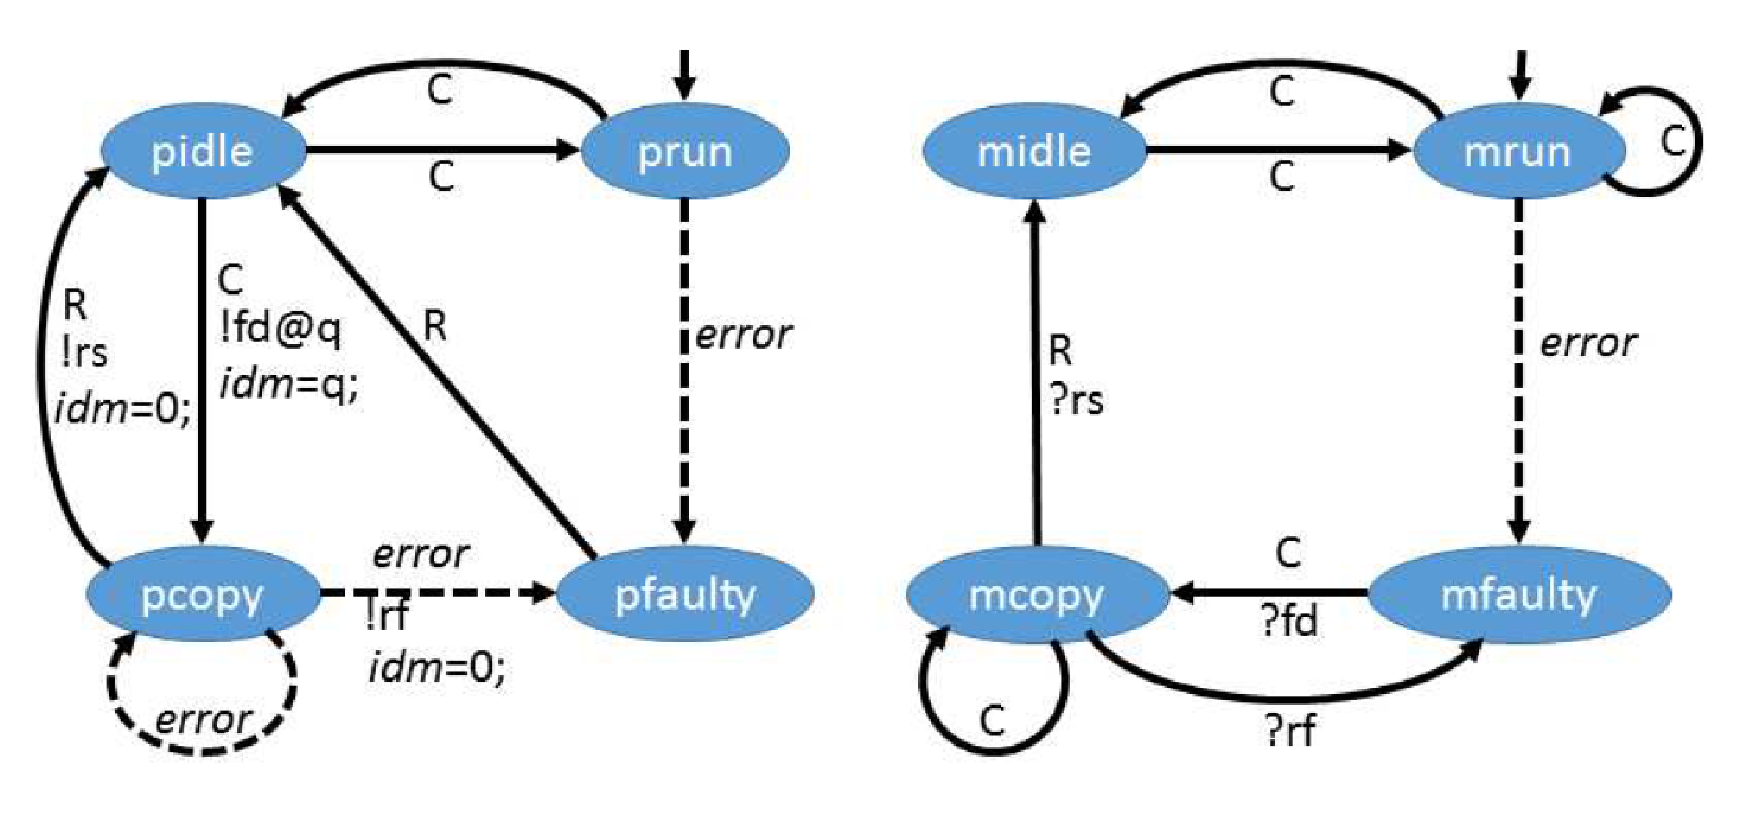
\epsfig{file=avi.eps,width=140mm} 
\caption{CEFSM templates of $n$ processors and $m$ memory copies}
\label{fig.pm}
\end{center} 
\end{figure*}
The CEFSM model has $n$ processors and $m$ memory modules. 
Figures~\ref{fig.pm}(a) and (b) are 
for the abstraction of processors and memory copies, respectively.  
The ovals represent local states of a processor or a 
memory module, while the arrows represent transitions. 
The transitions of a CEFSM are labeled with `$\emerr$', 
`C' (for Control), or `R' (for recovery).  

We also use synchronizers to bind process transitions. 
For example, when a memory module moves into a faulty state, 
an idle processor may issue an {\tt fd} (error-detected) event
and try to repair the module by copying memory contents from 
normal memory modules.  
Such error-detection is usually achieved with standard hardware.  
Note that the benchmarks are models that reflect the 
recovery mechanism, abstracting away the details of the original systems.  
A central issue in the design of this recovery mechanism is then 
the resilience level of the controlled systems.  
We need three synchronizers: 
\textit{fd} for error detection by a processor, 
\textit{rs} for recovery success, 
and \textit{rf} for recovery failure.  
The three synchronizers are used to bind a transition from a processor 
and another from a memory module into a synchronized transition.  
For example, a processor at state \textit{pidle} and 
a memory module at state 
\textit{mfaulty} may simultaneously enter their 
\textit{pcopy} and \textit{mcopy} states respectively
through synchronizers $!$\textit{fd} (for sending the synchronizer) 
and $?$\textit{fd} (for receiving). 
We also conveniently use a variable $q$ in this synchronized 
transition to capture the identifier of the memory module receiving 
the synchronizer.  
A transition without synchronization labels is considered a trivial 
synchronized transition.  
The transition system of the CEFSM operates with interleaving semantics 
at the abstraction level of the synchronized transitions. 

For counter abstraction, we need four global variables \textit{crp}, \textit{cfp}, 
\textit{crm}, and \textit{cfm} respectively 
to keep track of the numbers of running processors, faulty processors, 
running memory modules, and faulty memory modules. 
We also need a local variable \textit{idm} for each processor to record 
the faulty memory module identifier that the processor is 
responsible for recovery. 
We label the controllable, error, and recovery 
transitions respectively with `C', `$\emerr$', and `R'. 
We also label each transition with synchronizers and actions.  
At any moment, the processors and the memory modules 
may enter their running states, execute a task, and generate 
the outcome. 
A processor starts its execution from state \textit{prun} while 
a memory module starts from state \textit{mrun}. 


\subsection*{Step 2: building the product automata}
The product automata is a Kripke structure whose 
states are of is a vector $[p_1,\ldots,p_n,i_1,\ldots,i_n,s_1,\ldots,s_m]$ 
of $2n+m$ elements.  
For all $k$, $p_k$ and $i_k$ respectively represent the 
current location and the current \textit{idm} value of processor $k$ while 
$s_k$ represents the current location of memory module $k$.  
Then interleaving semantics that each time only a global transition 
(a single local process transition without synchronizers 
or two local process transition bound by a synchronizer) is executed 
is adopted to determine the transition relation from one state to another. 
Such techniques are standard in model construction.  
REDLIB can help in this regard by constructing the Kripke structure in 
an on-the-fly style to avoid the construction of those states not reachable 
from the initial state. 

\subsection*{Step 3: the labeling of the move vectors} 
After the second step, we have the game structure ready except for the 
move vectors on the transitions. 
We use $E_1=\{C,R,\mbox{\em nop}\}$, where {\em nop} represents ``no operation,"
and $E_2=\{\emnerr,\emerr\}$.  
Then we use the following three rules to label move vectors. 
\begin{list1} 
\item Every global transition with one component local process transition labeled 
	with $\emerr$ is labed with move vector $[\mbox{\em nop},\emerr\}$.  
\item Every global transition with a component local process transition labeled 
	with $R$ 	
	is labeled with move vector $[R,\emnerr]$.  
\item All other global transitions are labeled with move vector $[C,\emnerr]$.  
\end{list1} 


\subsection*{Counter abstraction of the example} 
We also use the CEFSM in figure~\ref{fig.pm} to explain counter abstraction. 
We need eight counter variables: 
{\em pr}, 
{\em pi}, 
{\em pc}, 
{\em pf}, 
{\em mr}, 
{\em mi}, 
{\em mc}, and 
{\em mf} to respectively record the 
number of processes in location prun, pidle, pcopy, pfaulty, mrun, midle, mcopy, and mfaulty
in a state.  
Then the counter abstraction of the CEFSM is in Figure~\ref{fig.pmC}.  
\begin{figure*}[t] 
\begin{center} 
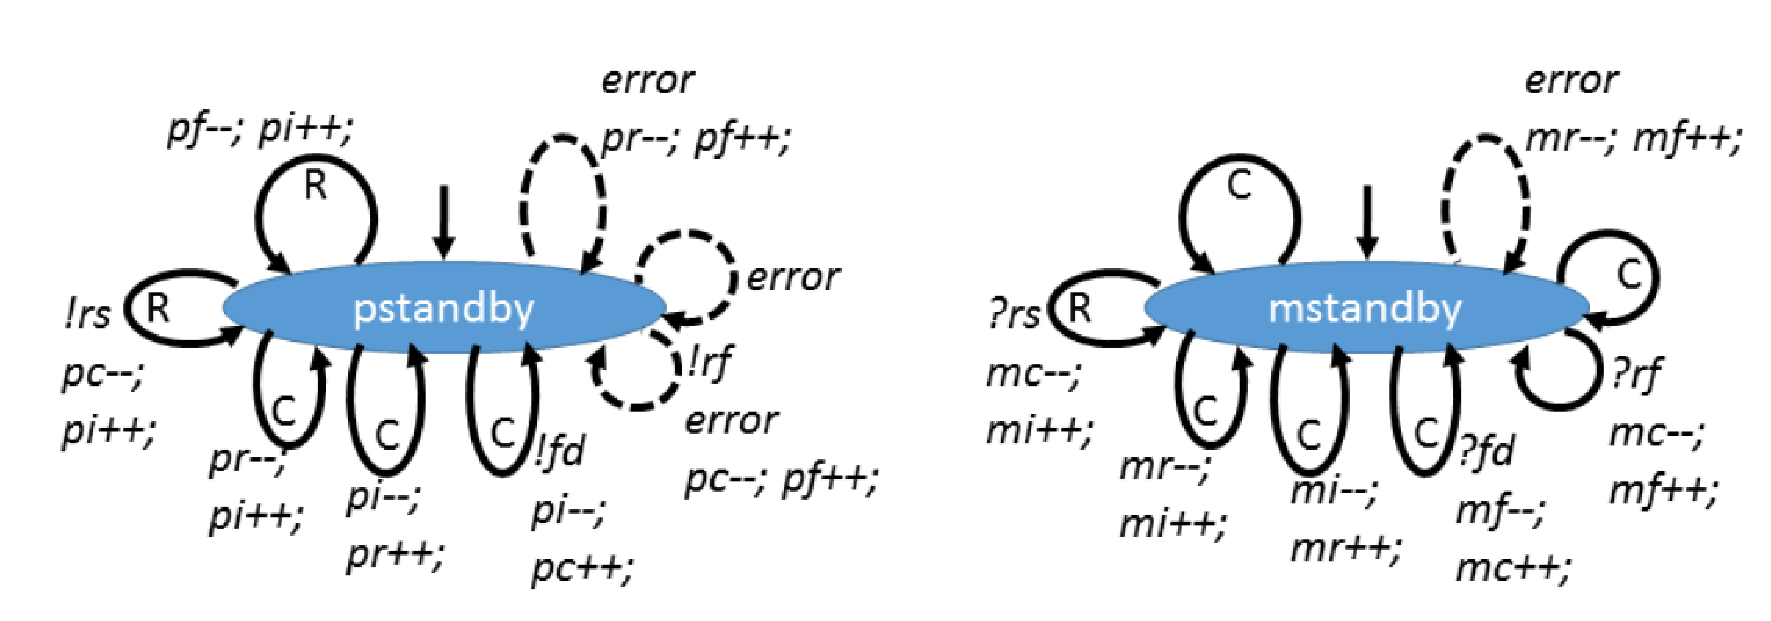
\epsfig{file=aviC.eps,width=140mm} 
\caption{Counter abstraction of the CEFSM templates of $n$ processors and $m$ memory copies}
\label{fig.pmC}
\end{center} 
\end{figure*}
The initial state are specified with constraint: 
$\mbox{\em pr}=n
\wedge \mbox{\em pi}=0
\wedge \mbox{\em pc}=0
\wedge \mbox{\em pf}=0
\wedge \mbox{\em mr}=m
\wedge \mbox{\em mi}=0
\wedge \mbox{\em mc}=0
\wedge \mbox{\em mf}=0$
on the counters.  
The state in the product automata must satisfy the following constraints: 
$\mbox{\em pr}+\mbox{\em pi}+\mbox{\em pc}+\mbox{\em pf}=n
\wedge \mbox{\em mr}+\mbox{\em mi}+\mbox{\em mc}+\mbox{\em mf}=m$.  
As can be seen, we do not care which processor is in the idle mode, 
in the running mode, etc., in this abstraction. 
Similarly, we do not care which memory module is in the idle mode, in the running mode, and etc. 
The local state transition only keeps tracks of the number of processors in each mode and 
the number of memory modules in each mode. 
We also do not care which processor is in charge of the recovery of which memory module.  
Such an abstraction can be done automatically.  

The labeling of the move vectors on the transitions in the Kripke structure (product automaton)
follows the same rules for the product automaton from the CEFSM in Figure~\ref{fig.pm}.  




\subsection*{Analysis of the game structure} 
The majority outcome of the processors and memory copies 
is used as the outcome of the system.  
A processor may enter the faulty state.  
A memory module may also enter the faulty state. 
Processors may control to recover themselves or a faulty memory module 
by copying the contents of a functioning memory module to 
the faulty one.  
At any moment, we want to make sure that we can always recover 
to a global condition with the following two restrictions. 
\begin{itemize} 
\item There are at least two more processors in \label{reply2.2more} 
	the running mode than the processors in the faulty mode.  
\item There are at least two more memory copies in 
	the running mode than memory copies in the faulty mode. 
\end{itemize} 
Together, the failure condition is 
$\textit{crp}-\textit{cfp}<2\vee\textit{crm}-\textit{cfm}<2$.  
That is, all states in the transition system satisfying 
$\textit{crp}-\textit{cfp}<2\vee\textit{crm}-\textit{cfm}<2$ 
are in set $F$.  

We report the performance data 
in Table~\ref{tab.perf} for the resilience algorithms 
described in Section~\ref{subsec.bench} 
against the parameterized benchmarks in the above with various 
parameters.  
The second column shows the concurrency sizes.  
The third column shows the values of $k$ for the rows.  
The fourth and fifth columns show the sizes of the concurrent game structures.  
The sixth and seventh columns show the time and spaces used to calculate 
sfrch$_k()$.  
Similarly, the eighth and ninth columns show the time and spaces for calculating 
the res$_k()$.  

The benchmark in Figure~\ref{fig.pm} does not have nodes in 
$\safe_2(G)$ and $\res_2(G)$.  
So we changed the benchmark to see how we check our implementation 
with $k>1$.  
The change is that the recovery transition from state \textit{pcopy} to 
\textit{pidle}
of processors are relabeled as controllable. 
This change significantly limits the ability of the system errors 
to derail the system.  
\begin{table*}[t] 
\caption{Performance data for resilience calculation \hspace{21mm} s: seconds; M: megabytes} 
\label{tab.perf} 
\begin{center} 
\resizebox{\columnwidth}{!}{
\begin{tabular}{l|c|c|c|c||c|c||c|c} \hline 
benchmarks & concurrency & $k$ & \multicolumn{2}{c||}{game sizes} 
& \multicolumn{2}{c||}{sfrch$_k$}  
			& \multicolumn{2}{c}{res$_k$} \\\cline{4-9} 
	 & 	& & \#nodes & \#edges & time  & memory   & time & memory  \\
\hline \hline 
avionics & 2 processors \& 2 memory modules 
     & 2 & 118 & 750 
     & 0.62s & 114M & 0.85s & 116M \\ \cline{2-9} 
     & 2 processors \& 3 memory modules 
     & 2 & 414 & 3252
     & 0.94s & 139M & 1.10s & 153M \\ \cline{2-9} 
     & 3 processors \& 3 memory modules 
     & 3 & 1540 & 15090 
     & 4.67s & 225M & 8.38s & 267M \\ \cline{2-9} 
     & 3 processors \& 4 memory mdules
     & 3 & 5601 & 63889 
     & 42.86s & 815M & 155s & 846M \\ \hline  
avionics & 6 processors \& 6 memory modules 
	 & 2 & 1372 & 6594 
	 & 2.89s & 129M & 3.54s & 516M \\ \cline{2-9} 
(counter	 & 7 processors \& 7 memory modules 
	 & 3 & 2304 & 11396 
	 & 10.7s & 216M & 23.4s & 808M \\ \cline{2-9}
abstraction)	 & 8 processors \& 8 memory modules 
	 & 3 & 3645 & 18432 
	 & 43.8s & 1009M & 135s & 2430M \\ \hline 
voting	 & 1 client \& 20 replicas 
	 & 9 & 9922 & 23551 & 7.01s & 260M & 36.7s & 297M \\ \cline{2-9} 
	 & 1 client \& 26 replicas 
	 & 12 & 20776 & 49882 & 19.9s & 474M & 79.6s & 611M \\ \hline 
simple	 & 1 client \& 150 replicas 
	 & 74 & 458 & 1056 & 0.71s & 159M & 31.7s & 219M \\ \cline{2-9} 
voting	 & 1 client \& 200 replicas 
	 & 99 & 608 & 1406 & 1.06s & 161M & 162s & 337M \\ \cline{2-9} 
	 & 1 client \& 250 replicas 
	 & 124 & 758 & 1756 & 1.36s & 163M & 307s & 499M \\ \hline 
PBFT 	 & 1 client \& 6 replicas 
	 & 2 & 577 & 897 & 0.34s & 72M & 1.05s & 193M \\ \cline{2-9} 
	 & 1 client \& 9 replicas 
	 & 4 & 2817 & 4609 & 13.3s & 564M & 58.5s & 1657M \\ \hline 
clock	 & 1 client \& 15 servers  
	 & 7 & 16384 & 229376 & 45.1s & 3075M & 62.4s & 3264M  \\ \cline{2-9} 
sync	 & 1 client \& 17 severs  
	 & 8 & 65536 & 1070421 & 870s & 14725M & 915s & 15433M  \\ \hline 
\end{tabular}
}
\end{center}
\vspace*{-5mm}
\end{table*}
For the avionics system, %the $k$ value
the resilience level $k$ is set to 
one less than half the %value
number of processors.  
For the voting and simple voting benchmarks, 
the value of $k$ is set to one less than half the number of 
replicas (voters). 
For the PBFT and clock synchronization algorithm, we choose 
$k$ to be one less than one third of the number of replicas. 

The performance data has been collected with a Virtual Machine (VM) 
running opensuse 11.4 x86 
on Intel i7 2600k 3.8GHz CPU 
with 4 cores and 8G memory. 
The VM only uses one core and 4G memory.  

The time and space used to calculate resilience is a little bit more 
than that to check for $\safe$.  
The reason is that $\safe_k$ is a pre-requisite for calculating $\res_k$.  
In our experiment, $\safe_k$ is usually 
very close to $\res_k$ and does not require much extra time in 
calculating $\res_k$ out of $\safe_k$.  

The experiments show that our techniques 
scale to realistic levels of redundancy.  
For fault-tolerant hardware, usually the numbers of replicas are small, 
for example, less than 10 replicas. 
Thus our techniques seem very promising for the 
verification and synthesis\label{reply2.verification.hardware} of hardware fault-tolerance.  

On the other hand, 
nowadays, software fault-tolerance through networked computers can 
create huge numbers of replicas.  
Our experiment shows that counter abstraction can be a useful 
techniques for the modeling and verification of software resilience.  
Specifically, for the avionics benchmark, 
we can verify models of much higher concurrency and complexity with 
counter abstraction than without. 
% As can be seen, our techniques can really prove the % safety and 
% resilience of pretty large concurrency sizes.  



\chapter{Conclusions}
\label{c:conclusions}
%\chapter{Theory of surface plasmon polaritons in metallic nano-structures}
\label{c:thm}
\section{Definition of plasmon}

Plasmon is collective oscillation of conduction electron gas, a quasi-particle resulting from the quantization of plasma oscillations just like phonons are quantizations of mechanical vibrations. The simplest case is the volume plasmon as shown in Figure~\ref{fig:bulk}.
\begin{figure}[htb]
\centering
\includegraphics[scale=0.5]{THM/bulk.eps}
\caption{\label{fig:bulk}Longitudinal collective oscillations of the conduction electrons of a metal (Volume plasmons)}
\end{figure}
 We can derive plasma frequency $\omega_p$ from the simple harmonics oscillation model, a collective displacement of the electron cloud by a distance $u$ leads to a surface charge density $\sigma = \pm neu$ at the slab boundaries. This establishes a homogeneous electric field $\mathbf{E} = \frac{neu}{\varepsilon_0}$ inside the slab. Thus, the displaced electrons experience a restoring force, and their movement can be described by the equation of motion $nm\ddot{u} = -ne\mathbf{E}$. Inserting the expression for the electric field, this leads to
 \begin{subequations}
 \begin{align}
 nm\ddot{u} = -\frac{n^2e^2u}{\varepsilon_0} \\
 \ddot{u} + {\omega_p}^{2}u = 0\text{.}
 \end{align}
 \end{subequations}
  The plasma frequency $\omega_p = \sqrt{\frac{ne^2}{\varepsilon_0m}}$ can thus be recognized as the natural frequency of a free oscillation of the electron sea. The quanta of these charge oscillations are called plasmons. Due to the longitudinal nature of the excitation, volume plasmons do not couple to transverse electromagnetic waves, and can only be excited by particle impact. We can derive the dispersion relation of the generalization of volume plasmons, traveling plasma waves, from curl electric field equations (Equations~\ref{eq:curlE})
 \begin{subequations}
 \begin{align}
 \curl{\curl \mathbf{E}} &= -\mu_0 \frac{\partial^2\mathbf{D}}{\partial t^2}\label{eq:curlE}\\
\mathbf{K}( \mathbf{K}\cdot \mathbf{E}-K^{ 2 }\mathbf{E} ) &=-\varepsilon ( \mathbf{K},\omega  ) \frac { { \omega  }^{ 2 } }{ { c }^{ 2 } } \mathbf{E}
 \end{align}
 \end{subequations}  
and plasma model, and a simple equation of motion for an electron of the plasma subjected to an external electric field $\mathbf{E}$
 \begin{equation}
m\ddot{\mathbf{x}} + m\gamma\dot{\mathbf{x}} = -e\mathbf{E}\text{.}
\end{equation}
Assuming a harmonic time dependence $\mathbf{E}( t )=\mathbf{E}_0\mathrm{e}^{-i\omega t}$ of the driving field, a particular solution of this equation describing the oscillation of the electron is $\mathbf{x} ( t ) = \mathbf{x}_0 \mathrm{e}^{-i\omega t} $. The complex amplitude $\mathbf{x}_0$ incorporates any phase shifts between driving field and response via
\begin{equation}
\mathbf{x} ( t ) = \frac{e}{m( \omega^2 + i\gamma\omega )}\mathbf{E}( t )\text{.}
\end{equation}
The displaced electrons contribute to the macroscopic polarization
\begin{equation}
\mathbf{P}=-\frac{ne^2}{m( \omega^2 + i\gamma\omega )}\mathbf{E}( t )\text{.}
\end{equation}
Inserting $\mathbf{P}$ into dielectric displacement field equation $\mathbf{D} = \varepsilon_0\mathbf{E} + \mathbf{P}$ yields
\begin{equation}
\mathbf{D} = \varepsilon_0(1-\frac{\omega_p^2}{\omega^2 + i\gamma\omega})\mathbf{E}\text{,}
\end{equation}
where $\omega_p^2 = \frac{ne^2}{\varepsilon_0m}$. Therefore, the dielectric function of the free electron gas
\begin{equation}
\varepsilon(\omega) = 1- \frac{\omega_p^2}{\omega^2 + i\gamma\omega}\text{.}\label{eq:dielefu}
\end{equation}
We arrive at the desired result by using equation~\ref{eq:dielefu} and the generic dispersion relation $K^2=\varepsilon(\mathbf{K},\omega)\frac{\omega^2}{c^2}$, the dispersion relation of traveling waves becomes
\begin{equation}
\omega^2 = \omega_p^2 + \mathbf{K}^2c^2\text{.}
\end{equation}
From this relation, we can figure out the oscillation properties in any frequency of external field. Note that this branch can not confine the electromagnetic waves, it would radiate out the energy, so this mode is also called radiative surface plasmon.

\section{Surface plasmon polaritons at interface between dielectric and metal}

Surface plasmon polaritons (SPPs) are eigenmodes of transverse magnetic (TM) waves, which coupling the electromagnetic fields to oscillations of the conductor's electron plasma, propagate at a interface between dielectric and metal, and are confined in perpendicular direction. Providing a flat interface between dielectric and metal half-spaces with dielectric constants $\varepsilon_d$ and $\varepsilon_m$ , respectively, and assuming the interface normal to z direction and the SPPs propagate along the $x$ direction, the SPP wave vector $\beta$ is related to the frequency $\omega$ through the dispersion relation
\begin{equation}
\beta = k_0\sqrt{\frac{\varepsilon_d\varepsilon_m}{\varepsilon_d + \varepsilon_m}}\text{,}\label{eq:sppsdisp}
\end{equation}
where $k_0 = \omega/c$ is the free-space wave vector. We take $\omega$ to be real and allow $\beta$ to be complex.

The optical response of metals is often described by the Drude model for a free-electron gas~\cite{kittel1976introduction},
\begin{equation}
\varepsilon_{Drude}(\omega)=1-\frac{\omega_p^2}{\omega^2+i\Gamma\omega}\text{,}
\end{equation}
in which $\Gamma$ is a damping rate due to electron-electron and electron-phonon scattering.
Figure~\ref{fig:SPPdisp} shows the dispersion curve~\ref{eq:sppsdisp} with Drude metal  in the absence of losses ($\Gamma=0$) for air ($\varepsilon_d = 1$) and fused silica ($\varepsilon_d = 2.25$) interface.
\begin{figure}[htb]
\centering
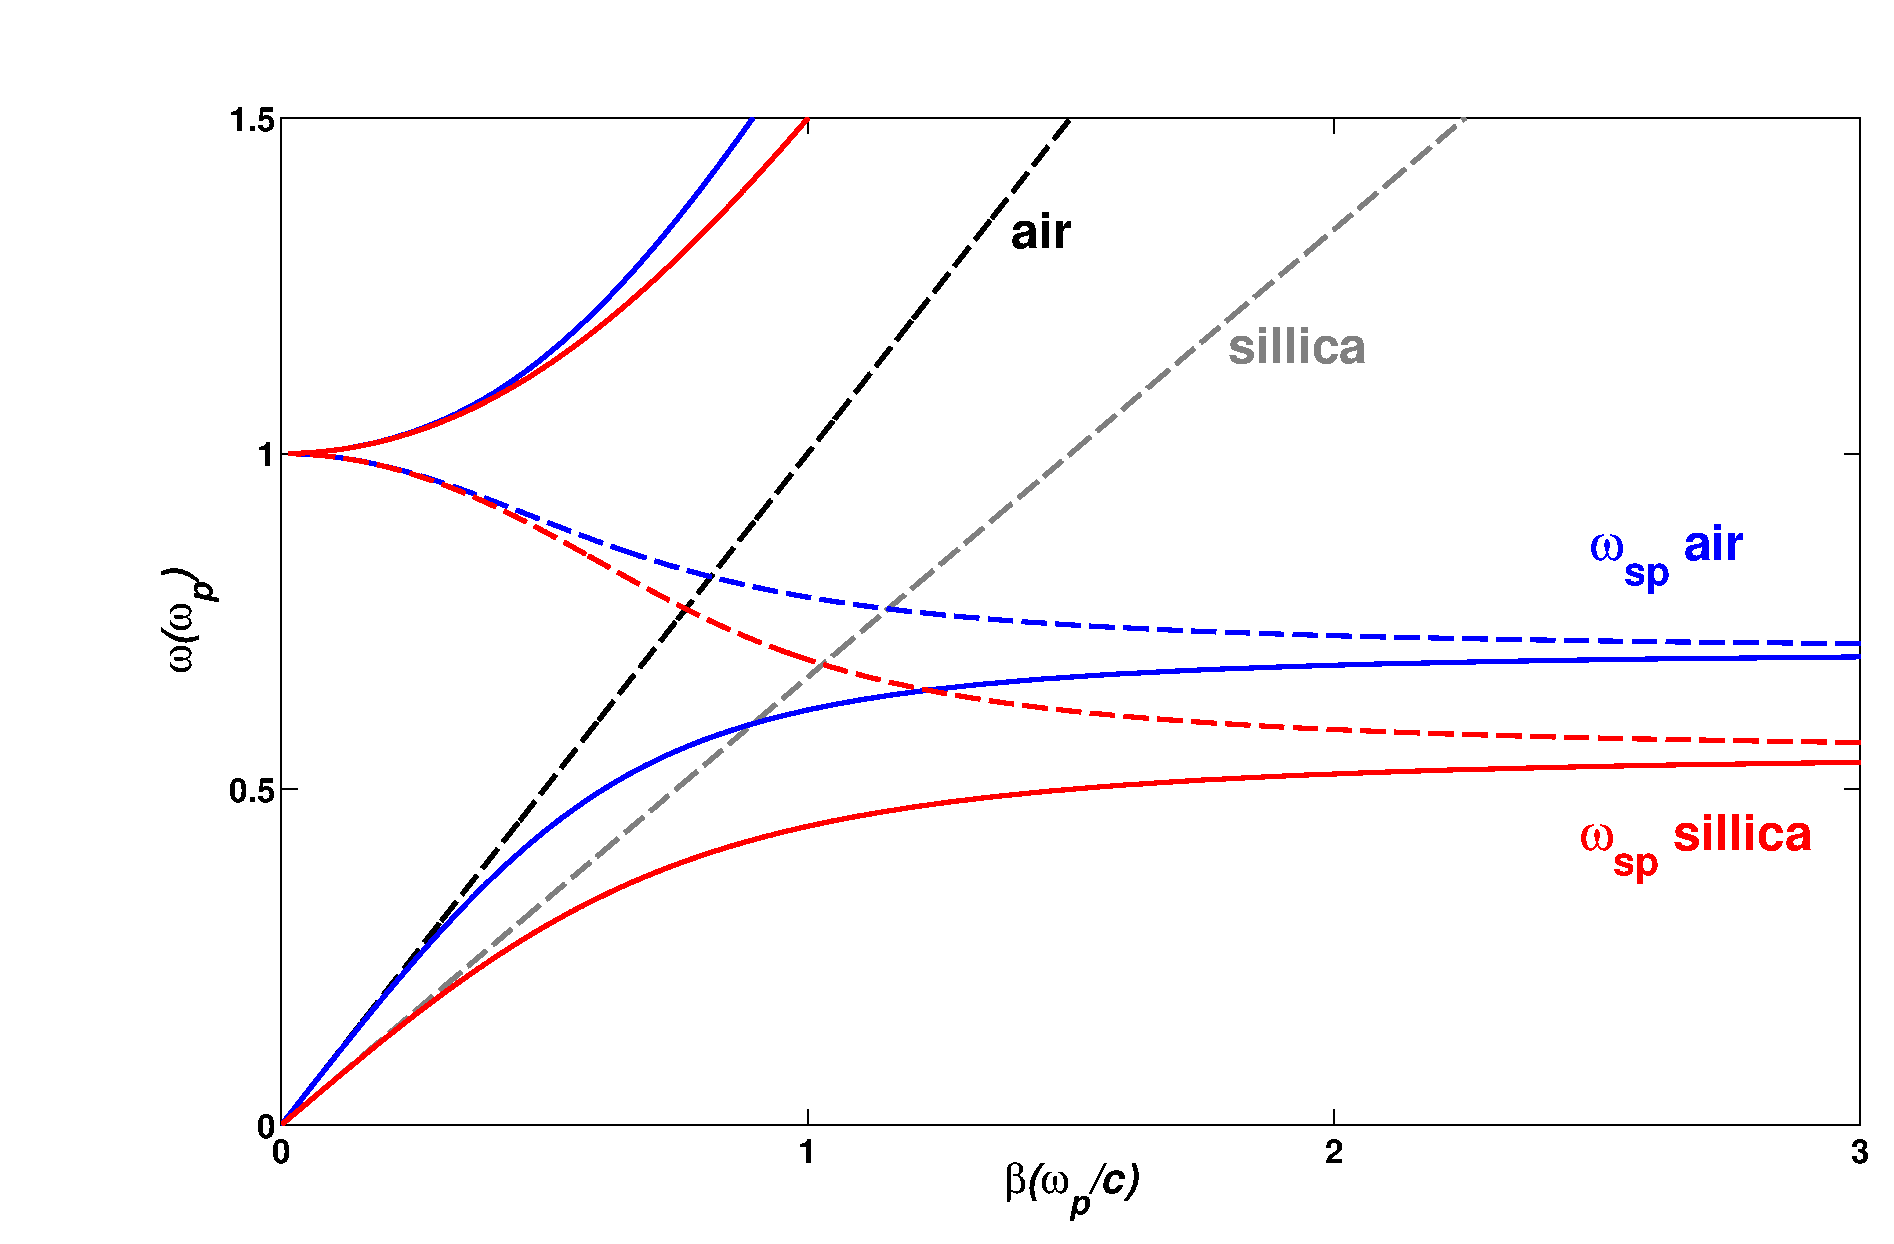
\includegraphics[scale=0.4]{THM/SPPdisp.eps}
\caption{\label{fig:SPPdisp}Dispersion relation of SPPs at the interface between a Drude metal with negligible collision frequency and air (blue curves) and silica (red curves).}
\end{figure}
For small wave vectors SPPs propagation constant $\beta$ is close to $k_0$ at the light line, in the opposite regime of the frequency close to surface plasmon frequency $\omega_p$. It also shows that the SPPs line lying to the right of the respective light lines of air and silica, so that SPPs are directed by light due to phase mismatching. The wave vector mismatch between SPPs and radiation modes needs to be overcome in order to excite or detect SPPs. This can be achieved by multiple methods~\cite{raether1988surface}. In the Otto configuration, light in a prism that is brought in close vicinity to a metal surface can excite SPPs through coupling to the evanescent field. Because light in the prism has a larger wave vector than that in air, it can be phase-matched to the SPPs. In the related Kretschmann-Raether geometry, coupling to SPPs occurs through a metal film that is deposited on a prism. In the grating coupling configuration, metal surface with a shallow grating of grooves or holes with lattice constant $a$. For the simple 1D grating of grooves depicted in Figure~\ref{fig:grating},
\begin{figure}[htb]
\centering
\includegraphics[scale=0.5]{THM/grating.eps}
\caption{\label{fig:grating}Phase-matching of light to SPPs the grating coupling configuration.}
\end{figure}
phase-matching takes place when the condition is fulfilled
\begin{equation}
\beta = k_0 \sin{\theta} \pm \nu g\text{,}
\end{equation}
where $g=\frac{2\pi}{a}$ is the reciprocal vector of the grating, and $\nu=(1,2,3\dots)$.
As with prism coupling, excitation of SPPs is detected as a minimum in the reflected light. The reverse process can also take place, SPPs propagating along a surface modulated with a grating can couple to light and thus radiate. 

%\bibliographystyle{unsrt}
%\bibliography{thesisbib}
%\input{main}

%chapter cite  == \include

%\chapter{Get started with \LaTeX\ }
\label{c:GetStarted}
Two common font styles in this text: 
\begin{itemize}
    \item \textbf{Item1}: \textit{Italic}     
    \item \textbf{Item2}: \textbf{Bold}
\end{itemize}

About the advance latex grammer see the next section \ref{s:AdvancedFeatures}.


\section{\LaTeX\ Adavanced Features}
\label{s:AdvancedFeatures}
The following features would be introduced in the coming subsections:
\begin{itemize}
    \item SubSection \ref{ss:Figure}: \hyperref[ss:Figure]{\textbf{Figure}}
    \item SubSection \ref{ss:VerbUsage}: \hyperref[ss:VerbUsage]{\textbf{Verb}}
    \item SubSection \ref{ss:VerbUsage}: \hyperref[ss:VerbUsage]{\textbf{Verb}}
    \item SubSection \ref{ss:Enumeration}: \hyperref[ss:Enumeration]{\textbf{Enumeration}}
    \item SubSection \ref{ss:Table}: \hyperref[ss:Table]{\textbf{Table}}
    \item SubSection \ref{ss:CodeDisplay}: \hyperref[ss:CodeDisplay]{\textbf{Code Display}}
    \item SubSection \ref{ss:Math}: \hyperref[ss:Math]{\textbf{Math}}
    \item SubSection \ref{ss:Algorithms}: \hyperref[ss:Algorithms]{\textbf{Algorithms}}
\end{itemize}

%==========================================================================================
\subsection{Figure}
\label{ss:Figure}
\begin{figure}[htpb!]
  \centering
    \includegraphics[width=0.5\textwidth]{fig/tiger.jpeg}
    \caption{\label{fig:tiger}A picture of a tiger.}
\end{figure}

Figure~\ref{fig:tiger} is a picture of a tiger.


%==========================================================================================
\subsection{Table}
\label{ss:Table}

\href{http://en.wikibooks.org/wiki/LaTeX/Tables}{Table examples on WIKIBOOKS}.

\begin{table}[htpb]\begin{center}
\caption{Table Example 1}
\begin{tabularx}{8cm}{llX}
\hline
Start & End  & Character Block Name \\
\hline
3400  & 4DB5 & CJK Unified Ideographs Extension A \\
4E00  & 9FFF & CJK Unified Ideographs \\
\hline
\end{tabularx}
 \end{center}\end{table}

\begin{table}[htpb]\begin{center}
\caption{Table Example 2}
\begin{tabular}{llr}
\hline
\multicolumn{2}{c}{Item} \\
\cline{1-2}
Animal & Description & Price (\$) \\
\hline
Gnat  & per gram & 13.65 \\
      & each     &  0.01 \\
Gnu   & stuffed  & 92.50 \\
Emu   & stuffed  & 33.33 \\
Armadillo & frozen & 8.99 \\
\hline
\end{tabular}
 \end{center}\end{table}
 
 \begin{table}[htpb]\begin{center}
	\label{t:prefix-table}
	\caption{Table Example 3}
	\renewcommand{\arraystretch}{1.0}
	\begin{tabularx}{300pt}{|c|X| }
		\hline
		\multirow{1}{*}{\textbf{Allocation}} &
		Allocation, Element, Type, Script 
		\\ \hline\hline
		%------------------------------
		\multirow{6}{*}{\textbf{Data Types}} &
        Byte2, Byte3, and Byte4\\ &
        Float2, Float3, Float4\\ &
        Int2, Int3, Int4\\ &
        Long2, Long3, Long4\\ &
        Matrix2f, Matrix3f, Matrix4f\\ &
        Short2, Short3, Short4
        \\ \hline\hline
		%------------------------------
		\multirow{4}{*}{\textbf{Graphics}} &
		Mesh\\&
		ProgramFragment, ProgramRaster\\&
		ProgramStore, ProgramVertex\\&
		RSSurfaceView
		\\ \hline
		%------------------------------
	\end{tabularx}
\end{center}\end{table}

\begin{table}[htpb]\begin{center}
\caption{Table Example 4}
\begin{tabular}{|l|l|l|}
\hline
\multicolumn{3}{|c|}{Team sheet} \\
\hline
Goalkeeper & GK & Paul Robinson \\ \hline
\multirow{4}{*}{Defenders} & LB & Lucus Radebe \\
 & DC & Michael Duberry \\
 & DC & Dominic Matteo \\
 & RB & Didier Domi \\ \hline
\multirow{3}{*}{Midfielders} & MC & David Batty \\
 & MC & Eirik Bakke \\
 & MC & Jody Morris \\ \hline
Forward & FW & Jamie McMaster \\ \hline
\multirow{2}{*}{Strikers} & ST & Alan Smith \\
 & ST & Mark Viduka \\
\hline
\end{tabular}
 \end{center}\end{table}
 
 \begin{table}[htpb]\begin{center}
\caption{Table Example 5}
 \begin{tabular}{l*{6}{c}r}
Team              & P & W & D & L & F  & A & Pts \\
\hline
Manchester United & 6 & 4 & 0 & 2 & 10 & 5 & 12  \\
Celtic            & 6 & 3 & 0 & 3 &  8 & 9 &  9  \\
Benfica           & 6 & 2 & 1 & 3 &  7 & 8 &  7  \\
FC Copenhagen     & 6 & 2 & 1 & 2 &  5 & 8 &  7  \\
\end{tabular}
 \end{center}\end{table}

%==========================================================================================
\subsection{Verb}
\label{ss:VerbUsage}
Let's take a overview on how to type special characters:\\
\verb|<FRAMEWORKS_BASE>/graphics/java/android/renderscript|\\\footnote{Path of <APP\_intermediates>: <ANDROID\_ROOT>/out/target/common/obj/APPS/APPNAME\_intermediates/}
You could also go back to the beginning of the chapter by the \hyperref[c:GetStarted]{\textbf{hyperref}}.

%==========================================================================================
\subsection{Enumeration}
\label{ss:Enumeration}
\begin{enumerate}
\item Enumerated Item1
\item Enumerated Item2
\item Enumerated Item3
\end{enumerate}

%==========================================================================================
\subsection{Code Display}
\label{ss:CodeDisplay}

\lstset{
	language=C++,
	stringstyle=\rmfamily,
	commentstyle=\itshape\color[rgb]{0.133,0.545,0.133},
	showstringspaces=false,
	basicstyle=\ttfamily\scriptsize,
	numberstyle=\tiny,
	numbers=left,
	stepnumber=1,
	numbersep=10pt,
	tabsize=2,
	breaklines=true,
	prebreak = \raisebox{0ex}[0ex][0ex]{\ensuremath{\hookleftarrow}},
	breakatwhitespace=false,
  	columns=fixed,
  	upquote=true,
  	extendedchars=true,
	xleftmargin=2em,
	xrightmargin=.5em,
	escapeinside={(*@}{@*)},
    mathescape=false,
}
Here is a "Hello, DanDing." example:
\begin{lstlisting}[style=nonumbers] 
void main(int argc, char **argv)
{
    printf("   ˊ_> ˋ  ");
}
\end{lstlisting}


Another example with line numbers:
\begin{lstlisting}
void main(int argc, char **argv)
{
    printf("   ˊ_> ˋ  ");
}
\end{lstlisting}

Matlab example:

\definecolor{dkgreen}{rgb}{0,0.6,0}
\definecolor{gray}{rgb}{0.5,0.5,0.5}
\lstset{language=Matlab,
   keywords={break,case,catch,continue,else,elseif,end,for,function,
      global,if,otherwise,persistent,return,switch,try,while},
   basicstyle=\ttfamily,
   keywordstyle=\color{blue},
   commentstyle=\color{red},
   stringstyle=\color{dkgreen},
   numbers=left,
   numberstyle=\tiny\color{gray},
   stepnumber=1,
   numbersep=10pt,
   backgroundcolor=\color{white},
   tabsize=4,
   showspaces=false,
   showstringspaces=false}

\begin{lstlisting}
function y = demo(x) % This is a comment.
   str = 'hello there';
   y = x + 1;
end
\end{lstlisting}

%==========================================================================================
\subsection{Math}
\label{ss:Math}
\begin{itemize}
    \item Inline mode:\\
The solution to $\sqrt{x} = 5$ is $x=25$.
    \item Display mode:\\
The solution to \[\sqrt{x} = 5\] is \[x=25.\]
    \item Numbered mode:
\begin{equation}
2+2=4
\end{equation}
    \item Non-numbered:
\begin{equation*}
2+2=4
\end{equation*}
    \item Aligning:
\begin{align*}
2x^2 + 3(x-1)(x-2) & = 2x^2 + 3(x^2-3x+2)\\
&= 2x^2 + 3x^2 - 9x + 6\\
&= 5x^2 - 9x + 6
\end{align*}
     \item Fractions:
\[
 \frac{n!}{k!(n-k)!} = \binom{n}{k}
\]
    \item Matrix:
\[
 A_{m,n} =
 \begin{pmatrix}
  a_{1,1} & a_{1,2} & \cdots & a_{1,n} \\
  a_{2,1} & a_{2,2} & \cdots & a_{2,n} \\
  \vdots  & \vdots  & \ddots & \vdots  \\
  a_{m,1} & a_{m,2} & \cdots & a_{m,n}
 \end{pmatrix}
\]
\end{itemize}
\href{http://en.wikibooks.org/wiki/LaTeX/Mathematics}{More examples on WIKIBOOKS}.


%==========================================================================================
\subsection{Algorithms}
\label{ss:Algorithms}
\begin{algorithm}[h]                      % enter the algorithm environment
\caption{Calculate $y = x^n$}          % give the algorithm a caption
\label{alg1}                           % and a label for \ref{} commands later in the document
\begin{algorithmic}                    % enter the algorithmic environment
    \Require $n \geq 0 \vee x \neq 0$
    \Ensure $y = x^n$
    \State $y \Leftarrow 1$
    \If{$n < 0$}
        \State $X \Leftarrow 1 / x$
        \State $N \Leftarrow -n$
    \Else
        \State $X \Leftarrow x$
        \State $N \Leftarrow n$
    \EndIf
    \While{$N \neq 0$}
        \If{$N$ is even}
            \State $X \Leftarrow X \times X$
            \State $N \Leftarrow N / 2$
        \Else[$N$ is odd]
            \State $y \Leftarrow y \times X$
            \State $N \Leftarrow N - 1$
        \EndIf
    \EndWhile
\end{algorithmic}
\end{algorithm}
\href{http://en.wikibooks.org/wiki/LaTeX/Algorithms_and_Pseudocode}{More examples on WIKIBOOKS}.


%\chapter{Introduction}
\label{c:intro}

There can be million lines of code in today's software system.
On such a scale of complexity, defects in the source codes are unavoidable.  
Various empirical studies show that the defect density of commercial software system is around 1 to 20 defects in every 1000 lines of source code\cite{Sommerville:2006:SE:1196763}.
Therefore, developers of systems created many engineering techniques to contain the damage that could be caused by such defects.
For example, a software system may have several measures to its disposal to avoid system failure, including resending the request, resetting the server, clearing the communication buffers, and etc when observing that a critical service request is not acknowledged.
However, in general, since all the recovery cost time and money it is important to estimate how to organize the measures for the maximal resilience of the system against realistic errors.
At the moment, an automated support which can suggest defence techniques to development teams is missing.
I created a game theoretic approach to study this problem and carried out experiments to show how this approach can be helpful in  synthesizing the most resilient defence of software systems against multiple errors.

The naive way to measure the safety level of a system is to find the number of errors that it can endure before running into failure state.
But in second thought, no non-trivial system can handle unlimited errors without degrading to inevitable system failure.
Thus, it would be meaningless to analyse the resilience level of the systems to software errors can proceed without creating a realistic error model in which practical control mechanism can be devised to defend the systems against errors.
In this work, I am interested in defending the system against a more restricted error model, but still let the error model has a quantifiable level of power in order to simulate different error scenarios.
Further more, I think a reasonable foundation need to take into consider that the life-time of a software system is much longer than the duration needed for a reasonably designed software system to recover from an error.
Therefore, I propose to evaluate control mechanism of software systems on how many errors the control can endure before recovery to safe states.
I then present an algorithm to find a control strategy that can handle the maximum number of such errors.

Let us standardize the basic terms before proceeding further.
A design defect in software or hardware is called a {\it fault} in embedded systems.
An {\it error} (sometimes called component failure in the literature) is the effect of a fault that causes a difference between the expected and the actual behavior of a software system, e.g., measurement errors, read/write errors, etc. 
An {\it error} does not always lead to a system failure, but may instead be repaired by, e.g., a defence mechanism in the software. 
That is, an {\it error} may be detected and fixed/neutralized before it creates any harm to the system or its users.
A {\it failure} is the fact that users can observe the faulty behavior created by {\it errors}.

My specific goal is to develop a technique for finding a control mechanism of a software system which can against the maximal number of dense errors without degrading to failure.
My inspiration is from methods for resilient avionic systems\cite{conf/ftrtft/1992}, where fault tolerance is designed to recover from a bounded number of errors.
The number of errors a system needs to tolerate is calculated from the mean time between errors of individual components and the maximal duration of the system.
I use the quality guarantees one obtains for an airplain(the system) as an example to demonstrate the difference between the objective to tolerate up to {\it k errors} and sequences of separated blocks of up to {\it k dense errors} in a short period.
Assuming the operating time of the system is 20 hours, the mean time between exponentially distributed errors is 10 hours and the repair time is 3.6 seconds.
The mean time between dense errors (consecutive errors before system recovery) is calculated in Table~\ref{tab.mtbf}.
\begin{table*}
\begin{center}
\resizebox{\columnwidth}{!}{
\begin{tabular}{l||c|c|c|c|c|c|c|c}\hline 
$k$              & $0$     & $1$     &    $2$   &  $3$  & $4$ & $5$ & $6$ & $\ldots$ \\\hline 
$k$ errors       & $0.865$ & $0.594$ & $0.333$ & $0.143$ & $0.053$ & $0.017$ & $0.005$ & $\ldots$ \\
$k$ dense errors & $0.865$ & $2 \cdot 10^{-4}$ & $2 \cdot 10^{-9}$ & $2 \cdot 10^{-14}$ & $2\cdot 10^{-19}$ & $2\cdot 10^{-24}$ & $2\cdot 10^{-29}$ & $\ldots$ 
\\ \hline 
\end{tabular}
}
\end{center}
\caption{Probabilities of $k$ dense errors} 
\label{tab.mtbf} 
\end{table*} 
%\bibliographystyle{unsrt}
%\bibliography{thesisbib}
The figures for $k$ errors (component failures) are simply the values 
for the Poisson distribution with coefficient $2$.
To explain the figures for $k$ dense errors, 
consider the density of 2 dense errors occurring in close succession.
If an error occurs, the chance that the next error occurs 
within the repair time (3.6 seconds) is approximately $\frac{1}{10000}$.
The goal to tolerate an arbitrary number of up to $k$-dense errors is, of course, 
much harder than the goal of tolerating up to $k$ errors, but, 
as the example shows, the number $k$ can be much smaller.   
Tolerating an arbitrary number of errors 
(with a distance of at least $3.6$ seconds between them) 
creates the same likelihood to result in a system failure 
as tolerating up to $9$ errors overall, and 
tolerating up to $15$ errors still results 
in a $70\%$ higher likelihood of a system failure 
than tolerating blocks of up to $2$ errors in this example. 
Only errors for which this is the case could cause a system failure.
The mean time between blocks of two dense errors is therefore not ten hours, 
but 100,000\label{reply2.100000} hours.
Likewise, it increases to 1,000,000,000 (one billion) hours for blocks of three dense errors, and so forth.

Maximizing the number of dense errors that are permitted before full recovery 
is therefore a natural design goal.  
After full recovery, the system is allowed again the same number of errors.
Now, if the {\em mean time between errors} ({\em MTBE}) 
is huge compared to the time the system needs to fully recover, 
then the mean time between system failures (MTBF) grows immensely. 

We view the problem of designing a resilient control mechanism 
towards dense errors as a two-player game, 
called {\em safety resilience game}, 
between the system (\label{reply1.protagonist.player1}protagonist\footnote{In game theory, a protagonist sometimes is also called {\em player 1}.}, `he' for convenience) 
and a hostile agent (antagonist\footnote{In game theory, an antagonist sometimes is also called {\em player 2}.}, `she' for convenience) 
that injects errors into the system under execution.\label{reply1.antagonist.inject.errors}   
The protagonist wants to keep the system from failure in the presence of errors, 
while the antagonist wants to derail the system to failure. 
\label{reply1.how.models} 
Specifically, 
system designers may model their system, defense mechanism, and error model 
as a finite game graph.  
The nodes in the graph represent system states.
These system states are partitioned into three classes:
the safe states, the failure states, and the recovery states. 
Some transitions are labeled with errors while others are considered normal transitions.  
The game is played with respect to a resilience level $k$.  
If a play ever enters a failure state, then the antagonist wins in the play.  
Otherwise, the protagonist wins.

The protagonists plays by selecting a move, intuitively the `normal' event that should happen next (unless an error is injected).
The antagonist can then decide to trigger 
an error transition (injecting an error) with the intention to
eventually deflect the system into a failure state. 
Our error model, however, restricts 
the antagonist to inject at most $k$ errors before she allows for a long period of time that the system may use to recover to the safe states.
(If the antagonist decides to use less than $k$ errors, the protagonist does not know about this.
It proves that this information is not required, as we will show
\label{reply1.memoryless.future} that the protagonist can play memoryless.)
After full recovery by the protagonist to the safe states, the antagonist is allowed again 
to inject the same number of errors, and so forth.
  
If the system can win this game, then the system is called {\em $k$-resilient}.
For $k$-resilient systems, there exists a control strategy---even one that does not use memory---to make the system 
resilient in the presence of blocks of up to $k$ dense errors. 
We argue that, if the component MTBF is huge compared to the time the system needs to fully recover, then the expected time for system breakdown grows immensely.  

Besides formally defining safety resilience games, we also present algorithms 
for answering the following questions.  
\label{reply2.alg.sfrch.res}
\begin{itemize} 
\item Given an integer $k$, a set $F$ of failure states, and 
  a set $S$ of safe states (disjoint from $F$), is there a recovery mechanism that 
  can endure up to $k$ dense errors, 
  effectively avoid entering $F$, and quickly direct the system back to $S$.  
  Sometimes, the system designers may have designated parts of the state space 
  for the recovery mechanism.  
  The answer to this question thus also implicitly tells 
  whether the recovery 
  mechanism is fully functional in the recovery process. 
\item Given an integer $k$ and the set of failure states, 
  what is the maximal set of safe states, 
  for which the system has a strategy to maintain $k$-resilience?
  In game theory, this means that 
  safety resilience games can be used for synthesizing safety regions 
  for a given bound on consecutive errors before the system is fully recovered.  
  
The question can be extended to not only partition the states into safety, recovery, and failure states, but also for providing memoryless control on the safety and recovery states.
  
\item Given a set of failure states, what is the maximal resilience level of the system that can be achieved with proper control?  
  We argue that this maximal resilience level is a well-defined and plausible indicator of 
  the defense strength of a control mechanism against a realistic error model. 
\end{itemize} 
With our technique, 
software engineers and system designers 
can focus on maximizing the number of dense errors that 
the system can tolerate infinitely often, providing that they are grouped into blocks that are separated by a short period of time, which is sufficient for recovery.

We investigate how to analyze the game with existing techniques. 
We present an extension to alternating-time $\mu$-calculus (AMC) 
and propose to use the AMC model-checking algorithm on concurrent games to check 
resilience levels of embedded systems. 
We present reduction from safety resilience games to 
AMC formulas and concurrent game structures.  
Then we present a PTIME algorithm for answering whether the system can be 
controlled to tolerate up to a given number of dense errors.  
The algorithm can then be used to find the maximal resilience level 
that can be achieved of the system. 
The evaluation is constructive:  
it provides a control strategy  
for the protagonist, which can be used to control a system 
to meet this predefined resilience level.

In the second part of this thesis, I try to push the game strategy concept further.
The idea is to create a temporal logic which include strategy quantifier in the syntax.
At the moment, there are various logic that express such properties of strategic power of agents,
including {\em ATL} ({\em alternating-time logic}), 
{\em ATL}$^*$, {\em AMC} ({\em alternating $\mu$-calculus}),
{\em GL} ({\em game logic}) \cite{AHK02}, 
and {\em SL} ({\em strategy logics}) \cite{CLM10,CHP10,MMV10}, 
for the specification of open systems.  
Each language also comes with a verification algorithm that helps to decide whether or not a winning strategy for the system exists.
There is, however, a gap between the industrial need for efficient algorithms (and solvers) and the available technology offered from previous research.
Frankly speaking, none of those languages represents a proper combination of expressiveness for close interaction among agent strategies and efficiency for specification verification.  
ATL, ATL$^*$, AMC, and GL \cite{AHK02} allow us to specify that some players together have a strategy to satisfy some fully temporalised objective: strategy quantifiers mark the start of a state formula.
As exemplified below, this is far from\label{reply1.falls.short.far.from} what the industry needs in specification.  


Consider the example of a bank that need specify their information system 
embodied as a system security strategy and 
allowing a client to use a strategy to withdraw money, 
to use a strategy to deposit money, and to use a strategy to query for balance.  
Moreover, the same system strategy should forbid any illegal 
operation on the banking system.  
Specifically, the same system strategy must accommodate all strategies 
of the client for `good behavior' 
(i.e, behavior in line with the specification), 
while blocking all strategies of the client that refer to undesired behavior, 
and thus preventing the client from damaging the system.
We will show that 
{\em ATL} %({\em alternating-time logic}),
{\em ATL}$^*$, %{\em AMC} ({\em alternating $\mu$-calculus}),
and 
{\em GL} %({\em game logic})
\cite{AHK02}  
do not support such specifications.  
For example, it is not possible to specify in those languages that 
the system strategies used both in a withdrawal transaction and 
in a deposit transaction must be the same.  
Consequently, verification techniques for specifications in those languages 
cannot capture such real-world objectives for open systems.  

\label{reply2.motive1} 
To solve the expressiveness problem in the above example, 
strategy logics were proposed in \cite{CLM10,CHP10,MMV10} that 
allow for the flexible quantification of high-order 
strategy variables in logic formulas.  
However, their verification complexities are prohibitively high 
and hinder them from practical application.  
In retrospect, the strategy profiles in such strategy logics 
can be combined in unrestricted ways.  
For example, in \cite{MMV10}, we can 
write down the following artificial and hypothetical property.  
\begin{center} 
$\ldabrac X\rdabrac \ldbrac Y\rdbrac\ldabrac Z\rdabrac 
\square ((((1,X)\diamond p) \wedge \bigcirc (2,Y) \diamond q)\rightarrow
(((2,Z)\diamond q)\wedge\neg(3,Z)\square q))$
\end{center} 
Here $\ldabrac X\rdabrac$ and $\ldabrac Z\rdabrac$ declare the 
existence of strategies named $X$ and $Y$ respectively.  
$\ldbrac Y\rdbrac$ is a universal quantification on a strategy named $Y$.  
Then operator $(1,X)$, $(2,Y)$, $(2,Z)$, and $(3,Z)$ 
respectively bind strategy $X, Y, Z$, and $Z$ to agents $1, 2, 2$, and $3$.  
As can be seen, the language is very free in style.  
According to the experiences in temporal logic development, 
usually proper restrictions in the modal operations can lead to 
a spectrum of sub-logics with different expressiveness and model-checking efficiency.  
The following are two examples: 
\begin{itemize} 
\item The validity problem of $\cal L$ (the first-order langauge of 
  unary predicate symbols and the binary predicate symbol $\leq$) 
  is non-elementary \cite{Stockmeyer74} while 
  PTL, with the same expressiveness as $\cal L$, is only PSPACE-complete \cite{SC85}.  
\item Between CTL \cite{CES86} and CTL* \cite{EH85,EH86}, there are many subclasses of CTL* with various balances 
  between expressiveness and verification efficiency.  
  Fair CTL \cite{EL87}, as a natural class between CTL and CTL*, 
  is expressive enough for many practical specifications and 
  still enjoys a polynomial time model-checking complexity.  
  There are also other subclasses of CTL* with various balance considerations \cite{BPM83,EC80,EH86,Lamport80}.  
\end{itemize} 
As can be seen, subclasses of temporal logics with proper balance between 
expressiveness and verification efficiency are not only theoretically interesting and 
can also be practically useful.  
Indeed, most specifications in real-world projects come 
in simple structures, for example, safety, liveness, etc. 
Thus it would be interesting to see what ``natural" subclasses of strategy logics 
can be identified with a proper balance between expressiveness and model-checking efficiency.  
Moreover, it would be practical and appealing if the subclass 
can be characterized with elegant syntax.  
Indeed it is the purpose of this manuscript to propose new natural modal operators 
for strategy collaborations and extend ATL for a subclass of strategy logic.  
\label{reply2.motive2}

In the following, we use the classical prisoner's dilemma to explain how we can 
design new modal operators for structured strategy collaboration to 
achieve a balance between expressiveness and model-checking efficiency.

{\example1 \label{exmp.pd} 
\underline{\bf Prisoner's dilemma}} 
Suppose the police is interrogating 
three suspects (prisoners).  
The police has very little evidence.  
A prisoner may cooperate (with his/her peers) and deny all charges made by the police. 
If all deny, they are all acquitted of all charges.  
However, each prisoner may choose to betray his/her peers
and provide the police with evidence.
If more than one prisoner choose to betray their peers, all will be sentenced and stay in jail.
If only one chooses to betray, then the other prisoners will stay in jail, while (s)he will be a `dirty witness' and all charges against him/her will be dropped.

We may want to specify that the three prisoners can cooperate with each other (by denying all charges), and will not be in jail.  
Let $j_a$ be the proposition for prisoner $a$ in jail.  
This can be expressed in Alur, Henzinger, and Kupferman's 
ATL$^*$,  
GL, or AMC \cite{AHK02}, respectively, as follows.\footnote{Note 
that the three example formulas are not equivalent.}  
\begin{center} 
\begin{tabular}{lll} 
ATL$^*$: 
& &  $\langle 1,2,3\rangle\bigwedge_{a\in[1,3]}\pevt \neg j_a$ \\
GL: 
& & $\existsb\{1,2,3\}.\bigwedge_{a\in[1,3]}\forall\pevt\neg j_a$ \\
AMC: 
& & $\emlfp x.\langle 1,2,3\rangle \nxt 
\bigwedge_{a\in[1,3]}(x\vee \neg j_a)$
\end{tabular} 
\end{center} 
Here ``$\langle 1,2,3\rangle$" and 
``$\existsb\{1,2,3\}$" are both existential 
quantifiers on the collaborative strategy among prisoners $1,2$, and $3$.  
Such a quantifier is called a {\em strategy quantifier} ({\em SQ}) 
for convenience.  
Operator `$\emlfp$' is the least fixpoint operator.  
Even though we can specify strategies employed by sets of prisoners and 
there is a natural relationship (containment) between sets with such logics, 
there is no way to relate strategies to each other.  
For example, if prisoners 1 and 2 are really loyal to prisoner 3, 
they can both deny the charges,  
make sure that prisoner 3 will not be in jail, and let prisoner 3 
to decide whether they will be in jail. 
\qed 

The research of strategies for related properties has a long tradition in game theory.  
It is easy to 
see the similarity and link between the specification problems for the prisoner's dilemma and the banking system. 
This observation suggests that finding a language with an appropriate and natural 
balance between the expressive power and the verification complexity of a specification language is a central challenge.
% yet to be overcome. 

To meet this challenge, we propose an extension of ATL,
called {\em BSIL} ({\em basic strategy-interaction logic}).
In a first step, we extend ATL to ATL$^+$, where ATL$^+$ is the natural extension obtained by allowing for Boolean connectives of path quantifiers.
(Cf.~\cite{BPM83,EC80} for the similar extension of CTL to CTL$^+$.)
We then introduce a new modal operator 
called {\em strategy interaction quantifier} ({\em SIQ}). 
In the following, we use several examples in the prisoner's dilemma 
to explain BSIL, starting with the following specification for the property discussed at the end of Example~\ref{exmp.pd}. 
\begin{center} 
\hfill $\langle 1,2\rangle((\langle+\rangle\pevt\neg j_3)\wedge 
	(\langle +3\rangle \pevt\neg (j_1\vee j_2))
	\wedge \langle+3\rangle \pfrr (j_1\wedge j_2))
$\hfill (A) 
\end{center} 
Here ``$\langle+3\rangle$'' is an existential SIQ that reasons over 
strategies of Prisoner 3 for collaborating with the strategies  
of Prisoners 1 and 2 introduced by the parent SQ ``$\langle 1,2\rangle$''. 
Similarly, ``$\langle+\rangle$'' means that 
no collaboration of any prisoner is needed. 
(For conciseness, we omit ``$\langle+\rangle$'' in the following.)  \label{reply1.null.siq1} 
We also call an SIQ an SQ.  
In BSIL formulas, we specifically require that no SIQ can appear 
as a topmost SQ in a path subformula.  

As can be seen, SIQ imposes a hierarchical style of strategy collaboration 
which seems natural for practical specification.  
Consider another example.  
If Prisoner 1 really hates the others, 
(s)he can always betray other prisoners,  
making sure that Prisoners 2 and 3 will be in jail, and let them 
decide whether (s)he will be in jail, too.  
This property can be expressed in BSIL as follows. 
\begin{center} 
\hfill 
$\langle 1\rangle((\pfrr (j_2\wedge j_3))\wedge 
	(\langle +2,3\rangle \pevt\neg j_1)
	\wedge \langle+2,3\rangle \pfrr j_1)
$
\hfill (B) 
\end{center} 

\label{reply2.motive3} 
One restriction of BSIL is that no negation between an SIQ and its parent SIQ or SQ is allowed. 
This restriction then also forbids universal SIQ.  
While at first glance, it seems less than elegant in mathematics, 
it is both necessary for verification complexity and 
compatible with practical specification styles.  
When we take a closer look, in fact, there is an implicit universal SIQ 
at the end of every maximal syntax path from an SQ to its descendant SIQ.  
Thus, BSIL allows for the specification of the ways in combining system strategy profiles that 
can be computed statically to enforce the system policy against 
any hostile strategy profile of those agents not participating in the the system strategy 
profiles.  
If we explicitly allow for universal SIQs in BSIL, 
then the strategy profiles associated with existential SIQs in the scope of a universal SIQs 
may have to be computed dynamically.  
Thus the explicit universal SIQs will not only necessarily blow up the verification complexity, 
but also contradict the main-stream of game theory for statically calculable strategies.  
In contrast, some strategy logics \cite{MMV10} 
allow for the specification of strategy profiles that are not statically calculable.  

In this work, 
we establish that BSIL is incomparable with ATL$^*$, GL, and AMC 
in expressiveness.  
Although the strategy logics \cite{CHP10,CLM10,MMV10} are superclasses to BSIL  
with their flexible quantification of 
strategies and binding to strategy variables, 
their model-checking\footnote{A 
model-checking problem is to check whether a given model 
(game graphs in this work) satisfies a logic formulas 
(in ATL and its extensions in this work).}  
complexity are all doubly exponential time hard.  
In contrast, BSIL enjoys a PSPACE-complete model-checking complexity for 
turn-based and concurrent game graphs.  
This may imply that BSIL could be a better balance between 
expressiveness and verification efficiency 
than ATL$^*$, GL, AMC \cite{AHK02}, and SL \cite{CHP10,MMV10}.
Further related work is the stochastic game logic (SGL) by Baier, Br\'azdil,
Gr\"o{\ss}er, and Kucera \cite{BBGK07}, which allows for expressing strategy interaction.
However, for memoryful strategies, the model-checking problem of SGL is undecidable. 


We also establish some other properties of BSIL. 
We show that the strategies  
for BSIL properties against turn-based games need to be memoryful. 
We prove that the BSIL model-checking problem is PSPACE-complete.  
However, the PSPACE model-checking algorithm need enumerate the 
labelings on computation trees and may suffer from high time complexity.  
We thus also present an alternative model-checking algorithm 
with time complexity quadratic in the size of a game graph and 
exponential only in the size of a BSIL specification. 
We also establish that the BSIL realisability problem is complete for
doubly exponential time.  




%\chapter{Theory of surface plasmon polaritons in metallic nano-structures}
\label{c:thm}
\section{Definition of plasmon}

Plasmon is collective oscillation of conduction electron gas, a quasi-particle resulting from the quantization of plasma oscillations just like phonons are quantizations of mechanical vibrations. The simplest case is the volume plasmon as shown in Figure~\ref{fig:bulk}.
\begin{figure}[htb]
\centering
\includegraphics[scale=0.5]{THM/bulk.eps}
\caption{\label{fig:bulk}Longitudinal collective oscillations of the conduction electrons of a metal (Volume plasmons)}
\end{figure}
 We can derive plasma frequency $\omega_p$ from the simple harmonics oscillation model, a collective displacement of the electron cloud by a distance $u$ leads to a surface charge density $\sigma = \pm neu$ at the slab boundaries. This establishes a homogeneous electric field $\mathbf{E} = \frac{neu}{\varepsilon_0}$ inside the slab. Thus, the displaced electrons experience a restoring force, and their movement can be described by the equation of motion $nm\ddot{u} = -ne\mathbf{E}$. Inserting the expression for the electric field, this leads to
 \begin{subequations}
 \begin{align}
 nm\ddot{u} = -\frac{n^2e^2u}{\varepsilon_0} \\
 \ddot{u} + {\omega_p}^{2}u = 0\text{.}
 \end{align}
 \end{subequations}
  The plasma frequency $\omega_p = \sqrt{\frac{ne^2}{\varepsilon_0m}}$ can thus be recognized as the natural frequency of a free oscillation of the electron sea. The quanta of these charge oscillations are called plasmons. Due to the longitudinal nature of the excitation, volume plasmons do not couple to transverse electromagnetic waves, and can only be excited by particle impact. We can derive the dispersion relation of the generalization of volume plasmons, traveling plasma waves, from curl electric field equations (Equations~\ref{eq:curlE})
 \begin{subequations}
 \begin{align}
 \curl{\curl \mathbf{E}} &= -\mu_0 \frac{\partial^2\mathbf{D}}{\partial t^2}\label{eq:curlE}\\
\mathbf{K}( \mathbf{K}\cdot \mathbf{E}-K^{ 2 }\mathbf{E} ) &=-\varepsilon ( \mathbf{K},\omega  ) \frac { { \omega  }^{ 2 } }{ { c }^{ 2 } } \mathbf{E}
 \end{align}
 \end{subequations}  
and plasma model, and a simple equation of motion for an electron of the plasma subjected to an external electric field $\mathbf{E}$
 \begin{equation}
m\ddot{\mathbf{x}} + m\gamma\dot{\mathbf{x}} = -e\mathbf{E}\text{.}
\end{equation}
Assuming a harmonic time dependence $\mathbf{E}( t )=\mathbf{E}_0\mathrm{e}^{-i\omega t}$ of the driving field, a particular solution of this equation describing the oscillation of the electron is $\mathbf{x} ( t ) = \mathbf{x}_0 \mathrm{e}^{-i\omega t} $. The complex amplitude $\mathbf{x}_0$ incorporates any phase shifts between driving field and response via
\begin{equation}
\mathbf{x} ( t ) = \frac{e}{m( \omega^2 + i\gamma\omega )}\mathbf{E}( t )\text{.}
\end{equation}
The displaced electrons contribute to the macroscopic polarization
\begin{equation}
\mathbf{P}=-\frac{ne^2}{m( \omega^2 + i\gamma\omega )}\mathbf{E}( t )\text{.}
\end{equation}
Inserting $\mathbf{P}$ into dielectric displacement field equation $\mathbf{D} = \varepsilon_0\mathbf{E} + \mathbf{P}$ yields
\begin{equation}
\mathbf{D} = \varepsilon_0(1-\frac{\omega_p^2}{\omega^2 + i\gamma\omega})\mathbf{E}\text{,}
\end{equation}
where $\omega_p^2 = \frac{ne^2}{\varepsilon_0m}$. Therefore, the dielectric function of the free electron gas
\begin{equation}
\varepsilon(\omega) = 1- \frac{\omega_p^2}{\omega^2 + i\gamma\omega}\text{.}\label{eq:dielefu}
\end{equation}
We arrive at the desired result by using equation~\ref{eq:dielefu} and the generic dispersion relation $K^2=\varepsilon(\mathbf{K},\omega)\frac{\omega^2}{c^2}$, the dispersion relation of traveling waves becomes
\begin{equation}
\omega^2 = \omega_p^2 + \mathbf{K}^2c^2\text{.}
\end{equation}
From this relation, we can figure out the oscillation properties in any frequency of external field. Note that this branch can not confine the electromagnetic waves, it would radiate out the energy, so this mode is also called radiative surface plasmon.

\section{Surface plasmon polaritons at interface between dielectric and metal}

Surface plasmon polaritons (SPPs) are eigenmodes of transverse magnetic (TM) waves, which coupling the electromagnetic fields to oscillations of the conductor's electron plasma, propagate at a interface between dielectric and metal, and are confined in perpendicular direction. Providing a flat interface between dielectric and metal half-spaces with dielectric constants $\varepsilon_d$ and $\varepsilon_m$ , respectively, and assuming the interface normal to z direction and the SPPs propagate along the $x$ direction, the SPP wave vector $\beta$ is related to the frequency $\omega$ through the dispersion relation
\begin{equation}
\beta = k_0\sqrt{\frac{\varepsilon_d\varepsilon_m}{\varepsilon_d + \varepsilon_m}}\text{,}\label{eq:sppsdisp}
\end{equation}
where $k_0 = \omega/c$ is the free-space wave vector. We take $\omega$ to be real and allow $\beta$ to be complex.

The optical response of metals is often described by the Drude model for a free-electron gas~\cite{kittel1976introduction},
\begin{equation}
\varepsilon_{Drude}(\omega)=1-\frac{\omega_p^2}{\omega^2+i\Gamma\omega}\text{,}
\end{equation}
in which $\Gamma$ is a damping rate due to electron-electron and electron-phonon scattering.
Figure~\ref{fig:SPPdisp} shows the dispersion curve~\ref{eq:sppsdisp} with Drude metal  in the absence of losses ($\Gamma=0$) for air ($\varepsilon_d = 1$) and fused silica ($\varepsilon_d = 2.25$) interface.
\begin{figure}[htb]
\centering
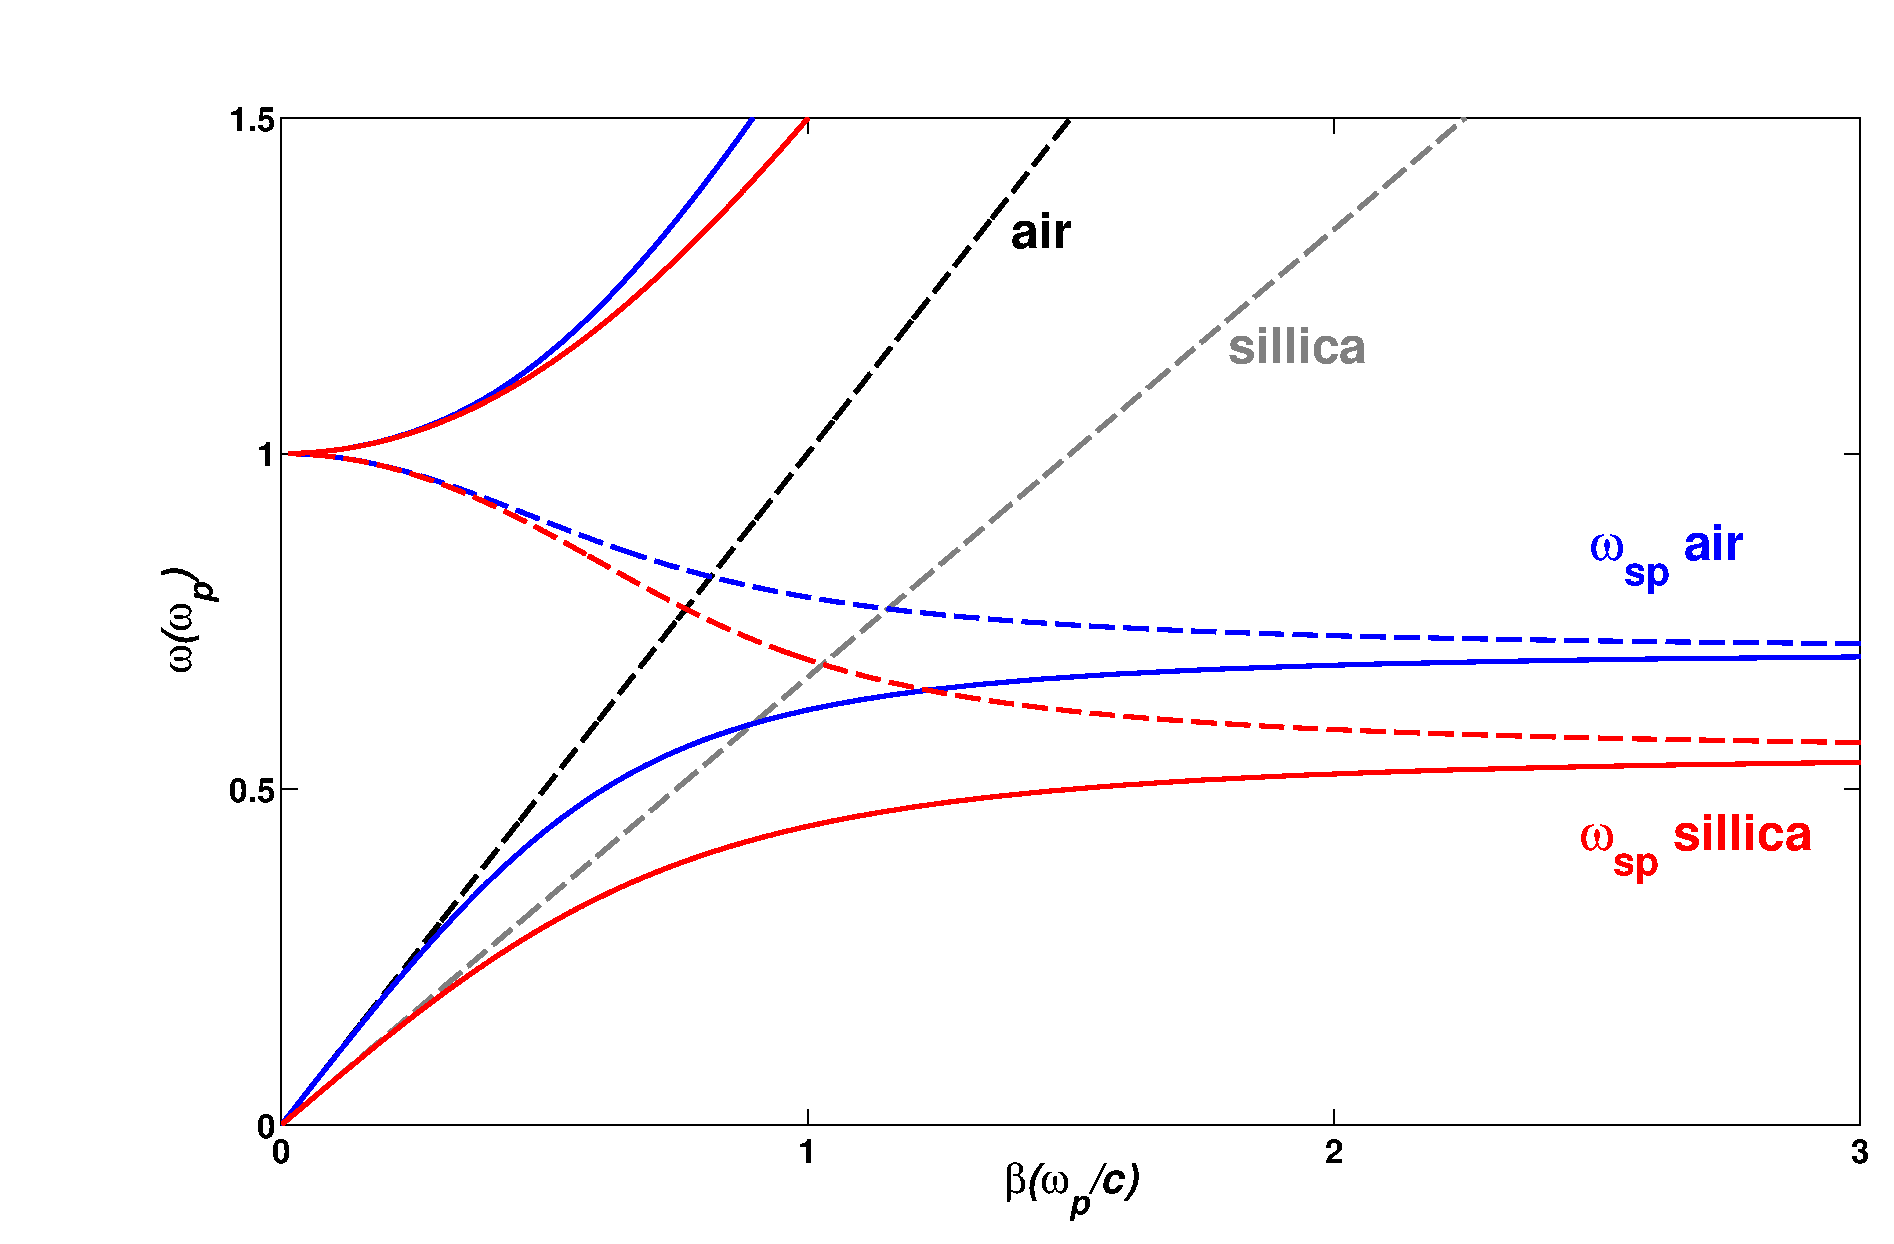
\includegraphics[scale=0.4]{THM/SPPdisp.eps}
\caption{\label{fig:SPPdisp}Dispersion relation of SPPs at the interface between a Drude metal with negligible collision frequency and air (blue curves) and silica (red curves).}
\end{figure}
For small wave vectors SPPs propagation constant $\beta$ is close to $k_0$ at the light line, in the opposite regime of the frequency close to surface plasmon frequency $\omega_p$. It also shows that the SPPs line lying to the right of the respective light lines of air and silica, so that SPPs are directed by light due to phase mismatching. The wave vector mismatch between SPPs and radiation modes needs to be overcome in order to excite or detect SPPs. This can be achieved by multiple methods~\cite{raether1988surface}. In the Otto configuration, light in a prism that is brought in close vicinity to a metal surface can excite SPPs through coupling to the evanescent field. Because light in the prism has a larger wave vector than that in air, it can be phase-matched to the SPPs. In the related Kretschmann-Raether geometry, coupling to SPPs occurs through a metal film that is deposited on a prism. In the grating coupling configuration, metal surface with a shallow grating of grooves or holes with lattice constant $a$. For the simple 1D grating of grooves depicted in Figure~\ref{fig:grating},
\begin{figure}[htb]
\centering
\includegraphics[scale=0.5]{THM/grating.eps}
\caption{\label{fig:grating}Phase-matching of light to SPPs the grating coupling configuration.}
\end{figure}
phase-matching takes place when the condition is fulfilled
\begin{equation}
\beta = k_0 \sin{\theta} \pm \nu g\text{,}
\end{equation}
where $g=\frac{2\pi}{a}$ is the reciprocal vector of the grating, and $\nu=(1,2,3\dots)$.
As with prism coupling, excitation of SPPs is detected as a minimum in the reflected light. The reverse process can also take place, SPPs propagating along a surface modulated with a grating can couple to light and thus radiate. 

%\bibliographystyle{unsrt}
%\bibliography{thesisbib}
%\chapter{Experiment}
\label{c:exp}

\section{Atomic force microscopy}

\begin{figure}[htb]
\centering
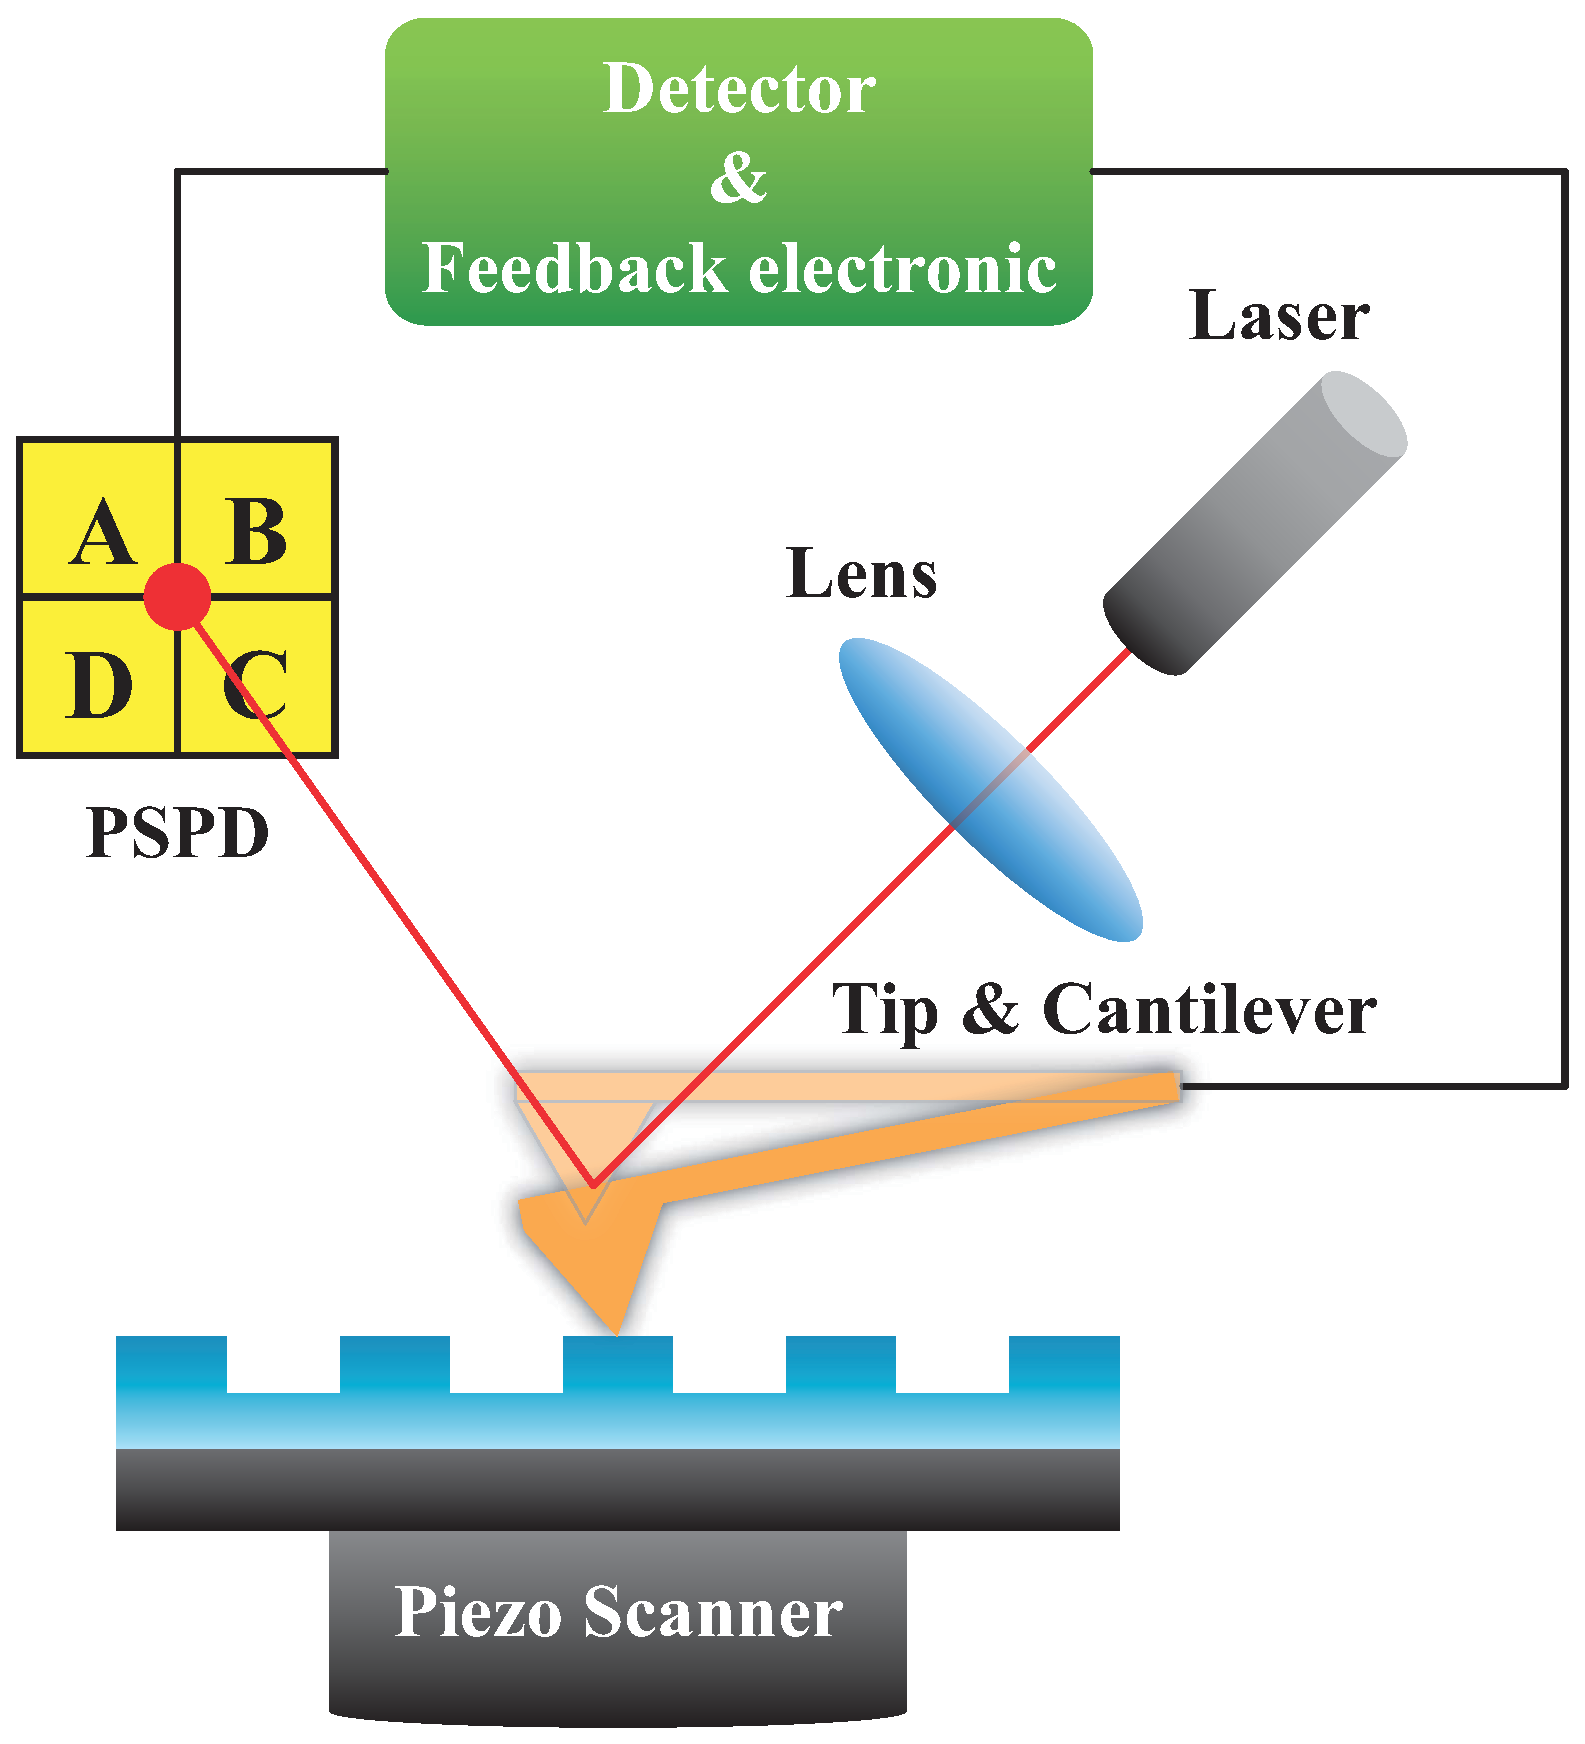
\includegraphics[scale=0.35]{EXP/afm1.eps}
\caption{\label{fig:afm1}Schematic of atomic force microscopy.}
\end{figure}
Atomic force microscope (AFM) is a type of scanning probe microscopes (SPM)~\cite{bennig1988atomic}.  The schematic of AFM is shown in Figure~\ref{fig:afm1}. AFM operates by measuring force between a probe and the specimen surfaces. In general,  the probe is a sharp tip at a cantilever's end. The cantilever can be deflected by atomic forces to sufficiently large amount, then AFM can measure the vertical and lateral deflections of the cantilever by using the optical system. A laser beam is transmitted to cantilever, and the reflected laser beam is detected with a position-sensitive photo detector (PSPD). PSPD is four-sectional that allows measuring not only vertical but lateral bending too(Figure~\ref{fig:afm2}). The output of the PSPD is provided to a computer for processing of the data for providing a topographical image of the surface with atomic resolution, and controlling the height between probe and specimen surfaces by applying voltage on piezoelectric scanner.
\begin{figure}[htb]
\centering
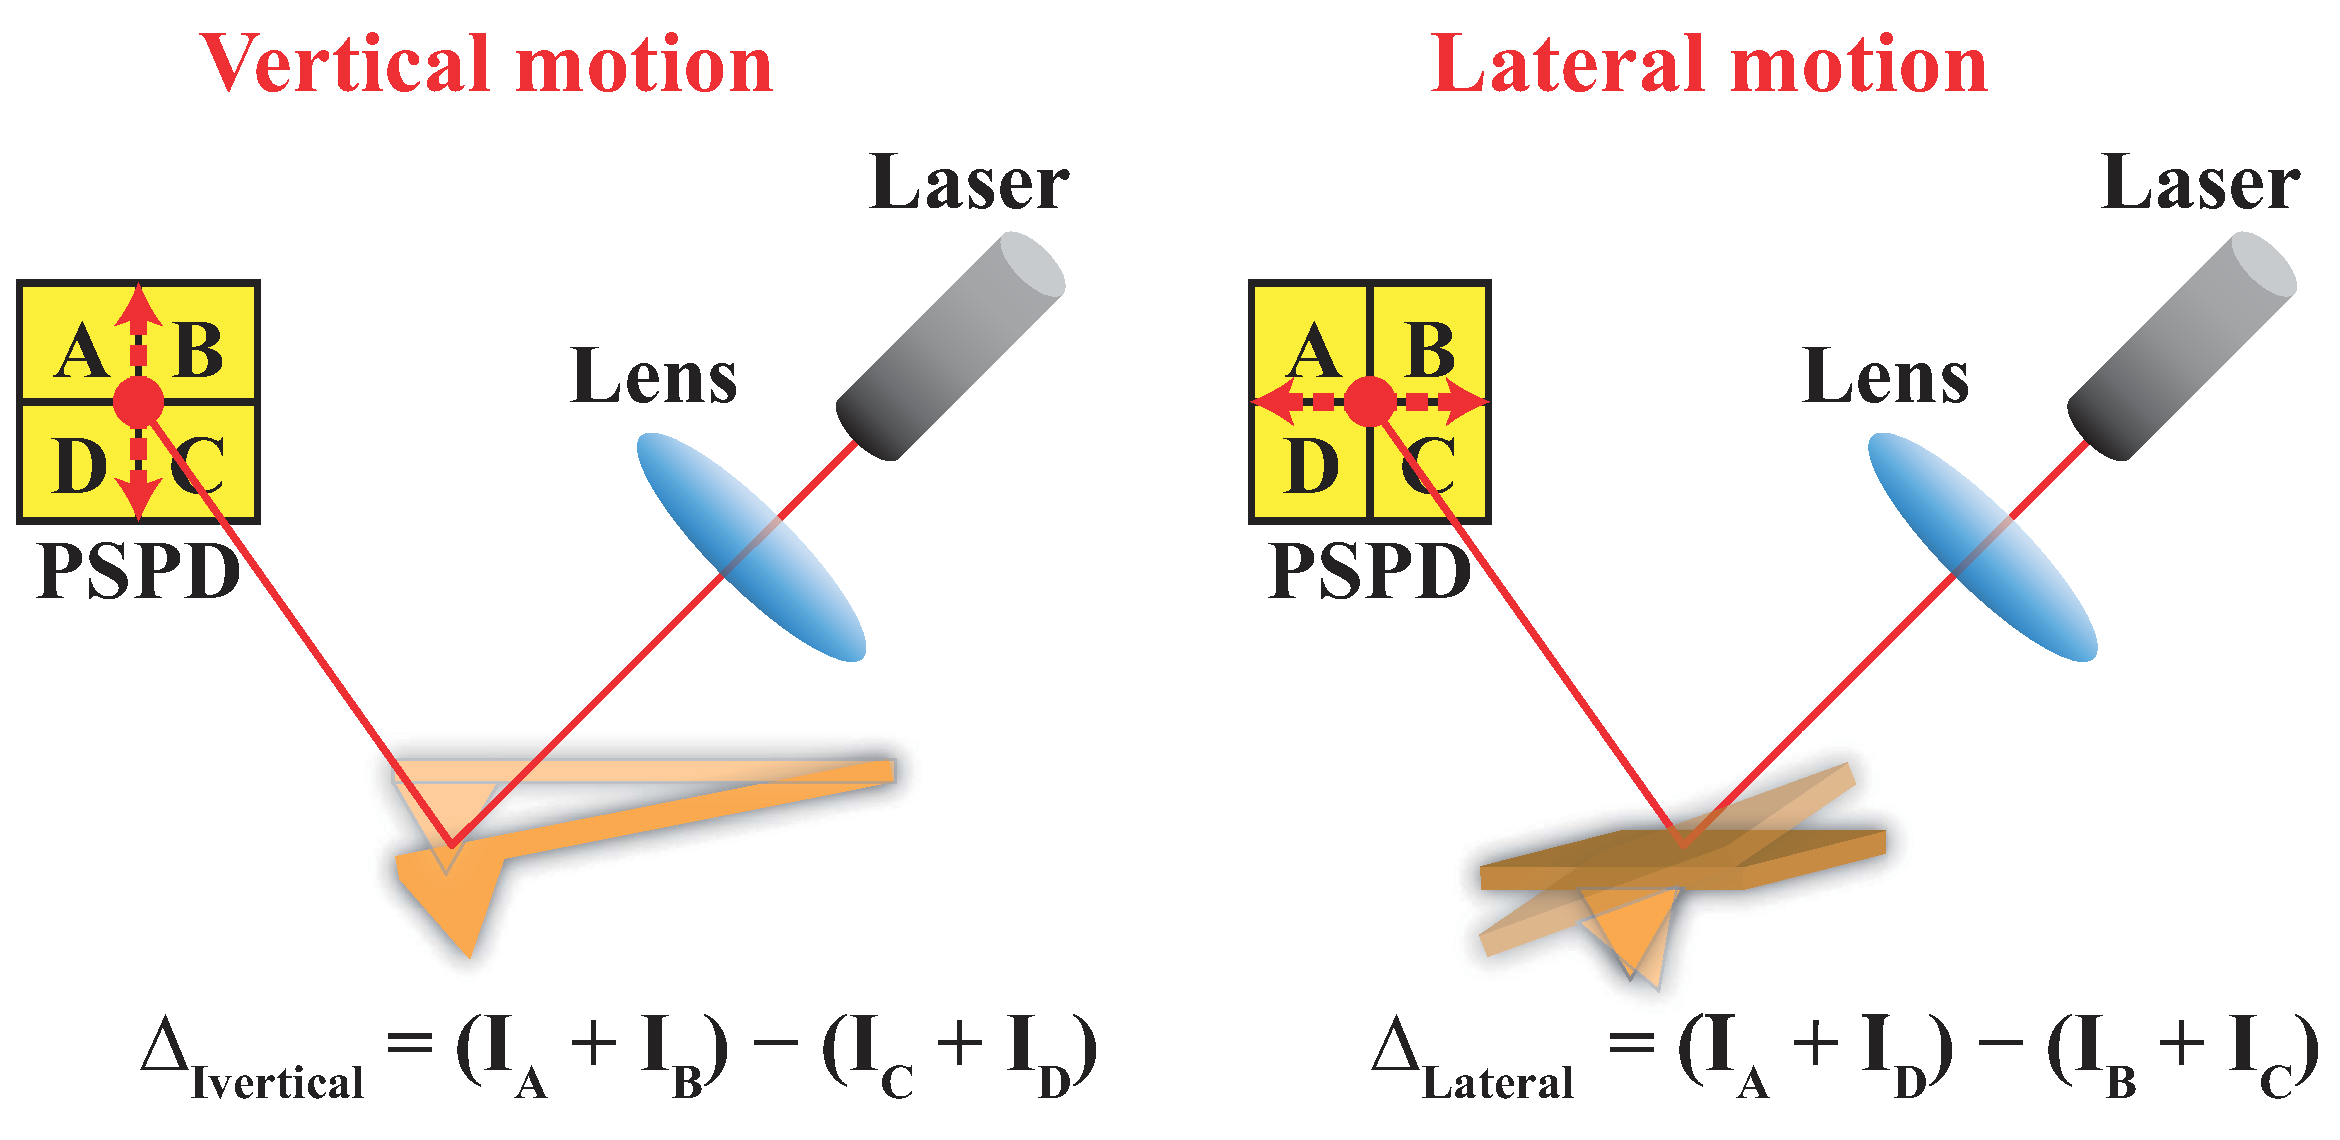
\includegraphics[scale=0.4]{EXP/afm2.eps}
\caption{\label{fig:afm2}Schematic of optical system for cantilever deflections detection.}
\end{figure}

The physical principle of the AFM operation is based on interaction between the probe tip and the specimen surface(Figure~\ref{fig:afm3}). When the cantilever approaches the specimen surface, Van der Waals forces start acting upon it . They are sufficiently far-ranging and are felt at the distance of a few tens of angstroms. Then at the distance of several angstroms repulsive force starts acting. In humid air a water layer is present on the specimen surface. The capillary force arises that holds the tip in contact with the surface and increases the minimum achievable interaction force. Electrostatic interaction between the probe and the sample may appear rather often. This can be both attraction and repulsion. Van der Waals attraction forces, capillary, electrostatic and repulsion forces at the point where the tip touches the sample and forces acting upon the tip from the deformed cantilever compensate each other in equilibrium. Based on the type and degree of this interaction the AFM modes can be broken down into contact and semi-contact(Figure~\ref{fig:afm3} ), which is a transition mode between the contact and non-contact modes.
\begin{figure}[htb]
\centering
\includegraphics[scale=0.6]{EXP/afm3.eps}
\caption{\label{fig:afm3}Sketch of tip-sample forces.}
\end{figure}

\paragraph{Contact mode}

In contact mode of operation the cantilever deflection under scanning reflects repulsive force acting upon the tip. Repulsion force $\mathbf{F}$ acting upon the tip is related to the cantilever deflection value $\mathbf{x}$ under Hooke's law: $\mathbf{F}=-K \cdot  \mathbf{x}$, where $K$ is cantilever spring constant. The spring constant values for different cantilevers usually vary from 0.01 to several $\mathbf{N/m}$.

In our units the vertical cantilever deflection value is measured by means of the optical registration system and converted into electrical signal DFL (difference signal between the upper and lower halves of the PSPD) . In contact mode the DFL signal is used as a parameter characterizing the interaction force between the tip and the surface. There is a linear relationship between the DFL value and the force. In constant force mode of operation the deflection of the cantilever is maintained by the feedback circuitry on the preset value. So vertical displacement of the scanner under scanning reflects topography of sample under investigation.

Contact force microscopy is surface topography measurement in the contact mode.The microscope operation in the mode of maintaining constant interaction force between the tip and the surface sample, and is the base for measuring surface topography as well as for measuring local rigidity, local viscosity and local friction force. Constant force mode has some advantages and disadvantages. Main advantage of constant force mode is possible to measure with high resolution simultaneously with topography and some other characteristics, such as friction forces, spreading resistance etc. Constant force mode has also some disadvantages. Speed of scanning is restricted by the response time of feedback system. When exploring soft samples they can be destroyed by the scratching because the probe scanning tip is in direct contact with the surface. Therefore, under scanning soft unhomogeneous samples the local flexure of sample surface varies. As a result acquired topography of the sample can be proved distorted. Possible existence of substantial capillary forces imposed by a liquid adsorption layer can decrease the resolution.

\paragraph{Semi-contact mode}

The semi-contac mode can be characterized by some advantages in comparison with contact mode. First of all, in this mode the force of pressure of the cantilever onto the surface is less, that allows to work with softer materials such as polymers and bio-organics. The semi contact mode is also more sensitive to the interaction with the surface that gives a possibility to investigate some characteristics of the surface distribution of magnetic and electric domains, elasticity and viscosity of the surface. 

Widely used semi-contact mode has some disadvantage concerned with the usage of the feedback circuit. The scanning speed in semi-contact mode is restricted by the feedback circuit reaction time. This disadvantage can be overcome by the fact that under scanning new value of cantilever oscillation amplitude (and error signal) usually is achieved faster than preset value of the cantilever oscillation amplitude can be reached by the feedback system. Time of the reaching new value of the oscillation amplitude is determined by the oscillation period and Q-quality of the cantilever.
The feedback error signal, emerging when scanning in the semi-contact mode, contains some additional information about the topography. It can be utilized for achieving a more precise recovery of the relief. 

Additionally, similarly to the contact error mode, which can be considered as intermediate between the constant force mode and constant height mode, the feedback gain factor (i.e. the feedback processing speed) can be adjusted for the system to be able to trace subtle changes of the relief and to be too slow to trace the steep changes. Then, when the probe travels over minor irregularities, scanning will be carried out with an almost constant piezo scanner length. As a result, the slow changes of the relief will hardly show up on the images, and the steep changes will appear in high contrast. This may be helpful in finding minor irregularities on large areas against major sloping relief features. It must be noted that height of the minor irregularities must be less than amplitude of cantilever oscillation.

\section{Scanning electron microscopy}

The scanning electron microscope (SEM) is used for the observation of specimen surfaces~\cite{von1938elektronen}. When the specimen is irradiated with a fine electron beam, secondary electrons are emitted from the specimen surface. Topography of the surface can be observed by two-dimensional scanning of the electron probe over the surface and acquisition of an image from the detected secondary electrons. The concept schematic of commercial SEM (JEOL, JSM-6500F) is shown in Figure~\ref{fig:sem1}. The basic unit is composed of an electron optical system, a specimen stage, a secondary-electron detector, an image display unit, and an operation system. The electron optical system consists of an electron gun, a condenser lens and an objective lens to produce an electron probe, a scanning coil to scan the electron probe, and other components. The system inside of the microscope column are kept at vacuum.
\begin{figure}[htb]
\centering
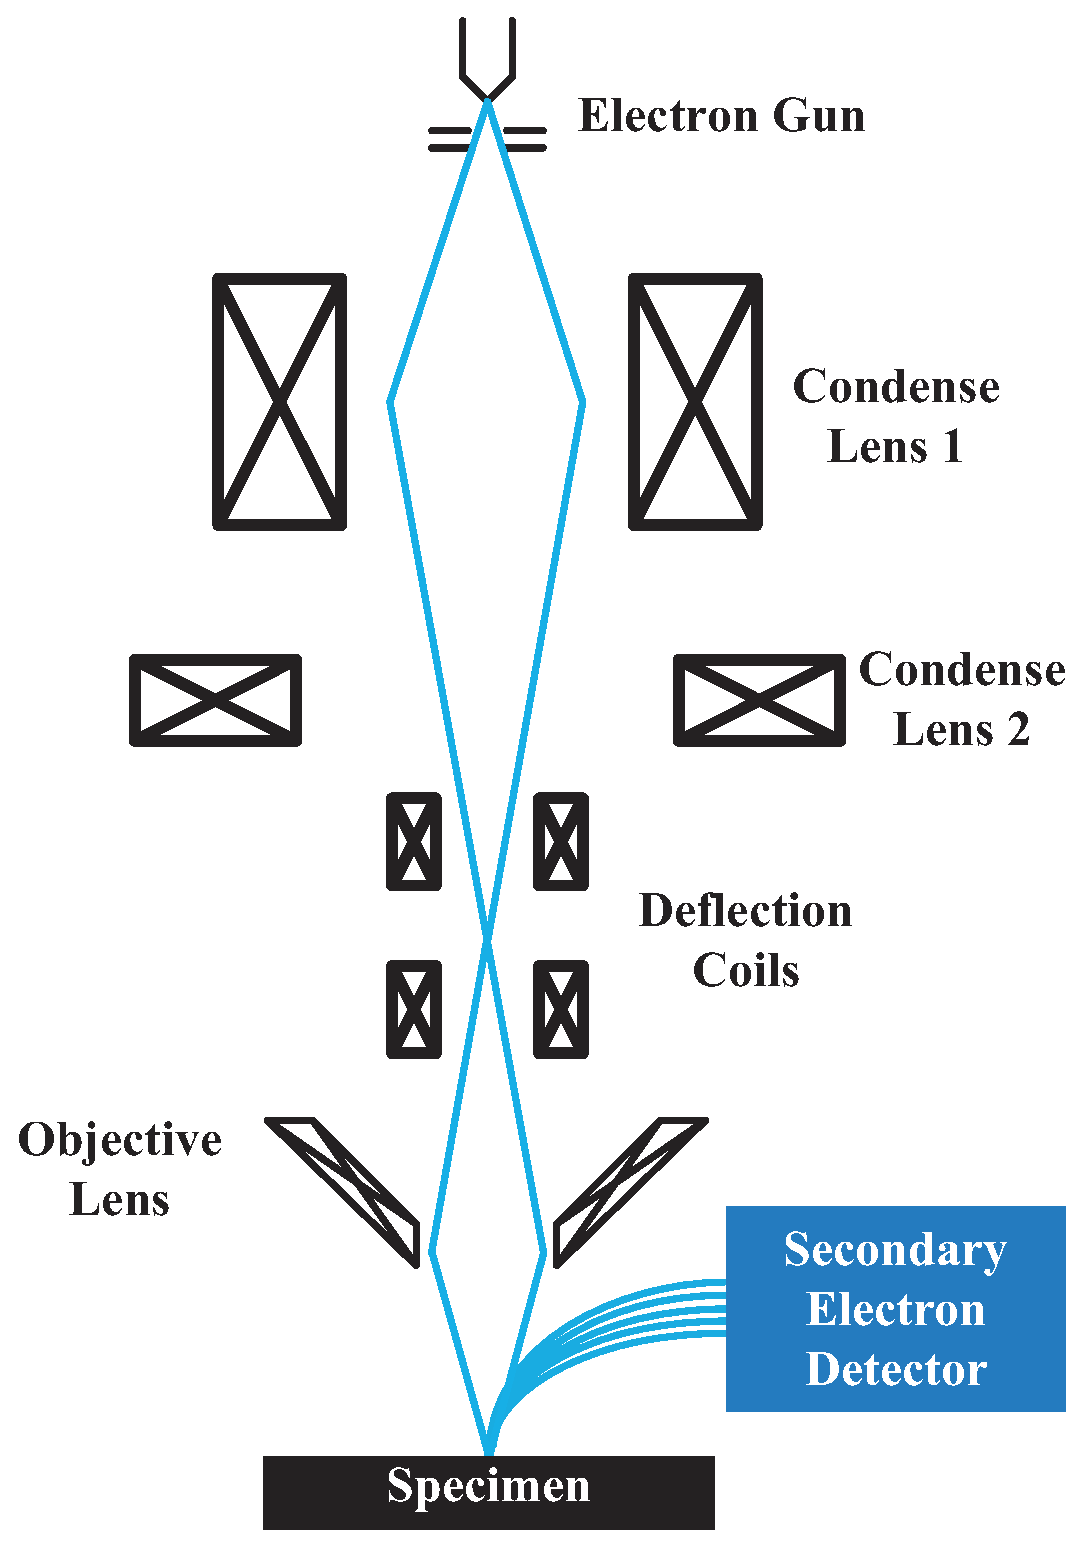
\includegraphics[scale=0.5]{EXP/SEM.eps}
\caption{\label{fig:sem1}Basic construction of a scanning electron microscopy.}
\end{figure}


The JSM-6500F utilizes a Schottky type field-emission (T-FE) gun for the electron source. The T-FE gun can constantly supply the surface of the cathode with zirconium oxide by heating the surface of cathode to 1800 K. For this reason, it can easily obtain stable and high probe current (range from several pA to 100 nA) compared with the traditional thermal emission electron gun and cold field-emission gun.

The magnetic condenser and objective lens system act to control the diameter of the beam as well as to focus the beam on the specimen due to a rotationally-symmetric magnetic field is formed when we pass a direct electric current through a coilwound electric wire in the magnetic lens. A pair of deflector coils, which between the condenser and objective lens, controlled by the scan generator, which are responsible for rastering that focused beam across the specimen surface. The size of the rastering pattern is under magnification control. The beam is rastered from left to right and top to bottom. There is a one-to-one correspondence between the rastering pattern on the specimen and the rastering pattern used to produce the image on the monitor. The resolution we choose to image at will obviously affect the number of pixels per row as well as the number of rows that constitute the scanned area.

The signal is generated from the specimen, and collected by the detector and subsequently processed to generate the image. That processing takes the intensity of the signal coming from a pixel on the specimen and converts it to a grayscale value of the corresponding monitor pixel. The monitor image is a two dimensional rastered pattern of grayscale values.

With the beam focused on the specimen surface, all we need to do to change magnification is to change the size of the rastered area on the specimen. The size of the monitor raster pattern is constant. Magnification will increase if we reduce the size of the area scanned on the specimen.

%\bibliographystyle{unsrt}
%\bibliography{thesisbib}
%\include{main}
%\chapter{Conclusions}
\label{c:conclusions}



\backmatter

%---------- Input your reference here ---------
\bibliographystyle{unsrt}
\addcontentsline{toc}{chapter}{\bibname}
\bibliography{thesisbib}

%----------- Input your appendix here  -----------
%\input{appendixA}

\end{document}
